% Options for packages loaded elsewhere
\PassOptionsToPackage{unicode}{hyperref}
\PassOptionsToPackage{hyphens}{url}
%
\documentclass[
]{book}
\usepackage{amsmath,amssymb}
\usepackage{iftex}
\ifPDFTeX
  \usepackage[T1]{fontenc}
  \usepackage[utf8]{inputenc}
  \usepackage{textcomp} % provide euro and other symbols
\else % if luatex or xetex
  \usepackage{unicode-math} % this also loads fontspec
  \defaultfontfeatures{Scale=MatchLowercase}
  \defaultfontfeatures[\rmfamily]{Ligatures=TeX,Scale=1}
\fi
\usepackage{lmodern}
\ifPDFTeX\else
  % xetex/luatex font selection
\fi
% Use upquote if available, for straight quotes in verbatim environments
\IfFileExists{upquote.sty}{\usepackage{upquote}}{}
\IfFileExists{microtype.sty}{% use microtype if available
  \usepackage[]{microtype}
  \UseMicrotypeSet[protrusion]{basicmath} % disable protrusion for tt fonts
}{}
\makeatletter
\@ifundefined{KOMAClassName}{% if non-KOMA class
  \IfFileExists{parskip.sty}{%
    \usepackage{parskip}
  }{% else
    \setlength{\parindent}{0pt}
    \setlength{\parskip}{6pt plus 2pt minus 1pt}}
}{% if KOMA class
  \KOMAoptions{parskip=half}}
\makeatother
\usepackage{xcolor}
\usepackage{color}
\usepackage{fancyvrb}
\newcommand{\VerbBar}{|}
\newcommand{\VERB}{\Verb[commandchars=\\\{\}]}
\DefineVerbatimEnvironment{Highlighting}{Verbatim}{commandchars=\\\{\}}
% Add ',fontsize=\small' for more characters per line
\usepackage{framed}
\definecolor{shadecolor}{RGB}{248,248,248}
\newenvironment{Shaded}{\begin{snugshade}}{\end{snugshade}}
\newcommand{\AlertTok}[1]{\textcolor[rgb]{0.94,0.16,0.16}{#1}}
\newcommand{\AnnotationTok}[1]{\textcolor[rgb]{0.56,0.35,0.01}{\textbf{\textit{#1}}}}
\newcommand{\AttributeTok}[1]{\textcolor[rgb]{0.13,0.29,0.53}{#1}}
\newcommand{\BaseNTok}[1]{\textcolor[rgb]{0.00,0.00,0.81}{#1}}
\newcommand{\BuiltInTok}[1]{#1}
\newcommand{\CharTok}[1]{\textcolor[rgb]{0.31,0.60,0.02}{#1}}
\newcommand{\CommentTok}[1]{\textcolor[rgb]{0.56,0.35,0.01}{\textit{#1}}}
\newcommand{\CommentVarTok}[1]{\textcolor[rgb]{0.56,0.35,0.01}{\textbf{\textit{#1}}}}
\newcommand{\ConstantTok}[1]{\textcolor[rgb]{0.56,0.35,0.01}{#1}}
\newcommand{\ControlFlowTok}[1]{\textcolor[rgb]{0.13,0.29,0.53}{\textbf{#1}}}
\newcommand{\DataTypeTok}[1]{\textcolor[rgb]{0.13,0.29,0.53}{#1}}
\newcommand{\DecValTok}[1]{\textcolor[rgb]{0.00,0.00,0.81}{#1}}
\newcommand{\DocumentationTok}[1]{\textcolor[rgb]{0.56,0.35,0.01}{\textbf{\textit{#1}}}}
\newcommand{\ErrorTok}[1]{\textcolor[rgb]{0.64,0.00,0.00}{\textbf{#1}}}
\newcommand{\ExtensionTok}[1]{#1}
\newcommand{\FloatTok}[1]{\textcolor[rgb]{0.00,0.00,0.81}{#1}}
\newcommand{\FunctionTok}[1]{\textcolor[rgb]{0.13,0.29,0.53}{\textbf{#1}}}
\newcommand{\ImportTok}[1]{#1}
\newcommand{\InformationTok}[1]{\textcolor[rgb]{0.56,0.35,0.01}{\textbf{\textit{#1}}}}
\newcommand{\KeywordTok}[1]{\textcolor[rgb]{0.13,0.29,0.53}{\textbf{#1}}}
\newcommand{\NormalTok}[1]{#1}
\newcommand{\OperatorTok}[1]{\textcolor[rgb]{0.81,0.36,0.00}{\textbf{#1}}}
\newcommand{\OtherTok}[1]{\textcolor[rgb]{0.56,0.35,0.01}{#1}}
\newcommand{\PreprocessorTok}[1]{\textcolor[rgb]{0.56,0.35,0.01}{\textit{#1}}}
\newcommand{\RegionMarkerTok}[1]{#1}
\newcommand{\SpecialCharTok}[1]{\textcolor[rgb]{0.81,0.36,0.00}{\textbf{#1}}}
\newcommand{\SpecialStringTok}[1]{\textcolor[rgb]{0.31,0.60,0.02}{#1}}
\newcommand{\StringTok}[1]{\textcolor[rgb]{0.31,0.60,0.02}{#1}}
\newcommand{\VariableTok}[1]{\textcolor[rgb]{0.00,0.00,0.00}{#1}}
\newcommand{\VerbatimStringTok}[1]{\textcolor[rgb]{0.31,0.60,0.02}{#1}}
\newcommand{\WarningTok}[1]{\textcolor[rgb]{0.56,0.35,0.01}{\textbf{\textit{#1}}}}
\usepackage{longtable,booktabs,array}
\usepackage{calc} % for calculating minipage widths
% Correct order of tables after \paragraph or \subparagraph
\usepackage{etoolbox}
\makeatletter
\patchcmd\longtable{\par}{\if@noskipsec\mbox{}\fi\par}{}{}
\makeatother
% Allow footnotes in longtable head/foot
\IfFileExists{footnotehyper.sty}{\usepackage{footnotehyper}}{\usepackage{footnote}}
\makesavenoteenv{longtable}
\usepackage{graphicx}
\makeatletter
\newsavebox\pandoc@box
\newcommand*\pandocbounded[1]{% scales image to fit in text height/width
  \sbox\pandoc@box{#1}%
  \Gscale@div\@tempa{\textheight}{\dimexpr\ht\pandoc@box+\dp\pandoc@box\relax}%
  \Gscale@div\@tempb{\linewidth}{\wd\pandoc@box}%
  \ifdim\@tempb\p@<\@tempa\p@\let\@tempa\@tempb\fi% select the smaller of both
  \ifdim\@tempa\p@<\p@\scalebox{\@tempa}{\usebox\pandoc@box}%
  \else\usebox{\pandoc@box}%
  \fi%
}
% Set default figure placement to htbp
\def\fps@figure{htbp}
\makeatother
\usepackage{svg}
\setlength{\emergencystretch}{3em} % prevent overfull lines
\providecommand{\tightlist}{%
  \setlength{\itemsep}{0pt}\setlength{\parskip}{0pt}}
\setcounter{secnumdepth}{5}
% definitions for citeproc citations
\NewDocumentCommand\citeproctext{}{}
\NewDocumentCommand\citeproc{mm}{%
  \begingroup\def\citeproctext{#2}\cite{#1}\endgroup}
\makeatletter
 % allow citations to break across lines
 \let\@cite@ofmt\@firstofone
 % avoid brackets around text for \cite:
 \def\@biblabel#1{}
 \def\@cite#1#2{{#1\if@tempswa , #2\fi}}
\makeatother
\newlength{\cslhangindent}
\setlength{\cslhangindent}{1.5em}
\newlength{\csllabelwidth}
\setlength{\csllabelwidth}{3em}
\newenvironment{CSLReferences}[2] % #1 hanging-indent, #2 entry-spacing
 {\begin{list}{}{%
  \setlength{\itemindent}{0pt}
  \setlength{\leftmargin}{0pt}
  \setlength{\parsep}{0pt}
  % turn on hanging indent if param 1 is 1
  \ifodd #1
   \setlength{\leftmargin}{\cslhangindent}
   \setlength{\itemindent}{-1\cslhangindent}
  \fi
  % set entry spacing
  \setlength{\itemsep}{#2\baselineskip}}}
 {\end{list}}
\usepackage{calc}
\newcommand{\CSLBlock}[1]{\hfill\break\parbox[t]{\linewidth}{\strut\ignorespaces#1\strut}}
\newcommand{\CSLLeftMargin}[1]{\parbox[t]{\csllabelwidth}{\strut#1\strut}}
\newcommand{\CSLRightInline}[1]{\parbox[t]{\linewidth - \csllabelwidth}{\strut#1\strut}}
\newcommand{\CSLIndent}[1]{\hspace{\cslhangindent}#1}
\usepackage{booktabs}
\usepackage{longtable}
\usepackage{array}
\usepackage{multirow}
\usepackage{wrapfig}
\usepackage{float}
\usepackage{colortbl}
\usepackage{pdflscape}
\usepackage{tabu}
\usepackage{threeparttable}
\usepackage{threeparttablex}
\usepackage[normalem]{ulem}
\usepackage{makecell}
\usepackage{xcolor}
\usepackage{bookmark}
\IfFileExists{xurl.sty}{\usepackage{xurl}}{} % add URL line breaks if available
\urlstyle{same}
\hypersetup{
  pdftitle={Mastering Statistical Process Control Charts in Healthcare},
  pdfauthor={Jacob Anhøj \& Mohammed Amin Mohammed},
  hidelinks,
  pdfcreator={LaTeX via pandoc}}

\title{Mastering Statistical Process Control Charts in Healthcare}
\usepackage{etoolbox}
\makeatletter
\providecommand{\subtitle}[1]{% add subtitle to \maketitle
  \apptocmd{\@title}{\par {\large #1 \par}}{}{}
}
\makeatother
\subtitle{A practical, hands-on, step-by-step guide for data scientists using R}
\author{Jacob Anhøj \& Mohammed Amin Mohammed}
\date{2025-06-17}

\begin{document}
\maketitle

{
\setcounter{tocdepth}{1}
\tableofcontents
}
\chapter*{What is Statistical Process Control?}\label{what}
\addcontentsline{toc}{chapter}{What is Statistical Process Control?}

\begin{quote}
This is the online version of \emph{Mastering Statistical Process Control Charts in Healthcare}, a book currently under early development.
\end{quote}

\begin{center}\rule{0.5\linewidth}{0.5pt}\end{center}

The ultimate purpose of collecting and analysing data is to support better decision-making and actions that will lead to improvement. Statistical Process Control (SPC) is a proven methodology for doing just that.

SPC methodology provides a philosophy and framework for continually learning about the behaviour of processes for analytical purposes -- where the aim is to act on the underlying causes of variation to maintain or improve the performance of a process.

SPC was initially developed by Walter A. Shewhart in the 1920s to improve the quality of manufactured products and has since been successfully used in many settings including healthcare.

At is core, SPC methodology involves the plotting of data over time to detect unusual patterns or variations that might indicate a change or problem with a process. This simple graphical device is underpinned by an intuitive theory of variation, the hypothesis-generating testing-cycle of the scientific method, and statistical theory.

To master SPC, it is essential to first understand the underlying theory of variation, which we explore in Part 1 of this book. Next, proficiency in using software to construct SPC charts is key, and this is covered in Part 2. In the later sections, we delve into specialized topics for more advanced SPC practitioners, offering deeper insights and expertise.

\chapter*{Preface}\label{preface}
\addcontentsline{toc}{chapter}{Preface}

This book is about the practical application of \textbf{Statistical Process Control} (SPC) methodology in healthcare.

At its core, SPC is founded on a powerful, intuitive insight: processes are subject to two sources of variation -- \textbf{common cause} and \textbf{special cause}. This distinction enables us to understand, monitor, and improve a wide range of processes. With this insight comes a suite of visual tools -- \textbf{run charts} and \textbf{control charts} -- that help differentiate between common and special cause variation with ease.

However, while SPC tools are conceptually simple to use, applying them correctly can be a challenge. As noted in a systematic review of SPC in healthcare:

\begin{quote}
\ldots{} although SPC charts may be easy to use even for patients, clinicians, or managers without extensive SPC training, they may not be equally simple to \emph{construct correctly}. To apply SPC is, paradoxically, both simple and difficult at the same time.

-- Thor et al. (\citeproc{ref-thor2007}{2007})
\end{quote}

This book seeks to address this paradox by providing a straightforward, practical guide to the correct construction of SPC charts in healthcare using modern software.

\section*{What Sets This Book Apart?}\label{what-sets-this-book-apart}
\addcontentsline{toc}{section}{What Sets This Book Apart?}

This book is a \textbf{step-by-step guide to easily and correctly producing SPC charts}. Since this involves statistics, computing, and visualization, our software of choice is \textbf{R} -- often referred to as the \emph{lingua franca} of statistical computing and visualization.

What makes this book unique is its \textbf{specialized, practical, and modern approach}, specifically tailored for data scientists and practitioners in the healthcare sector. Here's what you can expect:

\begin{enumerate}
\def\labelenumi{\arabic{enumi}.}
\item
  \textbf{Target audience}
  This book is for anyone looking to produce SPC charts using modern tools. While it is specifically geared toward \textbf{data scientists}, we recognize that our readers may include analysts, practitioners, managers, educators, students, researchers, clinicians, or even patients. Regardless of your role, if you work with healthcare data and want to master SPC, then this book is for you.
\item
  \textbf{Why R?}
  We've chosen R as our primary tool because it is popular, free, and open-source. While we are pro-R, we are not anti-other software; readers can adapt the concepts in this book to their preferred tools.
  R has several key advantages:

  \begin{itemize}
  \tightlist
  \item
    \textbf{Transparency and reproducibility}: R's programming capabilities ensure every step of data analysis and SPC chart construction is documented, making your work both readable and reproducible -- something rarely achieved with ``point-and-click'' software.
  \item
    \textbf{Automation}: R allows for automating repetitive tasks such as generating monthly reports, slide decks, and SPC dashboards with customizable, high-quality graphics.
  \end{itemize}
\item
  \textbf{Healthcare-focused}
  Unlike general SPC books, this one focuses on \textbf{healthcare-specific applications}, addressing challenges like patient safety, clinical outcomes, and operational efficiency. It complements the foundational concepts in our companion book, \emph{Statistical Process Control: Elements of Improving Quality and Safety in Healthcare} (\citeproc{ref-mohammed2024}{M. A. Mohammed 2024}).
\item
  \textbf{Practical and hands-on}
  The book takes a hands-on approach, providing real-world examples and case studies to help readers produce and use SPC charts confidently. This practical emphasis bridges the gap between theory and application.
\item
  \textbf{Comprehensive coverage}
  From foundational principles to advanced SPC techniques, this book covers it all. It's designed to cater to both beginners and experienced data scientists, ensuring everyone finds value.
\item
  \textbf{Additional resources}
  Readers will gain access to supplemental materials, including:

  \begin{itemize}
  \tightlist
  \item
    R scripts
  \item
    Datasets
  \item
    A dedicated \href{https://github.com/anhoej/spc4hc}{GitHub repository} for continued learning and collaboration.
  \end{itemize}
\end{enumerate}

\section*{Prerequisites}\label{prerequisites}
\addcontentsline{toc}{section}{Prerequisites}

No prior knowledge of SPC is assumed. However, basic familiarity with R is necessary to follow the steps and algorithms for constructing SPC charts. For those new to R, we recommend excellent (and free) resources such as the \href{https://nhsrcommunity.com/}{NHS-R Community}.

\section*{How to Use This Book}\label{how-to-use-this-book}
\addcontentsline{toc}{section}{How to Use This Book}

\begin{itemize}
\item
  \textbf{New to SPC?}: Start with Chapter \ref{variation} to learn about variation.
\item
  \textbf{Eager to start plotting?}: Jump straight to Chapters \ref{first-chart} and \ref{limits}.
\item
  \textbf{Want to go deeper?}: Advanced chart types and topics are covered in later chapters for both beginners and experts.
\item
  \textbf{Need more resources?}: Visit our \href{https://github.com/anhoej/spc4hc}{GitHub repository} for datasets, code, and updates.
\end{itemize}

We hope this book proves valuable, and we welcome your feedback for ongoing improvement.

\section*{About the Authors}\label{about-the-authors}
\addcontentsline{toc}{section}{About the Authors}

\begin{itemize}
\item
  \textbf{Jacob Anhøj}: Medical doctor with over 30 years of experience and a diploma in Information Technology. With 45+ published papers, two books, and extensive teaching expertise, he is deeply passionate about patient safety and quality improvement in healthcare. Jacob is an experienced R user and the creator of several R packages, including \textbf{qicharts2}, widely used for SPC chart construction and analysis.
  Contact: \href{mailto:jacob@anhoej.net}{\nolinkurl{jacob@anhoej.net}}
\item
  \textbf{Mohammed Amin Mohammed}: Emeritus Professor of Healthcare Quality and Effectiveness at the University of Bradford, Mohammed has over 100 peer-reviewed publications. His landmark paper introducing SPC to healthcare (\citeproc{ref-mohammed2001}{M. A. Mohammed, Cheng, and Marshall 2001}) and his book \emph{Statistical Process Control: Elements of Improving Quality and Safety in Healthcare} (\citeproc{ref-mohammed2024}{M. A. Mohammed 2024}) are seminal works in the field. He is also the founder of the \href{https://nhsrcommunity.com/}{NHS-R Community}, promoting the use of R in healthcare.
  Contact: \href{mailto:profmaminm@gmail.com}{\nolinkurl{profmaminm@gmail.com}}; \href{mailto:m.a.mohammed5@bradford.ac.uk}{\nolinkurl{m.a.mohammed5@bradford.ac.uk}}
\end{itemize}

\chapter*{Synopsis}\label{synopsis}
\addcontentsline{toc}{chapter}{Synopsis}

\section*{Introduction}\label{introduction}
\addcontentsline{toc}{section}{Introduction}

\begin{enumerate}
\def\labelenumi{\arabic{enumi}.}
\tightlist
\item
  What is SPC?
\item
  Preface
\item
  Synopsis
\end{enumerate}

\section*{Part 1: Understanding Variation}\label{part-1-understanding-variation}
\addcontentsline{toc}{section}{Part 1: Understanding Variation}

\begin{enumerate}
\def\labelenumi{\arabic{enumi}.}
\tightlist
\item
  Understanding Variation
\item
  Understanding SPC Charts
\item
  Looking for Signals
\item
  Charts Without Borders -- using runs analysis as stand-alone rules with run charts
\item
  Using SPC in Healthcare
\end{enumerate}

\section*{Part 2: Constructing SPC Charts with R}\label{part-2-constructing-spc-charts-with-r}
\addcontentsline{toc}{section}{Part 2: Constructing SPC Charts with R}

\begin{enumerate}
\def\labelenumi{\arabic{enumi}.}
\tightlist
\item
  Your First SPC Charts with Base R
\item
  Calculating Control Limits
\item
  Highlighting Freaks, Shifts, and Trends
\item
  Core R Functions to Construct SPC Charts
\item
  SPC Charts with ggplot2
\item
  Introducing qicharts2
\end{enumerate}

\begin{center}\rule{0.5\linewidth}{0.5pt}\end{center}

\section*{Part 3: Case Studies and Worked Examples}\label{part-3-case-studies-and-worked-examples}
\addcontentsline{toc}{section}{Part 3: Case Studies and Worked Examples}

\begin{enumerate}
\def\labelenumi{\arabic{enumi}.}
\tightlist
\item
  Case 1
\item
  Case 2
\item
  Case 3
\end{enumerate}

\section*{Part 4: Advanced SPC Techniques}\label{part-4-advanced-spc-techniques}
\addcontentsline{toc}{section}{Part 4: Advanced SPC Techniques}

\begin{enumerate}
\def\labelenumi{\arabic{enumi}.}
\tightlist
\item
  Screened I Chart (eliminating freak moving ranges before calculating limits)
\item
  SPC Charts for Rare Events

  \begin{itemize}
  \tightlist
  \item
    T Charts for Time Between Events
  \item
    G Charts for Opportunities Between Cases
  \item
    Bernoulli CUSUM charts for binary data
  \end{itemize}
\item
  Prime Charts for Count Data with Very Large Subgroups
\item
  I Prime Chart for Measurement Data With Variable Subgroup Sizes
\item
  Funnel Plots for Categorical Subgroups
\item
  Pareto Charts for Ranking Problems
\item
  Dual charting (omit?)
\end{enumerate}

\section*{Part 5: Best Practices, Controversies, and Tips}\label{part-5-best-practices-controversies-and-tips}
\addcontentsline{toc}{section}{Part 5: Best Practices, Controversies, and Tips}

\begin{enumerate}
\def\labelenumi{\arabic{enumi}.}
\tightlist
\item
  Tips for Effective SPC Implementation

  \begin{itemize}
  \tightlist
  \item
    Automating production of SPC charts
  \item
    Engaging stakeholders
  \item
    Continuous monitoring and improvement.
  \item
    Problems and challenges with SPC
  \end{itemize}
\item
  Common Pitfalls to Avoid

  \begin{itemize}
  \tightlist
  \item
    Data issues, misinterpretation of charts
  \item
    Overreacting to common cause variation (over-sensitive runs rules, too tight control limits)
  \item
    Automating recalculation of control limits
  \item
    One-to-one relation between PDSA cycles and dots on the plot
  \item
    The Control Charts vs Run Charts Debate
  \end{itemize}
\item
  A Note on Rational Subgrouping and Sampling
\item
  High Volume Data
\item
  Scaling Up Charts (technical issues, tabular charts, grids)
\item
  When to Transform Data Before Plotting (omit?)
\end{enumerate}

\section*{Part 6: Conclusion and Final Thoughts}\label{part-6-conclusion-and-final-thoughts}
\addcontentsline{toc}{section}{Part 6: Conclusion and Final Thoughts}

\begin{enumerate}
\def\labelenumi{\arabic{enumi}.}
\tightlist
\item
  Summary of Key Points
\item
  Emerging trends in SPC and healthcare analytics
\item
  Encouragement for Continuous Learning and Application
\item
  Final Thoughts
\end{enumerate}

\section*{Appendices}\label{appendices}
\addcontentsline{toc}{section}{Appendices}

\begin{enumerate}
\def\labelenumi{\alph{enumi}.}
\tightlist
\item
  Included Data Sets
\item
  Basic Statistical Concepts
\item
  Diagnostic Properties of SPC Charts (Two Types of Errors When Using SPC)
\item
  A Note on R
\item
  Table of Critical Values for Longest Runs and Number of Crossings
\item
  Resources and Further Readings
\item
  Glossary of Terms
\end{enumerate}

\begin{center}\rule{0.5\linewidth}{0.5pt}\end{center}

\begin{itemize}
\tightlist
\item
  Ideas for chapters / topics

  \begin{itemize}
  \tightlist
  \item
    Improved Runs Analysis Using the Bestbox and Cutbox approaches
  \item
    CUSUM and EWMA Charts
  \item
    Multivariate charts
  \end{itemize}
\end{itemize}

\begin{center}\rule{0.5\linewidth}{0.5pt}\end{center}

\begin{itemize}
\tightlist
\item
  Ideas for papers:

  \begin{itemize}
  \tightlist
  \item
    RAGs to RICHes (two voices)
  \item
    Big data issues -- CUSUM vs 3000 SPC charts
  \item
    Improved I chart
  \item
    The problem with SPC
  \end{itemize}
\end{itemize}

\part*{Part 1: Understanding Variation}\label{part-part-1-understanding-variation}
\addcontentsline{toc}{part}{Part 1: Understanding Variation}

\chapter{Understanding Variation}\label{variation}

Imagine writing the letter a by hand using pen and paper. Figure \ref{fig:variation-fig1} shows eight instances of this letter written by one of the authors. The first seven letters were produced with the dominant (right) hand, while the last one was written with the non-dominant hand.

\begin{figure}
\includegraphics[width=8.53in]{figures/handwritten1} \caption{Hanwritten a's}\label{fig:variation-fig1}
\end{figure}

Consider the seven leftmost a's. Although these a's were produced under identical conditions -- same hand, date, time, place, pen, paper, temperature, lighting, and other factors -- they are not identical. Instead, they exhibit controlled variation. This illustrates that a stable process, where the underlying conditions are the same, produces some degree of variation or ``noise''. This controlled variation is known as common cause variation because it is caused by a stable process.

When examining common cause variation, one might be tempted to rank the letters, identifying some as ``better'' or ``worse'' and attempting to emulate the best while avoiding the worst. However, this approach is misguided. Because all seven letters were produced under the same conditions, no single letter is inherently superior or inferior. From the process perspective, these seven letters are equivalent, and their differences are attributable to common cause variation -- variation intrinsic to the process itself. So how can we improve these a's? To improve the quality of the a's we should focus on modifying the process rather than trying to draw lessons from the differences between individual a's.

To reduce variation and improve the quality of the letter a, we might consider changes such as using a different pen, paper, or training, or switching to a computer. Of these options, it is intuitive that using a computer will yield the most significant improvement. This insight is supported by the theory of constraints, which views a process as a chain of interconnected links. The strength of the entire chain is limited by its weakest link. Improving this weakest link will enhance the overall performance, while changes to other, non-constraint links, offer minimal benefit. In the context of handwriting, the weakest link is the manual use of the hand. The pen, paper, and lighting are not constraints in this process; altering them will not substantially impact the quality of the `a'. Switching to a computer addresses the key constraint, handwriting, resulting in a marked improvement in the quality of the letter.

Now consider the rightmost letter in Figure \ref{fig:variation-fig1}, produced with the non-dominant hand. Its marked difference from the others suggests a special cause. Special cause variation arises from factors external to the usual process and requires investigation. When encountering special cause variation, the response involves detective work to identify the underlying cause.

If the special cause undermines the quality of the process, efforts should focus on eliminating it.
If the special cause enhances the quality of the process, then efforts should focus on trying to understand it and integrate it into the process where possible.

The handwritten letters exemplify the two types of variation:

\begin{itemize}
\item
  Common Cause Variation: Intrinsic to the process, this variation is stable and predictable within a range. Addressing it requires systemic changes to the process as a whole.
\item
  Special Cause Variation: Arising from external factors, this variation is unpredictable and requires investigation. The response depends on whether the variation is beneficial or harmful.
\end{itemize}

In summary then, the handwritten a's demonstrate that a process exhibits two types of variation --- common cause and special cause -- and the action required to address each type of cause is fundamentally different. To address common cause variation, we must take action on a major portion of the process. To address special cause variation, we must first do some detective work to find the cause and then we can decide to eradicate that cause (if it is unfavourable) or keep it (if it is favourable).

The originator of this theory was Walter A. Shewhart, who, in the 1920s, sought to improve industrial product quality. Shewhart recognized that quality involves more than meeting specifications; it requires understanding and managing variation. He distinguished between common cause variation, inherent to a stable process, and special cause variation, which results from specific, external factors (\citeproc{ref-shewhart1931}{Shewhart 1931}).

There are various characteristics and descriptions of common and special cause variation which are highlighted below.

\begin{longtable}[]{@{}
  >{\raggedright\arraybackslash}p{(\linewidth - 2\tabcolsep) * \real{0.5185}}
  >{\raggedright\arraybackslash}p{(\linewidth - 2\tabcolsep) * \real{0.4815}}@{}}
\caption{Characteristics of common versus special cause variation}\tabularnewline
\toprule\noalign{}
\begin{minipage}[b]{\linewidth}\raggedright
Common Cause Variation
\end{minipage} & \begin{minipage}[b]{\linewidth}\raggedright
Special Cause Variation
\end{minipage} \\
\midrule\noalign{}
\endfirsthead
\toprule\noalign{}
\begin{minipage}[b]{\linewidth}\raggedright
Common Cause Variation
\end{minipage} & \begin{minipage}[b]{\linewidth}\raggedright
Special Cause Variation
\end{minipage} \\
\midrule\noalign{}
\endhead
\bottomrule\noalign{}
\endlastfoot
Is caused by a stable process (like
writing a signature) and is intrinsic
to the process. & Is caused by an assignable cause that
it extrinsic to the process. \\
Reflects the voice or behaviour of a
stable process and affects all those
who are part of the process. & Is a distinct signal which differs
from the usual voice or behaviour of
the process and requires further
detective work to identify the
assignable cause. \\
Is neither good or bad, it just is. & Can be favourable or unfavourable and
premediated (as part of an improvement
project) or incidental (not part of an
improvement project) \\
Can be reduced (but not eliminated) by
changing the underlying process.
Such changes may be informed by
special cause variation. & Unfavourable special cause can be
eliminated. Favourable special cause
can be adopted and adapted into a new
process. \\
Is sometimes referred to as random
variation, chance variation, or noise. & Is sometimes referred to as non-random
variation, systematic variation, or
signal. \\
\end{longtable}

\section{SPC and the nature of variation}\label{spc-and-the-nature-of-variation}

Statistical Process Control (SPC) revolves around understanding variation and identifying its causes -- whether common or special -- in order to drive meaningful improvement. Contrary to common misconceptions, SPC is not merely a method for spotting outliers; it's a framework for enhancing processes and outcomes.

\begin{quote}
Statistical Process Control is not about statistics, it is not about `process-hyphen-control', and it is not about conformance to specifications. {[}\ldots{]} It is about the continual improvement of processes and outcomes. And it is, first and foremost, a way of thinking with some tools attached.

-- Wheeler (\citeproc{ref-wheeler2000}{2000}), p.~152
\end{quote}

With this foundation in mind, most of this book focuses on the tools of SPC, particularly the SPC chart. In the next chapter, we delve into the ``anatomy and physiology'' of SPC charts, exploring their structure, function, and practical applications.

\chapter{Understanding SPC Charts}\label{charts-intro}

Now that we've explored the concepts of common and special cause variation through the example of handwritten letters, the next step is understanding how to apply these ideas to healthcare processes. This application involves creating charts that represent the ``voice'' or behaviour of a process (usually) over time. By leveraging statistical theory, these charts help determine whether a process is exhibiting common or special cause variation. Such visualisations are known as SPC charts, control charts, or process behaviour charts.

SPC charts are point-and-line plots of data collected over time. They serve as operational definitions for identifying common and special cause variation. An operational definition is one that is designed to be practical, useful, and ensures consistency in interpretation across different individuals.

\begin{figure}
\centering
\pandocbounded{\includesvg[keepaspectratio]{_main_files/figure-latex/spc-fig0-1.svg}}
\caption{\label{fig:spc-fig0}Control chart of systolic blood pressure}
\end{figure}

Figure \ref{fig:spc-fig0} illustrates a control chart showing daily blood pressure measurements. One data point (\#6), marked with a red dot, stands out from the others. This deviation triggers a signal, indicating that the data point is likely due to a special cause.

Special causes are signalled by unusual patterns in data. By ``unusual'' we mean something that is unlikely to have happened purely by chance, like a freak data point. Common cause variation is simply noise. The absence of signals of special cause variation is evidence that the behaviour of the process is consistent with common cause variation. The presence of signals is consistent with special cause variation.

There are many different types of control charts and the chart to be used is determined mostly by the type of data to be plotted. But regardless of the type of data, (most) SPC charts look the same and are interpreted the same way, by employing a set of statistical tests (or rules) to help identify unusual patterns.

In this chapter, we introduce seven of of the most common types of control charts (The Magnificent Seven) used in healthcare and their practical applications. In the following chapter (\ref{testing}), we delve into the rules and statistical tests for identifying unusual patterns in data. Later, in Part 2 of this book, we provide a detailed guide on performing the calculations necessary to construct and analyse control charts.

\section{Anatomy and physiology of SPC charts}\label{anatomy-and-physiology-of-spc-charts}

Shewhart's groundbreaking innovation was the introduction of control limits, which define the boundaries of common cause variation in data. Data points falling within these limits (without unusual patterns) indicate common cause variation, while those outside indicate special cause variation.

\begin{figure}
\centering
\pandocbounded{\includesvg[keepaspectratio]{_main_files/figure-latex/spc-fig1-1.svg}}
\caption{\label{fig:spc-fig1}Standardised control chart. SD = standard deviation; CL = centre line; LCL = lower control limit; UCL = upper control limit}
\end{figure}

Figure \ref{fig:spc-fig1} demonstrates a standardized Shewhart control chart, created using random numbers from a normal distribution with a mean of 0 and a standard deviation of 1. The x-axis represents time or sequence order, while the y-axis displays the indicator values. Each dot, connected by a line, represents a data point sampled sequentially. The data included in a data point is called a subgroup representing a set of observations (a sample) collected together at a specific point in time and under similar conditions.

The chart features a Centre Line (CL), which represents the mean of the data values, and a Lower Control Limit (LCL) and an Upper Control Limit (UCL), defining the range of common cause variation. Because the control limits are (usually) positioned three standard deviations (sigma) on each side of the centre line they are often referred to as 3-sigma limits.

The data points cluster symmetrically around the centre line, with most near the mean. As the distance from the centre line increases, data points become increasingly sparse. The control limits are positioned to encompass nearly all data points arising from common cause variation. Conversely, points outside the limits are likely to represent special causes.

\section{Why 3-sigma limits?}\label{why-3-sigma-limits}

Shewhart's choice of 3-sigma limits was based on empirical observations from real-world experiments. For data following a normal distribution, like in Figure \ref{fig:spc-fig1}, these limits contain about 99.7\% of all data points, meaning the likelihood of a point falling outside the limits purely by chance is approximately 3 in 1000 (0.3\%). In a control chart with a total of 20 data points the chance of \emph{all} data points being within the control limits is about 95\% (1 - 0.997\textsuperscript{20}).

But before we go down that rabbit hole we note that these theoretical considerations were rejected by Shewhart who found that most real-life data are not normally distributed. Shewhart argued that the choice of 3-sigma limits was made simply because they ``work'' (Shewhart (\citeproc{ref-shewhart1931}{1931}), p.~18), because this practical choice balances sensitivity (detecting special causes) with specificity (avoiding false alarms), regardless of the data type or distribution. More on this will be discussed in Appendix \ref{diagnostics}.

\section{Some common types of control charts: The Magnificent Seven}\label{some-common-types-of-control-charts-the-magnificent-seven}

As described above, the control limits are positioned at three standard deviations (SDs) above and below the centre line. Thus, all types of control charts follow this general formula for control lines:

\[CL \pm 3SD\]

To construct a control chart, the essential components are the process mean and the process standard deviation. However, it is important to use the right standard deviation. Rather than using the overall SD of all data -- which could include variation from special causes and artificially inflate the control limits -- we rely on a pooled average of the within-subgroup SDs. This approach ensures that the calculated control limits reflect only the common cause variation inherent to the process.

The exact method for determining the within-subgroup SD depends on the type of data being analysed. For readers eager to dive into the specifics, the formulas for constructing control limits can be found in Table \ref{tab:limits-tab1} later in the book.

Generally, data come in two flavours: count data and measurement data.

\subsection{Counts}\label{counts}

Counts are positive integers representing the number of events or cases. While the distinction between events and cases may seem subtle, it is crucial for accurate analysis:

\begin{itemize}
\item
  \textbf{Events} are occurrences that happen in time and space, such as patient falls.
\item
  \textbf{Cases} refer to individual units possessing (or lacking) a particular attribute, such as patients who have fallen.
\end{itemize}

When counting events, every occurrence is recorded. For example, if a patient falls multiple times, each fall is counted as a separate event. In contrast, when counting cases, each unit (e.g.~the patient) is counted only once, regardless of how many times the event (e.g.~the fall) occurred for that individual.

Both events and cases can be expressed as ratios, which are counts divided by a relevant denominator, also known as the area of opportunity. However, the way these ratios are constructed depends on whether we are analysing events or cases.

\begin{itemize}
\item
  \textbf{Rates}: Events are often expressed as rates, calculated as the number of events per unit of time. For instance, the rate of falls might be expressed as the number of falls per 1,000 patient-days. The denominator is a continuous variable (e.g., time) and is inherently different from the numerator, which counts discrete events.
\item
  \textbf{Proportions}: Cases are expressed as proportions or percentages, calculated as the number of cases divided by the total number of cases and non-cases. For example, the proportion of patients who fell might represent the percentage of patients who experienced one or more falls. The numerator and denominator represent the same category of count (e.g., patients). The numerator is always a subset of the denominator, meaning it cannot exceed the denominator.
\end{itemize}

The most common chart types for count data are:

\begin{itemize}
\tightlist
\item
  C chart: count of events, e.g.~number of patient falls.
\item
  U chart: event rates, e.g.~number of patient falls per unit of time.
\item
  P chart: case proportions, e.g.~proportion of patients who fell.
\end{itemize}

\subsection{Measurements}\label{measurements}

Measurements refer to data collected on continuous scales, often including decimals. Examples include blood pressure, height, weight, or waiting times.

As an example, consider waiting or ``door-to-needle'' times. These may be plotted as either \textbf{individual} times where each data point represents one patient or as an \textbf{average} time for all patients in a certain period of time, for example an hour, day, week, or month. When producing SPC charts for measurement data, the choice of control chart depends on how the measurement data are grouped.

For individual measurements, we use an I chart (also called an X chart) where each subgroup represents one individual measurement. The I chart is often used in combination with a Moving Range (MR) chart to plot the variability between consecutive individual measurements.

For subgroup averages, we use an X-bar chart where subgroups consist of multiple measurements, such as the average of several patients' waiting times within a given period. the X-bar chart is often used in combination with an S chart to plot the within-subgroup standard deviations, which helps visualize the variability within each subgroup.

\begin{itemize}
\tightlist
\item
  I and MR charts: individual measurement, subgroup size = 1.
\item
  X-bar and S charts: multiple measurements, subgroup size \textgreater{} 1.
\end{itemize}

\section{Summary of common SPC charts}\label{summary-of-common-spc-charts}

A Shewhart control chart is a point-and-line plot of data over time, augmented by three horizontal lines:

\begin{itemize}
\tightlist
\item
  Centre line (CL): Represents the overall mean of the data.
\item
  Lower control limit (LCL) and upper control limit (UCL): Define the boundaries of natural process variation.
\end{itemize}

While there are various types of SPC charts tailored to different types of data, all share a consistent structure and behaviour. When choosing the right chart we must first decide what type of data we have, count data or measurement data:

\begin{itemize}
\tightlist
\item
  \textbf{For count data}:

  \begin{itemize}
  \tightlist
  \item
    C chart: For event counts.
  \item
    U chart: For event rates (events per unit of time or opportunity).
  \item
    P chart: For proportions (cases as a subset of the total).
  \end{itemize}
\item
  \textbf{For measurement data}:

  \begin{itemize}
  \tightlist
  \item
    I chart with MR chart: For individual measurements and moving ranges.
  \item
    X-bar chart with S chart: For subgroup averages and within-subgroup variability.
  \end{itemize}
\end{itemize}

In the next chapter, we will explore the rules and techniques used to detect signals of special causes. We will present a validated set of rules that achieve a high sensitivity to special cause variation while maintaining a reasonable false alarm rate.

\chapter{Looking for Signals on SPC charts -- Beyond the 3-Sigma Rule}\label{testing}

Until now, we have primarily focused on Shewhart's 3-sigma rule, which identifies special cause variation when one or more data points fall outside the control limits.

The 3-sigma rule is effective at detecting large shifts in data. To illustrate:

\textbf{Large shifts (3 SDs)}: Imagine a process with data following a normal distribution that suddenly shifts upward by three standard deviations (SDs). In this case, the old upper control limit (UCL) would effectively become the new centre line (CL). Consequently, about 50\% of subsequent data points would fall above the old UCL, providing a clear signal of the shift.

\textbf{Smaller shifts (1 SD)}: For a smaller shift of one standard deviation, the old UCL would align with the new 2-sigma limit. As a result, about 2.5\% of future data points would exceed this line, signalling the shift but with less frequency.

The 3-sigma rule's sensitivity makes it an invaluable guide for identifying material, easily detectable changes in the behaviour of a process. However, for smaller, subtler shifts, additional rules or techniques are often necessary to ensure reliable detection whilst balancing the number of false alarms (Figure \ref{fig:testing-fig1}).

\begin{figure}
\centering
\pandocbounded{\includesvg[keepaspectratio]{_main_files/figure-latex/testing-fig1-1.svg}}
\caption{\label{fig:testing-fig1}Control chart with progressive shifts in data}
\end{figure}

The performance of the 3-sigma rule has been studied extensively (see, for instance, Montgomery (\citeproc{ref-montgomery2020}{2020}) or Anhøj and Wentzel-Larsen (\citeproc{ref-anhoej2018b}{2018})). To summarize, the 3-sigma rule is most effective when detecting shifts in data of at least 1.5 to 2 standard deviations (SDs). Minor to moderate shifts may go undetected for significant periods. To increase the sensitivity of SPC charts to smaller shifts, a variety of additional rules have been proposed. However, before diving into these rules, it is important to first explore the different patterns in data that often signal the presence of special causes.

\section{Patterns of non-random variation in time series data}\label{patterns-of-non-random-variation-in-time-series-data}

In the iconic Western Electric Handbook (\citeproc{ref-we1956}{Western~Electric~Company 1956}) a variety of control chart patterns are described to assist engineers in interpreting control charts based on the notion that certain patterns often reflect specific causes. In our experience, the most common special cause patterns found in healthcare data are freaks, shifts, and trends.

\subsection{Freaks}\label{freaks}

A freak is a data point or a small number of data points that are distinctly different from the rest, as shown in Figure \ref{fig:testing-fig2}. By definition, freaks are transient -- they appear suddenly and then disappear.

\begin{figure}
\centering
\pandocbounded{\includesvg[keepaspectratio]{_main_files/figure-latex/testing-fig2-1.svg}}
\caption{\label{fig:testing-fig2}Control chart with a large (2 SD) transient shift in data}
\end{figure}

Freaks are often caused by data or sampling errors, but they can also result from temporary external factors influencing the process, such as shifts in patient case mix during a holiday season. In some cases, a freak may simply be a false alarm.

\subsection{Shifts}\label{shifts}

Shifts are caused by sudden and sustained changes in process behaviour as in Figure \ref{fig:testing-fig3}.

\begin{figure}
\centering
\pandocbounded{\includesvg[keepaspectratio]{_main_files/figure-latex/testing-fig3-1.svg}}
\caption{\label{fig:testing-fig3}Control chart with a minor (1 SD) sustained shift in data introduced at data point \#16}
\end{figure}

In fact, in healthcare improvement we strive to induce shifts in the desired direction by improving the structures and procedures that are behind data.

\subsection{Trends}\label{trends}

A trend is a gradual change in the process centre, as shown in Figure \ref{fig:testing-fig4}.

\begin{figure}
\centering
\pandocbounded{\includesvg[keepaspectratio]{_main_files/figure-latex/testing-fig4-1.svg}}
\caption{\label{fig:testing-fig4}Control chart with a trend in data}
\end{figure}

While some texts define a trend more specifically as a series of data points moving consistently up or down, in this book we use the term in a broader sense to refer to any gradual shift in one direction.

Trends occur when external forces are consistently influencing the data in one direction, particularly when this influence is continuous and cumulative. Trends are commonly observed when improvements are implemented incrementally, such as in large organizations. In such cases, sequential shifts in data at the department level may accumulate into a broader trend at the organizational level.

\subsection{Other unusual patterns}\label{other-unusual-patterns}

There are numerous other types of ``unusual'' or mixed patterns that may appear in data. However, based on our experience in healthcare, process improvement or deterioration is most commonly associated with freaks, shifts, or trends. Learning to recognize these patterns is essential for uncovering the underlying causes of change.

That being said, depending on the context and the purpose of using SPC, it may be valuable to look for other types of patterns in the data. This is particularly true for cyclic or seasonal data, where specific patterns repeat based on time of day, week, month, or year (\citeproc{ref-jeppegaard2023}{Jeppegaard et al. 2023}). For example, excess mortality linked to weekend admissions might not present itself as a freak, shift, or trend, but it is still an important pattern to recognize in order to address the issue effectively.

\section{SPC rules}\label{spc-rules}

If patterns of special cause variation were always as clear as in the figures \ref{fig:testing-fig2}, \ref{fig:testing-fig3}, and \ref{fig:testing-fig4} there would be no need for SPC. However, in practice, special causes often manifest in more subtle ways and so we use additional statistical tests or SPC rules that are designed to signal the presence, or rather the likelihood, of special cause variation.

Many additional rules have been developed to identify minor shifts, trends, and other specific patterns in data. While it may seem tempting to apply all known rules to the data, it's important to remember that the more tests we apply, the more signals we generate and this increases the risk of false alarms where common cause variation is mistakenly identified as special cause variation.

Therefore, it is crucial to strike a balance: we must select as few rules as necessary to minimize false alarms while ensuring the detection of true special cause signals. This topic will be discussed in greater detail in the chapter on \hyperref[diagnostics]{Diagnostic Errors} later in this book.

For this book, we will concentrate on two sets of rules that have been thoroughly studied and validated for their effectiveness.

\subsection{Tests based on sigma limits}\label{tests-based-on-sigma-limits}

The best known tests for special cause variation are probably the Western Electric Rules (WE) described in the Statistical Quality Control Handbook (\citeproc{ref-we1956}{Western~Electric~Company 1956}). The WE rules consist of four simple tests that can be applied to control charts by visual inspection and are based on the identification of unusual patterns in the distribution of data points relative to the centre lines and the control limits.

\begin{enumerate}
\def\labelenumi{\arabic{enumi}.}
\item
  One or more points outside of the 3-sigma limits (Shewhart's original 3-sigma rule).
\item
  Two out of three successive points beyond a 2-sigma limit (two thirds of the distance between the centre line and the control line).
\item
  Four out of five successive points beyond a 1-sigma limit.
\item
  A run of eight successive points on one side of the centre line.
\end{enumerate}

We leave it to the reader to apply WE rules \#2-\#4 to figures \ref{fig:testing-fig3} and \ref{fig:testing-fig4}.

The WE rules have proven their worth during most of a century. One thing to notice though is that the WE rules are most effective with control charts that have between 20 and 30 data points. With fewer data points, they lose sensitivity (more false negatives), and with more data points they lose specificity (more false positives).

WE rule \#4 is independent of the sigma limits. It is based on assumptions regarding the length of runs on either side of the centre line. A run is defined as one or more successive data points on the same side of the centre line. Rules based on runs analysis are further discussed below.

\subsection{Runs analysis -- tests based on the distribution of data points around the centre line}\label{runs-analysis-tests-based-on-the-distribution-of-data-points-around-the-centre-line}

If we assume that the centre line divides the data into two halves, the probability of any data point falling above or below the centre is fifty-fifty. Similarly, the probability that two neighbouring points fall on the same or opposite side of the centre line is also fifty-fifty.

By dichotomizing the data into runs of points either above or below a certain value -- such as the centre line -- we enter the realm of runs analysis. The fundamental idea behind runs analysis is that the length and number of runs in a random process are governed by natural laws, making them predictable within certain limits.

In essence, when a process shifts or trends, runs tend to become longer and fewer. Therefore, we can design runs tests to detect unusually long or unusually few runs. The key question is: what constitutes ``unusually'' long or ``unusually'' few runs?

To illustrate, imagine flipping a coin ten times. Would you be surprised to get three or four heads in a row? Probably not. But what if you got ten heads in a row? That would definitely be surprising. Now, imagine tossing the coin 100 times. Would a sequence of ten heads be surprising then? Probably not, because as the number of trials increases, the likelihood of observing a run of ten heads also increases.

This intuitive understanding highlights that what constitutes an ``unusually'' long run depends on the total number of observations or subgroups. The more subgroups we have in our SPC chart, the longer the longest runs are likely to be. From practical experiments, some theoretical considerations (\citeproc{ref-anhoej2014}{Anhøj and Olesen 2014}; \citeproc{ref-anhoej2015}{Anhøj 2015}; \citeproc{ref-anhoej2018b}{Anhøj and Wentzel-Larsen 2018}), and years of experience we suggest these two runs tests:

\begin{itemize}
\item
  \textbf{Unusually long runs}: A run is one or more consecutive data points on the same side of the centre line. Data points that fall directly on the centre line neither break nor contribute to the run. The upper 95\% prediction limit for longest run in a random process is approximately \(log_2(n)+3\) (rounded to the nearest integer), where \(n\) is the number of useful data points (data points not on the centre line). For example, in a run chart with 24 useful data points a run of \emph{more} than \texttt{round(log2(24)\ +\ 3)} = 8 would suggest a shift in the process (\citeproc{ref-schilling2012}{Schilling 2012}).
\item
  \textbf{Unusually few crossings}: Rather than counting the number of runs, we count the number of crossings, which by definition is one less than the number of runs. A crossing is when two consecutive data points are on opposite sides of the centre line. In a random process, the number of crossings follows a binomial distribution. The lower 5\% prediction limit for number of crossings is found using the cumulative probability distribution, \texttt{qbinom(p\ =\ 0.05,\ size\ =\ n\ -\ 1,\ prob\ =\ 0.5)}. Thus, in a run chart with 24 useful data points, \emph{fewer} than \texttt{qbinom(0.05,\ 24\ -\ 1,\ 0.5)} = 8 crossings would suggest that the process is shifting (\citeproc{ref-chen2010}{Chen 2010}).
\end{itemize}

The two runs rules are two sides of the same coin -- when runs get longer, crossings get fewer and vice versa -- and either of them may signal special cause variation.

Figure \ref{fig:testing-fig3} has 24 data points, the longest run consists of 12 data points (\#13 - \#24), and the line crosses the centre line 9 times. Since the longest run is longer than expected, we may conclude that there is reason to believe that the process is shifting.

In Figure \ref{fig:testing-fig4} there are two long runs with 9 data points and only 5 crossings also suggesting that data are shifting.

It is important to note that the tests themselves do not identify the specific types of patterns in the data, nor do they reveal the underlying causes of shifts or trends. The responsibility for interpreting the results lies with the data analyst and the individuals involved in the process. This is the topic of the next chapter (\ref{using}).

Critical values for longest runs and number of crossings for 10-100 data points are tabulated in Appendix \ref{runs-limits}.

Apart from being comparable in sensitivity and specificity to WE rules \#2-\#4 with 20-30 data points (\citeproc{ref-anhoej2018b}{Anhøj and Wentzel-Larsen 2018}), these runs rules have some advantages:

\begin{itemize}
\item
  They do not depend on sigma limits and thus are useful as stand-alone rules with run charts (more on run charts in the next section).
\item
  They adapt dynamically to the number of available data points, and can be applied to charts with as few as 10 and up to indefinitely many data points without losing sensitivity or specificity.
\end{itemize}

In practice these runs rules may be used as alternatives to WE rules \#2-\#4 to help identify shifts and trends alongside the WE rule \#1 for freaks.

\section{SPC charts without borders -- using run charts}\label{spc-charts-without-borders-using-run-charts}

As discussed in the previous section, some rules rely solely on a single line representing the centre of the data. We assumed that the centre line divides the data into two equal halves. While the process average typically serves as a good representation of this centre, this assumption may not hold if the data are skewed. However, if we use the median instead of the mean, the assumption always holds true, because the median is by definition the middle value.

So, what happens if we remove the sigma lines and use the median as the centre line? We get a run chart, which is one of the most valuable tools in quality improvement and control.

\begin{figure}
\centering
\pandocbounded{\includesvg[keepaspectratio]{_main_files/figure-latex/testing-fig5-1.svg}}
\caption{\label{fig:testing-fig5}Run chart}
\end{figure}

Figure \ref{fig:testing-fig5} is a run chart of the data from Figure \ref{fig:spc-fig1}. We notice that the centre line is a little different from the control chart because we have used the empirical median rather than the theoretical mean. Consequently, data are now evenly distributed around the centre line with 12 data points on each side. The longest run have 3 data points (\#13-\#15 and \#22-\#24), and the data line crosses the centre line 13 times. Since there are no unusually long runs and not unusually few crossing we conclude that this process shows no signs of persistent shifts in data.

Figure \ref{fig:testing-fig6} is a run chart with data from Figure \ref{fig:testing-fig4} containing a trend. The runs analysis confirms our ``analysis-by-eye'' by finding two unusually long runs with 9 data points and unusually few crossings (4).

\begin{figure}
\centering
\pandocbounded{\includesvg[keepaspectratio]{_main_files/figure-latex/testing-fig6-1.svg}}
\caption{\label{fig:testing-fig6}Run chart with a trend}
\end{figure}

Run charts are a lot easier to construct than are control charts. They do not make assumptions about the distribution of data. And they have better sensitivity to minor and moderate \emph{persistent} shifts and trends than control charts based on only the 3-sigma rule.

So why do we bother making control charts at all? In fact, we can only think of two reasons: 1) control charts quickly pick up large, possibly transient, shifts (for example freaks) that may go unnoticed by run charts, and 2) the control limits reflect the common cause variability of the process and hence define its \emph{capability}, that is the process' ability to meet specifications.

Fortunately, we do not need to choose between run and control charts. In fact, they are good companions for use at different stages of quality improvement and control.

\section{A practical approach to SPC analysis}\label{a-practical-approach-to-spc-analysis}

Before we move on, let's take a moment to clarify the purpose of SPC charts. As we will explore in detail in the next chapter (see \ref{using}), SPC charts support two distinct purposes: process improvement and process monitoring.

When we are focused on \textbf{process improvement}, our goal is to create sustained shifts in the desired direction. Shifts are expected in this context, as improvements often happen gradually. Since we aim for lasting changes, runs analysis is our primary tool to detect these shifts.

In \textbf{process monitoring}, the objective is to maintain process stability, with no expected shifts in the data. Here, our focus is on detecting any signs of process deterioration as quickly as possible. For this, the 3-sigma rule is effective. To improve sensitivity to minor or moderate shifts, we may combine the 3-sigma rule with \emph{either} the rest of the Western Electric (WE) rules \emph{or} the two runs rules. However, we must be mindful that adding more tests increases the risk of false alarms.

Regardless of the task, we recommend starting any SPC analysis with an ``assumption-free'' run chart, using the median as the centre line. If runs analysis indicates non-random variation, calculating sigma limits becomes meaningless, as these values are irrelevant when shifts are already evident. In such cases, the focus should shift to identifying special causes, rather than calculating control limits.

If the goal is process improvement, we continue with the run chart until we observe significant and sustained improvement, leading to a new and better process. Once this new process stabilizes and appears set to continue, we may transition to monitoring mode by adding control limits and using the mean as the centre line.

Process monitoring is appropriate when the process is stable (common cause variation only) and the outcome is satisfactory. If either condition is not met, we should return to improvement mode.

\section{SPC rules in summary}\label{spc-rules-in-summary}

SPC rules are statistical tests designed to detect special cause variation in time series data. Given the variety of patterns that can indicate special causes, many rules have been developed. However, applying too many rules increases the risk of false alarms. Therefore, it is important to choose a small set of rules that strike a balance: maximizing the ability to detect true alarms (special causes) while minimizing false alarms.

We recommend starting any SPC analysis with a median-based run chart and using the two runs rules to test for unusually long runs or an unusually small number of crossings. If, and only if, the runs analysis indicates random variation (no special cause), and the process outcome is stable and satisfactory, we may proceed to use the mean as the centre line and add control limits to help identify large shifts and freak data points more easily.

\chapter{Using SPC in healthcare}\label{using}

As briefly discussed in the previous chapter, in healthcare, we use SPC methodology in two main ways:

\begin{itemize}
\tightlist
\item
  \textbf{Monitoring} the behaviour or performance of an existing process (e.g.~complications following surgery), or
\item
  \textbf{Improving} an existing process (e.g.~redesigning the pathway for patients with fractured hips).
\end{itemize}

\section{Using SPC to monitor a process}\label{using-spc-to-monitor-a-process}

In the monitoring mode, the primary aim is to determine if a process is deteriorating which is usually indicated by signals of special cause variation where detective work is needed to find the cause and then eliminate it. Such detective work can be undertaken by using the Pyramid Model of Investigation described below.

The key aim of using statistical process control charts to monitor healthcare processes is to ensure that quality and safety of care are adequate and not deteriorating. So when a signal of special cause variation is seen on a control chart monitoring a given outcome, investigation is necessary. However, the chosen method must recognise that the link between recorded outcomes and quality of care \emph{is complex, ambiguous and subject to multiple explanations} (\citeproc{ref-lilford2004}{Lilford et al. 2004}). Failure to do so may inadvertently contribute to premature conclusions and a blame culture that undermines the engagement of clinical staff and the credibility of statistical process control. As Rogers note:

\begin{quote}
If monitoring schemes are to be accepted by those whose outcomes are being assessed, an atmosphere of constructive evaluation, not `blaming' or `naming and shaming', is essential as apparent poor performance could arise for a number of reasons that should be explored systematically.

-- Rogers et al. (\citeproc{ref-rogers2004}{2004})
\end{quote}

To address this need, M. A. Mohammed et al. (\citeproc{ref-mohammed2004}{2004}) proposed the \textbf{Pyramid Model} for Investigation of Special Cause Variation in healthcare -- a systematic approach of hypothesis generation and testing based on five a priori candidate explanations for special cause variation: data, patient casemix, structure/resources, process of care, and carer(s) (Figure \ref{fig:responding-fig1}).

\begin{figure}
\centering
\pandocbounded{\includesvg[keepaspectratio]{figures/pyramid_model.svg}}
\caption{\label{fig:responding-fig1}Pyramid Model for Investigation}
\end{figure}

These broad categories of candidate explanations are arranged from most likely (data) to least likely (carers), so offering a road map for the investigation that begins at the base of the pyramid and stops at the level that provides a credible, evidence-based explanation for the special cause. The first two layers of the model (data and casemix factors) provide a check on the validity of the data and casemix-adjusted analyses, whereas the remaining upper layers focus more on quality of care related issues.

A proper investigation requires a team of people with expertise in each of the layers. Such a team is also likely to include those staff whose outcomes or data are being investigated, so that their insights and expertise can inform the investigation while also ensuring their buy-in to the investigation process. Basic steps for using the model are shown below.

\begin{enumerate}
\def\labelenumi{\arabic{enumi}.}
\item
  Form a \textbf{multidisciplinary team} that has expertise in each layer of the pyramid, with a decision-making process that allows them to judge the extent to which a credible cause or explanation has been found, based on hypothesis generation and testing.
\item
  Guided by what type(s) of pattern(s) exist in data (freaks, shifts, trends, mixed, or cyclic patterns) candidate \textbf{hypotheses} are generated and tested starting from the lowest level of the Pyramid Model and proceeding to upper levels only if the preceding levels provide no adequate explanation for the special cause.
\item
  A credible cause requires \textbf{quantitative and qualitative evidence}, which is used by the team to test hypotheses and reach closure. If no credible explanation can be found, then the only plausible conclusion is that the signal itself was a false signal.
\end{enumerate}

The types of questions that can be asked when undertaking the detective work are highlighted below.

\begin{itemize}
\tightlist
\item
  \textbf{Data}: Data quality issues, e.g.~coding accuracy, reliability of charts, definitions, and completeness.

  \begin{itemize}
  \tightlist
  \item
    Are the data coded correctly?
  \item
    Has there been a change in data coding practices (e.g.~are there less experienced coders)?
  \item
    Is clinical documentation clear, complete, and consistent?
  \end{itemize}
\item
  \textbf{Casemix}: Although differences in casemix are accounted for in the calculation, it is possible that some residual confounding may remain.

  \begin{itemize}
  \tightlist
  \item
    Are factors peculiar to this hospital not taken into account in the risk adjustment?
  \item
    Has the pattern of referrals to this hospital changed in a way not considered in risk adjustment?
  \end{itemize}
\item
  \textbf{Structure or resource}: Availability of beds, staff, and medical equipment; institutional processes.

  \begin{itemize}
  \tightlist
  \item
    Has there been a change in the distribution of patients in the hospital, with more patients in this speciality spread throughout the hospital rather than concentrated in a particular unit?
  \item
    Has the physical environment or organisational structures changed?
  \end{itemize}
\item
  \textbf{Process of care}: Medical treatments, clinical pathways, patient admission and discharge policies.

  \begin{itemize}
  \tightlist
  \item
    Has there been a change in the care being provided?
  \item
    Have new treatment guidelines been introduced?
  \end{itemize}
\item
  \textbf{Professional staff/carers}: Practice and treatment methods etc.

  \begin{itemize}
  \tightlist
  \item
    Has there been a change in staffing for treatment of patients?
  \item
    Has a key staff member gained additional training and introduced a new method that has led to improved outcomes?
  \end{itemize}
\end{itemize}

\section{Using SPC to improve a process}\label{using-spc-to-improve-a-process}

SPC is also used to support efforts to improve a process. In healthcare, this usually involves making small scale changes and measuring their impact on an SPC chart. In the improving mode, the primary aim is to determine if changes made to a process have been successful (or not). For example, in the handwriting process considered earlier, do we get better a's after switching to a computer? This is determined by looking to see the impact of the change in the form of signals of special cause variation on an SPC chart (provided we have a creditable measure of ``letter quality'').

The degree of alignment between changes to the process and subsequent signals of special cause variation provide a story which qualitatively and quantitatively describes the impact of changes.

Common cause variation can only be addressed by changing a major portion of the process. What do we mean by a major portion? \textbf{The Theory of Constraints} (\citeproc{ref-goldratt2022}{Goldratt and Cox 2022}) offers the analogy of a chain to demonstrate that the strength of the chain is determined by the weakest link. If we increase the strength of the weakest link the whole chain is strengthened. If we increase the strength of other links but not the weakest link, then the chain does not get stronger. The weakest link is the constraint on the performance of the system, and it is argued that in real systems there are usually only a few, perhaps one or two, constraining factors, all other factors are non-constraints.

\textbf{The Model for Improvement}, proposed by Langley et al. (\citeproc{ref-langley2009}{2009}), is a widely used framework in healthcare to guide improvement efforts. It consists of three fundamental questions and the Plan-Do-Study-Act (PDSA) cycle.

\begin{enumerate}
\def\labelenumi{\arabic{enumi}.}
\item
  \textbf{What are we trying to accomplish?}
  This question defines the aim of the improvement effort, which should be specific, measurable, and time-bound along with a rationale for why this is important.
\item
  \textbf{How will we know that a change is an improvement?}
  This question focuses on measurement. The team identifies key performance indicators and other metrics to assess whether the change has led to improvement. This includes balancing measures designed to capture unintended negative consequences from changing a system or process.
\item
  \textbf{What changes can we make that will result in improvement?}
  This question explores potential change ideas or interventions that could lead to the desired improvement. These ideas are undertaken according to the \textbf{PDSA Cycle}, which is a method for iterative small-scale testing of changes:

  \begin{itemize}
  \tightlist
  \item
    \textbf{Plan}: Develop a plan to test the change, including who, what, when, and where.
  \item
    \textbf{Do}: Implement the change on a small scale.
  \item
    \textbf{Study}: Analyze the results, focusing on the impact of the change.
  \item
    \textbf{Act}: Decide whether to adopt, modify, or abandon the change based on the results.
  \end{itemize}
\end{enumerate}

There are other approaches to improvement in healthcare, such as Lean, Six Sigma, and Systems Engineering. The SPC chart can support each of these approaches because it offers a robust and insightful way to test the success of change ideas.

\section{Successful use of SPC in healthcare}\label{successful-use-of-spc-in-healthcare}

The successful use of SPC in healthcare requires a number of factors which is more than the production of an SPC chart -- especially in complex adaptive systems like healthcare. These factors include: engaging the stakeholders; forming a team; defining the aim; selecting the process of interest; defining the metrics of interest; ensuring that data can be reliably measured, collected and fed back; and establishing baseline performance -- all in a culture of continual learning and improvement that is supported by the leadership team. To see examples of SPC in action in healthcare, please see M. A. Mohammed (\citeproc{ref-mohammed2024}{2024}).

Nevertheless, it is important to note that SPC charts are not necessarily easy to construct. After examining 64 statistical process control charts, Koetsier et al. (\citeproc{ref-koetsier2012}{2012}) found that that almost half the charts had technical problems which suggests a need for more training for those constructing charts -- which is the primary motivation for this book.

This is the end of Part 1. In Part 2, beginning with Chapter \ref{first-chart}, we show you how to produce SPC charts using R.

\part*{Part 2: Constructing SPC Charts}\label{part-part-2-constructing-spc-charts}
\addcontentsline{toc}{part}{Part 2: Constructing SPC Charts}

\chapter{Your First SPC Charts With Base R}\label{first-chart}

From Part 1 of this book we have a good grasp of what SPC is and how SPC charts work. In this chapter we will start constructing SPC charts using functions from base R. In later chapters we will include functions from ggplot2 and qicharts2 (an R package developed by JA).

In essence, an SPC charts is a (point-and-)line plot of data over time with a horizontal line to represent the data centre and -- in case of a control chart -- two lines to represent the estimated upper and lower boundaries of the natural variation in data.

\section{A run chart of blood pressure data}\label{a-run-chart-of-blood-pressure-data}

Consider the data from Figure \ref{fig:spc-fig0}, which show systolic blood pressure measurements (mm Hg) for a patient taken in the morning over 26 consecutive days (\citeproc{ref-mohammed2008}{M. A. Mohammed, Worthington, and Woodall 2008}).

\begin{Shaded}
\begin{Highlighting}[]
\NormalTok{systolic }\OtherTok{\textless{}{-}} \FunctionTok{c}\NormalTok{(}\DecValTok{169}\NormalTok{, }\DecValTok{172}\NormalTok{, }\DecValTok{175}\NormalTok{, }\DecValTok{174}\NormalTok{, }\DecValTok{161}\NormalTok{, }\DecValTok{142}\NormalTok{,}
              \DecValTok{174}\NormalTok{, }\DecValTok{171}\NormalTok{, }\DecValTok{168}\NormalTok{, }\DecValTok{174}\NormalTok{, }\DecValTok{180}\NormalTok{, }\DecValTok{194}\NormalTok{,}
              \DecValTok{161}\NormalTok{, }\DecValTok{181}\NormalTok{, }\DecValTok{175}\NormalTok{, }\DecValTok{176}\NormalTok{, }\DecValTok{186}\NormalTok{, }\DecValTok{166}\NormalTok{,}
              \DecValTok{157}\NormalTok{, }\DecValTok{183}\NormalTok{, }\DecValTok{177}\NormalTok{, }\DecValTok{171}\NormalTok{, }\DecValTok{185}\NormalTok{, }\DecValTok{176}\NormalTok{,}
              \DecValTok{181}\NormalTok{, }\DecValTok{174}\NormalTok{)}
\end{Highlighting}
\end{Shaded}

First we plot a simple point-and-line chart without any additional lines (Figure \ref{fig:first-chart-run1}):

\begin{Shaded}
\begin{Highlighting}[]
\CommentTok{\# Make point{-}and{-}line plot}
\FunctionTok{plot}\NormalTok{(systolic, }\AttributeTok{type =} \StringTok{\textquotesingle{}o\textquotesingle{}}\NormalTok{)}
\end{Highlighting}
\end{Shaded}

\begin{figure}
\centering
\pandocbounded{\includesvg[keepaspectratio]{_main_files/figure-latex/first-chart-run1-1.svg}}
\caption{\label{fig:first-chart-run1}Simple run chart}
\end{figure}

(As a side note, this reminds me (JA) of a manager, who once said to me: ``You make such beautiful graphs, but can't you stop them from going up and down all the time.'' 😁)

To guide the runs analysis we will add a horizontal centre line, which in run charts is usually the median of the data points (Figure \ref{fig:first-chart-run2}):

\begin{Shaded}
\begin{Highlighting}[]
\CommentTok{\# Create systolic{-}coordinates for the centre line}
\NormalTok{cl  }\OtherTok{\textless{}{-}} \FunctionTok{median}\NormalTok{(systolic)           }\CommentTok{\# calculate median}
\NormalTok{cl  }\OtherTok{\textless{}{-}} \FunctionTok{rep}\NormalTok{(cl, }\FunctionTok{length}\NormalTok{(systolic))  }\CommentTok{\# repeat to match the length of y}

\CommentTok{\# Plot data and add centre line}
\FunctionTok{plot}\NormalTok{(systolic, }\AttributeTok{type =} \StringTok{\textquotesingle{}o\textquotesingle{}}\NormalTok{)}
\FunctionTok{lines}\NormalTok{(cl)}
\end{Highlighting}
\end{Shaded}

\begin{figure}
\centering
\pandocbounded{\includesvg[keepaspectratio]{_main_files/figure-latex/first-chart-run2-1.svg}}
\caption{\label{fig:first-chart-run2}Run chart with centre line}
\end{figure}

We find that the longest run has 4 data points (\#14-\#17) and that the curve crosses the centre line 9 times. Four data points (\#4, \#7, \#10, \#26) lie directly on the centre line, so we have 22 useful observations. With 22 useful observations and using the two runs rules proposed in Chapter \ref{testing}, the upper limit for longest run is 7 as is (coincidentally) the lower limit for number of crossings. Consequently, there are no signs of \emph{sustained} shifts or trends in data over time.

\section{Adding control limits to produce a control chart}\label{adding-control-limits-to-produce-a-control-chart}

We use the same technique to add the lower and upper control limits.

Remember that the control limits are usually set to \(CL \pm 3 SD\), where CL is the centre line, usually the mean, and SD is the estimated standard deviation -- that is, the standard deviation of the natural variation in data, not the pooled standard deviation that would include both common cause and any special cause variation.

For data consisting of single measurements, we choose the I chart (see Chapter \ref{charts-intro}). To estimate the common cause standard deviation we use the average moving range divided by a constant, 1.128. The moving ranges are the absolute pairwise differences between consecutive data points. We will talk much more about control limits in Chapter \ref{limits}.

\begin{Shaded}
\begin{Highlighting}[]
\CommentTok{\# Calulate the centre line (mean)}
\NormalTok{cl  }\OtherTok{\textless{}{-}} \FunctionTok{rep}\NormalTok{(}\FunctionTok{mean}\NormalTok{(systolic), }\FunctionTok{length}\NormalTok{(systolic))}

\CommentTok{\# Calculate the moving ranges of data}
\NormalTok{mr }\OtherTok{\textless{}{-}} \FunctionTok{abs}\NormalTok{(}\FunctionTok{diff}\NormalTok{(systolic))}

\CommentTok{\# Print the moving ranges for our viewing pleasure}
\NormalTok{mr}
\end{Highlighting}
\end{Shaded}

\begin{verbatim}
##  [1]  3  3  1 13 19 32  3  3  6  6 14 33 20  6  1 10 20  9 26  6  6 14  9  5  7
\end{verbatim}

\begin{Shaded}
\begin{Highlighting}[]
\CommentTok{\# Calculate the average moving range}
\NormalTok{amr }\OtherTok{\textless{}{-}} \FunctionTok{mean}\NormalTok{(mr)}

\CommentTok{\# Calculate the process standard deviation}
\NormalTok{s }\OtherTok{\textless{}{-}}\NormalTok{ amr }\SpecialCharTok{/} \FloatTok{1.128}

\CommentTok{\# Create y{-}coordinates for the control limits}
\NormalTok{lcl }\OtherTok{\textless{}{-}}\NormalTok{ cl }\SpecialCharTok{{-}} \DecValTok{3} \SpecialCharTok{*}\NormalTok{ s}
\NormalTok{ucl }\OtherTok{\textless{}{-}}\NormalTok{ cl }\SpecialCharTok{+} \DecValTok{3} \SpecialCharTok{*}\NormalTok{ s}
\end{Highlighting}
\end{Shaded}

When plotting data, we need to expand the y-axis limits to make room not only for the data points but also the control limits (Figure \ref{fig:first-chart-ctrl1}):

\begin{Shaded}
\begin{Highlighting}[]
\CommentTok{\# Plot data while expanding the y{-}axis to make room for all data and lines}
\FunctionTok{plot}\NormalTok{(systolic, }\AttributeTok{type =} \StringTok{\textquotesingle{}o\textquotesingle{}}\NormalTok{, }\AttributeTok{ylim =} \FunctionTok{range}\NormalTok{(systolic, lcl, ucl))}

\CommentTok{\# Add lines}
\FunctionTok{lines}\NormalTok{(ucl)}
\FunctionTok{lines}\NormalTok{(cl)}
\FunctionTok{lines}\NormalTok{(lcl)}
\end{Highlighting}
\end{Shaded}

\begin{figure}
\centering
\pandocbounded{\includesvg[keepaspectratio]{_main_files/figure-latex/first-chart-ctrl1-1.svg}}
\caption{\label{fig:first-chart-ctrl1}Standardised control chart}
\end{figure}

One (freak) data point is below the lower control limit suggesting that this reading has most likely been influenced by something outside the natural process. The control chart itself does not tell what caused the special cause, but it tells us that this data point should be investigated with the purpose of learning and improvement.

\section{That's all, Folks!}\label{thats-all-folks}

So constructing an SPC chart using R may be done using a few lines of code. In fact, most of the code in this chapter went to prepare the data to be plotted. The charts themselves are rather simple and plotting is the same every time: 1. plot the dots; 2. add the lines.

Later we will wrap all the steps in a function that automates the calculation of centre and control lines, highlights signals of non-random variation in data, and makes plots that are a lot nicer to look at than the rather crude ones we have produces so far.

In the next chapter we will produce SPC charts that are most commonly used in healthcare, ``The Magnificent Seven''.

\chapter{Calculating Control Limits}\label{limits}

In the previous chapter we established the basis for constructing SPC charts with R using the I chart as an example. In this chapter we continue with the rest of The Magnificent Seven control charts and how to construct their control limits.

\section{Introducing the spc() function}\label{introducing-the-spc-function}

To avoid repeating ourselves, let's begin by creating a function to automate the plotting for us.

\begin{Shaded}
\begin{Highlighting}[]
\NormalTok{spc }\OtherTok{\textless{}{-}} \ControlFlowTok{function}\NormalTok{(}
\NormalTok{    x,           }\CommentTok{\# x axis values}
    \AttributeTok{y   =} \ConstantTok{NULL}\NormalTok{,  }\CommentTok{\# data values}
    \AttributeTok{cl  =} \ConstantTok{NA}\NormalTok{,    }\CommentTok{\# centre line}
    \AttributeTok{lcl =} \ConstantTok{NA}\NormalTok{,    }\CommentTok{\# lower control limit}
    \AttributeTok{ucl =} \ConstantTok{NA}\NormalTok{,    }\CommentTok{\# upper control limit}
\NormalTok{    ...          }\CommentTok{\# other parameters passed to the plot() function}
\NormalTok{) \{}
  \CommentTok{\# if y is missing, set y to x and make a sequence for x}
  \ControlFlowTok{if}\NormalTok{ (}\FunctionTok{is.null}\NormalTok{(y)) \{}
\NormalTok{    y }\OtherTok{\textless{}{-}}\NormalTok{ x}
\NormalTok{    x }\OtherTok{\textless{}{-}} \FunctionTok{seq\_along}\NormalTok{(y)}
\NormalTok{  \}}
  
  \CommentTok{\# repeat line values to match the length of y}
  \ControlFlowTok{if}\NormalTok{ (}\FunctionTok{length}\NormalTok{(cl) }\SpecialCharTok{==} \DecValTok{1}\NormalTok{)}
\NormalTok{    cl }\OtherTok{\textless{}{-}} \FunctionTok{rep}\NormalTok{(cl, }\FunctionTok{length}\NormalTok{(y))}
  
  \ControlFlowTok{if}\NormalTok{ (}\FunctionTok{length}\NormalTok{(lcl) }\SpecialCharTok{==} \DecValTok{1}\NormalTok{)}
\NormalTok{    lcl }\OtherTok{\textless{}{-}} \FunctionTok{rep}\NormalTok{(lcl, }\FunctionTok{length}\NormalTok{(y))}
  
  \ControlFlowTok{if}\NormalTok{ (}\FunctionTok{length}\NormalTok{(ucl) }\SpecialCharTok{==} \DecValTok{1}\NormalTok{)}
\NormalTok{    ucl }\OtherTok{\textless{}{-}} \FunctionTok{rep}\NormalTok{(ucl, }\FunctionTok{length}\NormalTok{(y))}
  
  \CommentTok{\# plot the dots and draw the lines}
  \FunctionTok{plot}\NormalTok{(x, y, }
       \AttributeTok{type =} \StringTok{\textquotesingle{}o\textquotesingle{}}\NormalTok{,}
       \AttributeTok{ylim =} \FunctionTok{range}\NormalTok{(y, lcl, ucl, }\AttributeTok{na.rm =} \ConstantTok{TRUE}\NormalTok{),}
\NormalTok{       ...)}
  \FunctionTok{lines}\NormalTok{(x, cl)}
  \FunctionTok{lines}\NormalTok{(x, lcl)}
  \FunctionTok{lines}\NormalTok{(x, ucl)}
\NormalTok{\}}
\end{Highlighting}
\end{Shaded}

The \texttt{spc()} function takes five arguments of which only the first, x, is mandatory. If only x is provided, a simple point-and-line chart will be drawn from the x values. If y is also provided, x values will be used for the x axis. The line arguments (cl, lcl, ucl) are used (if provided) for the centre line and control limits respectively. Line arguments may be given as either single values or vectors of the same length as x. In addition, we may provide additional arguments for the \texttt{plot()} function, e.g.~main, xlab, and ylab for title and axis labels.

Let us test it with the blood pressure data from Chapter \ref{first-chart} (Figure \ref{fig:limits-fig1}).

\begin{Shaded}
\begin{Highlighting}[]
\CommentTok{\# create an x variable, not that is it necessary in this case, just because we can}
\NormalTok{day }\OtherTok{\textless{}{-}} \FunctionTok{seq\_along}\NormalTok{(systolic)}

\CommentTok{\# plot data}
\FunctionTok{spc}\NormalTok{(day, systolic, cl, lcl, ucl)}
\end{Highlighting}
\end{Shaded}

\begin{figure}
\centering
\pandocbounded{\includesvg[keepaspectratio]{_main_files/figure-latex/limits-fig1-1.svg}}
\caption{\label{fig:limits-fig1}Control chart of systolic blood pressure}
\end{figure}

With this function we are now able to construct all kinds of control charts. All we need to know is how to calculate the centre line and the control limits.

\section{Formulas for calculation of control limits}\label{formulas-for-calculation-of-control-limits}

The formulas for calculation control limits for The Magnificent Seven introduced in Chapter \ref{charts-intro} are provided in Table \ref{tab:limits-tab1}. Don't be alarmed by the number of strange symbols, we will translate the formulas to R code one by one as we move along.

\begin{table}

\caption{\label{tab:limits-tab1}Formulas for calculating control limits}
\centering
\begin{tabular}[t]{l|l|l|l}
\hline
Subgroups & Chart type & Control limits & Assumed distribution\\
\hline
\multicolumn{4}{l}{\textbf{Count data}}\\
\hline
\hspace{1em}Counts & C & \$\textbackslash{}bar\{c\}\textbackslash{}pm3\textbackslash{}sqrt\{\textbackslash{}bar\{c\}\}\$ & Poisson\\
\hline
\hspace{1em}Rates & U & \$\textbackslash{}bar\{u\}\textbackslash{}pm3\textbackslash{}sqrt\{\textbackslash{}frac\{\textbackslash{}bar\{u\}\}\{n\_\{i\}\}\}\$ & Poisson\\
\hline
\hspace{1em}Proportions & P & \$\textbackslash{}bar\{p\}\textbackslash{}pm3\textbackslash{}sqrt\{\textbackslash{}frac\{\textbackslash{}bar\{p\}(1-\textbackslash{}bar\{p\})\}\{n\_\{i\}\}\}\$ & Binomial\\
\hline
\multicolumn{4}{l}{\textbf{Measurement data}}\\
\hline
\hspace{1em}Individual measurements & I & \$\textbackslash{}bar\{x\}\textbackslash{}pm2.66\textbackslash{}overline\{MR\}\$ & Normal\\
\hline
\hspace{1em}Moving ranges of individual measurements & MR & \$3.267\textbackslash{}overline\{MR\}\$ & Normal\\
\hline
\hspace{1em}Averrages of 2 or more measurements & X-bar & \$\textbackslash{}bar\{\textbackslash{}bar\{x\}\}\textbackslash{}pm A\_\{3\}\textbackslash{}bar\{s\}\$ & Normal\\
\hline
\hspace{1em}Standard deviations of 2 or more measurements & S & \$B\_\{3\}\textbackslash{}bar\{s\};\textbackslash{} B\_\{4\}\textbackslash{}bar\{s\}\$ & Normal\\
\hline
\end{tabular}
\end{table}

As discussed in Chapter \ref{charts-intro}, data come in two flavours: count data and measurement data. \textbf{Counts} are positive integers that represent counts of events or cases, for example patient falls, surgical complications, or healthy babies. \textbf{Measurements} are data that are measured on continuous scales and may have decimals, for example blood pressure, height and weight, or waiting times.

\section{Count data}\label{count-data}

For count charts in this chapter we will use the bacteremia data set:

\begin{Shaded}
\begin{Highlighting}[]
\CommentTok{\# read data from file}
\NormalTok{bact }\OtherTok{\textless{}{-}} \FunctionTok{read.csv}\NormalTok{(}\StringTok{\textquotesingle{}data/bacteremia.csv\textquotesingle{}}\NormalTok{,  }\CommentTok{\# path to data file}
                 \AttributeTok{comment.char =} \StringTok{\textquotesingle{}\#\textquotesingle{}}\NormalTok{,     }\CommentTok{\# ignore lines that start with "\#"}
                 \AttributeTok{colClasses   =} \FunctionTok{c}\NormalTok{(       }\CommentTok{\# specify variable types}
                   \StringTok{\textquotesingle{}Date\textquotesingle{}}\NormalTok{,}
                   \StringTok{\textquotesingle{}integer\textquotesingle{}}\NormalTok{,}
                   \StringTok{\textquotesingle{}integer\textquotesingle{}}\NormalTok{,}
                   \StringTok{\textquotesingle{}integer\textquotesingle{}}\NormalTok{,}
                   \StringTok{\textquotesingle{}integer\textquotesingle{}}
\NormalTok{                 ))}

\CommentTok{\# print the first six rows}
\FunctionTok{head}\NormalTok{(bact)}
\end{Highlighting}
\end{Shaded}

\begin{verbatim}
##        month ha_infections risk_days deaths patients
## 1 2017-01-01            24     32421     23      100
## 2 2017-02-01            29     29349     22      105
## 3 2017-03-01            26     32981     13       99
## 4 2017-04-01            16     29588     14       85
## 5 2017-05-01            28     30856     17       98
## 6 2017-06-01            16     30544     15       85
\end{verbatim}

The variables are:

\begin{itemize}
\tightlist
\item
  month (date): month of infection
\item
  ha\_infections (numeric): number of hospital acquired infections
\item
  risk\_days (numeric): number of patient days without infection
\item
  deaths (numeric): number of patients who died within 30-day after a hospital or community acquired (all-cause) infection
\item
  patients (numeric): number of patients with all-cause infection
\end{itemize}

We use C charts for event counts and U chart for event rates. For case proportions we use the P chart.

\subsection{C chart}\label{c-chart}

The C charts (C for counts) is the simplest of all control charts and the easiest to produce. The process standard deviation is simply estimated as the square root of the process mean.

C charts are appropriate when counting events from (nearly) equally big chunks of time or space.

Figure \ref{fig:limits-c} shows a C chart of the monthly number of hospital acquired bacteremias.

\begin{Shaded}
\begin{Highlighting}[]
\FunctionTok{with}\NormalTok{(bact, \{}
\NormalTok{  cl  }\OtherTok{\textless{}{-}} \FunctionTok{mean}\NormalTok{(ha\_infections)}
\NormalTok{  lcl }\OtherTok{\textless{}{-}}\NormalTok{ cl }\SpecialCharTok{{-}} \DecValTok{3} \SpecialCharTok{*} \FunctionTok{sqrt}\NormalTok{(cl)}
\NormalTok{  ucl }\OtherTok{\textless{}{-}}\NormalTok{ cl }\SpecialCharTok{+} \DecValTok{3} \SpecialCharTok{*} \FunctionTok{sqrt}\NormalTok{(cl)}
  
  \CommentTok{\# print the limits}
  \FunctionTok{cat}\NormalTok{(}\StringTok{\textquotesingle{}UCL =\textquotesingle{}}\NormalTok{,  ucl, }\StringTok{\textquotesingle{}}\SpecialCharTok{\textbackslash{}n}\StringTok{\textquotesingle{}}\NormalTok{)}
  \FunctionTok{cat}\NormalTok{(}\StringTok{\textquotesingle{}CL  =\textquotesingle{}}\NormalTok{,   cl, }\StringTok{\textquotesingle{}}\SpecialCharTok{\textbackslash{}n}\StringTok{\textquotesingle{}}\NormalTok{)}
  \FunctionTok{cat}\NormalTok{(}\StringTok{\textquotesingle{}LCL = \textquotesingle{}}\NormalTok{, lcl, }\StringTok{\textquotesingle{}}\SpecialCharTok{\textbackslash{}n}\StringTok{\textquotesingle{}}\NormalTok{)}
  
  \CommentTok{\# plot the chart}
  \FunctionTok{spc}\NormalTok{(month, ha\_infections,}
\NormalTok{      cl, lcl, ucl,}
      \AttributeTok{ylab =} \StringTok{\textquotesingle{}Infections\textquotesingle{}}\NormalTok{, }\CommentTok{\# y{-}axis label}
      \AttributeTok{xlab =} \StringTok{\textquotesingle{}Month\textquotesingle{}}\NormalTok{)      }\CommentTok{\# x{-}axis label}
\NormalTok{\})}
\end{Highlighting}
\end{Shaded}

\begin{verbatim}
## UCL = 36.94952 
## CL  = 22.66667 
## LCL =  8.38381
\end{verbatim}

\begin{figure}
\centering
\pandocbounded{\includesvg[keepaspectratio]{_main_files/figure-latex/limits-c-1.svg}}
\caption{\label{fig:limits-c}C control chart of monthly numbers of hospital acquired bacteremias}
\end{figure}

The average monthly number of cases is 22.7, and all data points are within the control limits ranging from 8.4 to 36.9. So if nothing changes, we should expect future infection counts to be around 23, and we should not be surprised if once in a while, we observe as little as 9 or as many as 36 infections in a single month.

\subsection{U chart}\label{u-chart}

U charts are useful when events are counted over chunks of time or space that are not equally sized resulting in ``unequal area of opportunity'' (hence the U). In our case we might want to adjust for for the number of patient days that may vary depending on the time of year or between organisational units. The U chart adjust for this by presenting rates rather than raw counts.

Events are often rare in comparison to their areas of opportunity. So to avoid very small numbers on the y-axis it may be useful to multiply the y-axis by some factor before plotting. In Figure \ref{fig:limits-u} we multiply by 10,000 to display infections per 10,000 risk days rather than per day.

\begin{Shaded}
\begin{Highlighting}[]
\FunctionTok{with}\NormalTok{(bact, \{}
\NormalTok{  y   }\OtherTok{\textless{}{-}}\NormalTok{ ha\_infections }\SpecialCharTok{/}\NormalTok{ risk\_days           }\CommentTok{\# rates to plot}
\NormalTok{  cl  }\OtherTok{\textless{}{-}} \FunctionTok{sum}\NormalTok{(ha\_infections) }\SpecialCharTok{/} \FunctionTok{sum}\NormalTok{(risk\_days) }\CommentTok{\# overall mean rate, centre line}
\NormalTok{  s   }\OtherTok{\textless{}{-}} \FunctionTok{sqrt}\NormalTok{(cl }\SpecialCharTok{/}\NormalTok{ risk\_days)                }\CommentTok{\# standard deviation}
\NormalTok{  lcl }\OtherTok{\textless{}{-}}\NormalTok{ cl }\SpecialCharTok{{-}} \DecValTok{3} \SpecialCharTok{*}\NormalTok{ s                          }\CommentTok{\# lower control limit}
\NormalTok{  ucl }\OtherTok{\textless{}{-}}\NormalTok{ cl }\SpecialCharTok{+} \DecValTok{3} \SpecialCharTok{*}\NormalTok{ s                          }\CommentTok{\# upper control limit}
  
  \CommentTok{\# multiply y axis to present infections per 10,000 risk days}
\NormalTok{  multiply }\OtherTok{\textless{}{-}} \DecValTok{10000}
\NormalTok{  y        }\OtherTok{\textless{}{-}}\NormalTok{ y }\SpecialCharTok{*}\NormalTok{ multiply}
\NormalTok{  cl       }\OtherTok{\textless{}{-}}\NormalTok{ cl }\SpecialCharTok{*}\NormalTok{ multiply}
\NormalTok{  lcl      }\OtherTok{\textless{}{-}}\NormalTok{ lcl }\SpecialCharTok{*}\NormalTok{ multiply}
\NormalTok{  ucl      }\OtherTok{\textless{}{-}}\NormalTok{ ucl }\SpecialCharTok{*}\NormalTok{ multiply}
  
  \FunctionTok{spc}\NormalTok{(month, y, cl, lcl, ucl, }
      \AttributeTok{ylab =} \StringTok{\textquotesingle{}Infections per 10,000 risk days\textquotesingle{}}\NormalTok{,}
      \AttributeTok{xlab =} \StringTok{\textquotesingle{}Month\textquotesingle{}}\NormalTok{)}
\NormalTok{\})}
\end{Highlighting}
\end{Shaded}

\begin{figure}
\centering
\pandocbounded{\includesvg[keepaspectratio]{_main_files/figure-latex/limits-u-1.svg}}
\caption{\label{fig:limits-u}U chart of monthly number of infections per 10,000 risk days}
\end{figure}

The U chart shows that on average we have 7.5 infections per 10,000 risk days, and that all data points are between the control limits ranging from about 3.5 to 12. We see that the control limits vary depending on the denominator (risk days), for each data point. Large denominator \(\rightarrow\) narrow limits; small denominator \(\rightarrow\) wide limits.

In cases like this where the denominator -- the area of opportunity -- only varies little between subgroups, the U charts adds little compared to the C chart. For pedagogical reasons we may prefer the C chart, because it is a lot easier to relate to 23 infections per month than to 7.5 infections per 10,000 risk days.

\subsection{P chart}\label{p-chart}

P charts are for proportions (or percentages). Figure \ref{fig:limits-p} shows the monthly percentage of patients with bacteremia who died within 30 days.

\begin{Shaded}
\begin{Highlighting}[]
\FunctionTok{with}\NormalTok{(bact, \{}
\NormalTok{  y   }\OtherTok{\textless{}{-}}\NormalTok{ deaths }\SpecialCharTok{/}\NormalTok{ patients}
\NormalTok{  cl  }\OtherTok{\textless{}{-}} \FunctionTok{sum}\NormalTok{(deaths) }\SpecialCharTok{/} \FunctionTok{sum}\NormalTok{(patients)      }\CommentTok{\# process mean, centre line}
\NormalTok{  s   }\OtherTok{\textless{}{-}} \FunctionTok{sqrt}\NormalTok{((cl }\SpecialCharTok{*}\NormalTok{ (}\DecValTok{1} \SpecialCharTok{{-}}\NormalTok{ cl) }\SpecialCharTok{/}\NormalTok{ patients)) }\CommentTok{\# process standard deviation}
\NormalTok{  lcl }\OtherTok{\textless{}{-}}\NormalTok{ cl }\SpecialCharTok{{-}} \DecValTok{3} \SpecialCharTok{*}\NormalTok{ s                       }\CommentTok{\# lower control limit}
\NormalTok{  ucl }\OtherTok{\textless{}{-}}\NormalTok{ cl }\SpecialCharTok{+} \DecValTok{3} \SpecialCharTok{*}\NormalTok{ s                       }\CommentTok{\# upper control limit}
  
  \CommentTok{\# multiply by 100 to get percentages rather than proportions}
\NormalTok{  multiply }\OtherTok{\textless{}{-}} \DecValTok{100}
\NormalTok{  y        }\OtherTok{\textless{}{-}}\NormalTok{ y }\SpecialCharTok{*}\NormalTok{ multiply}
\NormalTok{  cl       }\OtherTok{\textless{}{-}}\NormalTok{ cl }\SpecialCharTok{*}\NormalTok{ multiply}
\NormalTok{  lcl      }\OtherTok{\textless{}{-}}\NormalTok{ lcl }\SpecialCharTok{*}\NormalTok{ multiply}
\NormalTok{  ucl      }\OtherTok{\textless{}{-}}\NormalTok{ ucl }\SpecialCharTok{*}\NormalTok{ multiply}
  
  \FunctionTok{spc}\NormalTok{(month, y, cl, lcl, ucl, }
      \AttributeTok{ylab =} \StringTok{\textquotesingle{}\%\textquotesingle{}}\NormalTok{, }
      \AttributeTok{xlab =} \StringTok{\textquotesingle{}Month\textquotesingle{}}\NormalTok{)}
\NormalTok{\})}
\end{Highlighting}
\end{Shaded}

\begin{figure}
\centering
\pandocbounded{\includesvg[keepaspectratio]{_main_files/figure-latex/limits-p-1.svg}}
\caption{\label{fig:limits-p}P chart of monthly 30-day mortality rates}
\end{figure}

On average the mortality is 21\%, and all data points are within the control limits. As with U charts, the control limits vary depending on the size of the denominator.

\section{Measurement data}\label{measurement-data}

For this section we will use a data set on response times for grade 2 caesarean sections, that is, the time (in minutes) it took from the decision to perform a C-section to the baby was delivered. The goal is to keep the response times below 30 minutes.

The csect data frame contains the date and time, the month, and the number of minutes from decision to delivery for 208 grade 2 section over a two-year period.

\begin{Shaded}
\begin{Highlighting}[]
\CommentTok{\# read raw data}
\NormalTok{csect }\OtherTok{\textless{}{-}} \FunctionTok{read.csv}\NormalTok{(}\StringTok{\textquotesingle{}data/csection\_delay.csv\textquotesingle{}}\NormalTok{,}
                  \AttributeTok{comment.char =} \StringTok{\textquotesingle{}\#\textquotesingle{}}\NormalTok{,}
                  \AttributeTok{colClasses   =} \FunctionTok{c}\NormalTok{(}\StringTok{\textquotesingle{}POSIXct\textquotesingle{}}\NormalTok{,}
                                   \StringTok{\textquotesingle{}Date\textquotesingle{}}\NormalTok{,}
                                   \StringTok{\textquotesingle{}integer\textquotesingle{}}\NormalTok{))}

\NormalTok{csect }\OtherTok{\textless{}{-}}\NormalTok{ csect[}\FunctionTok{order}\NormalTok{(csect}\SpecialCharTok{$}\NormalTok{datetime), ]}

\CommentTok{\# show the first 6 rows}
\FunctionTok{head}\NormalTok{(csect)}
\end{Highlighting}
\end{Shaded}

\begin{verbatim}
##              datetime      month delay
## 1 2016-01-06 03:55:40 2016-01-01    22
## 2 2016-01-06 20:52:34 2016-01-01    22
## 3 2016-01-07 02:50:43 2016-01-01    29
## 4 2016-01-07 22:32:27 2016-01-01    28
## 5 2016-01-09 14:56:09 2016-01-01    22
## 6 2016-01-09 21:21:24 2016-01-01    20
\end{verbatim}

\subsection{I chart (aka X chart)}\label{i-chart-aka-x-chart}

The ``I'' in I chart stand for ``individuals'' because it plots individual values from subgroups of size 1. I charts are also often referred to as X charts.

I charts are useful when measurements come from individual units, for example waiting times or blood pressure measurements for individual patients.

As we will see later, I charts are in fact useful for all kinds of data because they base their estimations on the actual variation that is present in data rather than theoretical parameters from assumed distributions. For this reason, the I chart is considered the \emph{Swiss army knife} of SPC.

When subgroups consist of single values we use the average absolute difference between neighbouring data points, the average moving range (\(\overline{MR}\)), as an estimate of the within subgroup variation. By dividing this value with 1.128 we get an estimate of the process standard deviation. Alternatively, we may multiply \(\overline{MR}\) by 3~/~1.128~=~2.66 to get 3 \(SD\)s.

Let's have a look at individual delay times for the latest 60 C-sections (Figure \ref{fig:limits-i}).

\begin{Shaded}
\begin{Highlighting}[]
\FunctionTok{with}\NormalTok{(}\FunctionTok{tail}\NormalTok{(csect, }\DecValTok{60}\NormalTok{), \{}
\NormalTok{  xbar }\OtherTok{\textless{}{-}} \FunctionTok{mean}\NormalTok{(delay)      }\CommentTok{\# mean value, centre line}
\NormalTok{  mr   }\OtherTok{\textless{}{-}} \FunctionTok{abs}\NormalTok{(}\FunctionTok{diff}\NormalTok{(delay)) }\CommentTok{\# moving ranges}
\NormalTok{  amr  }\OtherTok{\textless{}{-}} \FunctionTok{mean}\NormalTok{(mr)         }\CommentTok{\# average moving range}
\NormalTok{  s    }\OtherTok{\textless{}{-}}\NormalTok{ amr }\SpecialCharTok{/} \FloatTok{1.128}      \CommentTok{\# process standard deviation}
  
  \FunctionTok{spc}\NormalTok{(delay,}
      \AttributeTok{cl  =}\NormalTok{ xbar,}
      \AttributeTok{lcl =}\NormalTok{ xbar }\SpecialCharTok{{-}} \DecValTok{3} \SpecialCharTok{*}\NormalTok{ s,}
      \AttributeTok{ucl =}\NormalTok{ xbar }\SpecialCharTok{+} \DecValTok{3} \SpecialCharTok{*}\NormalTok{ s)}
\NormalTok{\})}
\end{Highlighting}
\end{Shaded}

\begin{figure}
\centering
\pandocbounded{\includesvg[keepaspectratio]{_main_files/figure-latex/limits-i-1.svg}}
\caption{\label{fig:limits-i}I-chart}
\end{figure}

On average, the delay time for these cases is 24 minutes. Three data points are outside the control limits (\#1, \#4 and \#31) suggesting that these cases were special and that it might be useful to have a closer look to find out what went well with case \#1 and not so well with cases \#4 and \#31.

\subsection{MR chart}\label{mr-chart}

The MR chart plots the moving ranges, that is, the absolute pairwise differences of neighbouring data points. It is a companion to the I chart. Since moving ranges can always be zero but never negative, the MR chart has no lower control limit.

\begin{Shaded}
\begin{Highlighting}[]
\FunctionTok{with}\NormalTok{(}\FunctionTok{tail}\NormalTok{(csect, }\DecValTok{60}\NormalTok{), \{}
\NormalTok{  mr  }\OtherTok{\textless{}{-}} \FunctionTok{c}\NormalTok{(}\ConstantTok{NA}\NormalTok{, }\FunctionTok{abs}\NormalTok{(}\FunctionTok{diff}\NormalTok{(delay)))  }\CommentTok{\# add NA in front to match the length of the I{-}chart}
\NormalTok{  amr }\OtherTok{\textless{}{-}} \FunctionTok{mean}\NormalTok{(mr, }\AttributeTok{na.rm =} \ConstantTok{TRUE}\NormalTok{)}
  
  \FunctionTok{spc}\NormalTok{(mr,}
      \AttributeTok{cl  =}\NormalTok{ amr,}
      \AttributeTok{ucl =} \FloatTok{3.267} \SpecialCharTok{*}\NormalTok{ amr)}
\NormalTok{\})}
\end{Highlighting}
\end{Shaded}

\begin{figure}
\centering
\pandocbounded{\includesvg[keepaspectratio]{_main_files/figure-latex/limits-mr-1.svg}}
\caption{\label{fig:limits-mr}MR-chart}
\end{figure}

Note that there is one less moving range than individual values. To align the charts, we insert an NA value at the beginning of the MR-chart.

We may plot the two charts together (Figure \ref{fig:limits-imr}):

\begin{Shaded}
\begin{Highlighting}[]
\FunctionTok{with}\NormalTok{(}\FunctionTok{tail}\NormalTok{(csect, }\DecValTok{60}\NormalTok{), \{}
\NormalTok{  xbar }\OtherTok{\textless{}{-}} \FunctionTok{mean}\NormalTok{(delay)}
\NormalTok{  mr   }\OtherTok{\textless{}{-}} \FunctionTok{c}\NormalTok{(}\ConstantTok{NA}\NormalTok{, }\FunctionTok{abs}\NormalTok{(}\FunctionTok{diff}\NormalTok{(delay)))}
\NormalTok{  amr  }\OtherTok{\textless{}{-}} \FunctionTok{mean}\NormalTok{(mr, }\AttributeTok{na.rm =} \ConstantTok{TRUE}\NormalTok{)}
  
\NormalTok{  op }\OtherTok{\textless{}{-}} \FunctionTok{par}\NormalTok{(}\AttributeTok{mfrow =} \FunctionTok{c}\NormalTok{(}\DecValTok{2}\NormalTok{, }\DecValTok{1}\NormalTok{),           }\CommentTok{\# setting up plotting area}
            \AttributeTok{mar   =} \FunctionTok{c}\NormalTok{(}\DecValTok{5}\NormalTok{, }\DecValTok{5}\NormalTok{, }\DecValTok{2}\NormalTok{, }\DecValTok{1}\NormalTok{))}
  \FunctionTok{spc}\NormalTok{(delay,}
      \AttributeTok{cl   =}\NormalTok{ xbar,}
      \AttributeTok{lcl  =}\NormalTok{ xbar }\SpecialCharTok{{-}} \FloatTok{2.66} \SpecialCharTok{*}\NormalTok{ amr,}
      \AttributeTok{ucl  =}\NormalTok{ xbar }\SpecialCharTok{+} \FloatTok{2.66} \SpecialCharTok{*}\NormalTok{ amr,}
      \AttributeTok{main =} \StringTok{\textquotesingle{}I{-}chart\textquotesingle{}}\NormalTok{,}
      \AttributeTok{ylab =} \StringTok{\textquotesingle{}Delay (minutes)\textquotesingle{}}\NormalTok{,}
      \AttributeTok{xlab =} \StringTok{\textquotesingle{}\textquotesingle{}}\NormalTok{)}
  
  \FunctionTok{spc}\NormalTok{(mr,}
      \AttributeTok{cl   =}\NormalTok{ amr,}
      \AttributeTok{ucl  =} \FloatTok{3.267} \SpecialCharTok{*}\NormalTok{ amr,}
      \AttributeTok{main =} \StringTok{\textquotesingle{}MR{-}chart\textquotesingle{}}\NormalTok{,}
      \AttributeTok{ylab =} \StringTok{\textquotesingle{}Moving range (minutes)\textquotesingle{}}\NormalTok{,}
      \AttributeTok{xlab =} \StringTok{\textquotesingle{}C{-}section \#\textquotesingle{}}\NormalTok{)}
  \FunctionTok{par}\NormalTok{(op)                              }\CommentTok{\# restoring plotting area}
\NormalTok{\})}
\end{Highlighting}
\end{Shaded}

\begin{figure}
\centering
\pandocbounded{\includesvg[keepaspectratio]{_main_files/figure-latex/limits-imr-1.svg}}
\caption{\label{fig:limits-imr}I- and MR-charts}
\end{figure}

The MR-chart also finds three data points outside the limits. These coincide with two of the special causes found by the I chart and support our conclusion that these deliveries were special. Note that each data point on the I chart (except the first and last ones) produces two moving ranges on the MR chart.

\subsection{X-bar chart}\label{x-bar-chart}

The X-bar chart is appropriate when the subgroups consist of samples of two or more measurements.

To plot a control chart of the monthly average delays, we must first aggregate data to find the mean and the standard deviation of delay times and the number of sections per month.

\begin{Shaded}
\begin{Highlighting}[]
\CommentTok{\# split data frame by month}
\NormalTok{csect.agg }\OtherTok{\textless{}{-}} \FunctionTok{split}\NormalTok{(csect, csect}\SpecialCharTok{$}\NormalTok{month)}

\CommentTok{\# aggregate data by month}
\NormalTok{csect.agg }\OtherTok{\textless{}{-}} \FunctionTok{lapply}\NormalTok{(csect.agg, }\ControlFlowTok{function}\NormalTok{(x) \{}
  \FunctionTok{data.frame}\NormalTok{(}\AttributeTok{month =}\NormalTok{ x}\SpecialCharTok{$}\NormalTok{month[}\DecValTok{1}\NormalTok{],}
             \AttributeTok{mean  =} \FunctionTok{mean}\NormalTok{(x}\SpecialCharTok{$}\NormalTok{delay),}
             \AttributeTok{sd    =} \FunctionTok{sd}\NormalTok{(x}\SpecialCharTok{$}\NormalTok{delay),}
             \AttributeTok{n     =} \FunctionTok{nrow}\NormalTok{(x))}
\NormalTok{\})}

\CommentTok{\# put everything together again}
\NormalTok{csect.agg }\OtherTok{\textless{}{-}} \FunctionTok{do.call}\NormalTok{(rbind, }\FunctionTok{c}\NormalTok{(csect.agg, }\AttributeTok{make.row.names =} \ConstantTok{FALSE}\NormalTok{))}

\CommentTok{\# print the first 6 rows}
\FunctionTok{head}\NormalTok{(csect.agg)}
\end{Highlighting}
\end{Shaded}

\begin{verbatim}
##        month     mean       sd  n
## 1 2016-01-01 23.85714 3.387653  7
## 2 2016-02-01 24.45455 6.137811 11
## 3 2016-03-01 22.45455 6.638729 11
## 4 2016-04-01 22.66667 3.041381  9
## 5 2016-05-01 22.50000 3.891382  8
## 6 2016-06-01 22.00000 6.204837  5
\end{verbatim}

See section \hyperref[aggregating-data-frames]{Aggregating data frames} in Appendix \ref{r-notes} for details on the split-apply-combine strategy.

Next, we calculate the centre line and the control limits using the formula in Table \ref{tab:limits-tab1} where \(\bar{\bar{x}}\) (pronounced x bar bar) is the weighted mean of the subgroup means, \(\bar{s}\) (s bar) is the weighted mean of the subgroup standard deviations, and \(A_3\) is a constant that depends on the subgroup size. See the section on \hyperref[chart-constants]{chart constants} at the end of this chapter for the R code involved in calculating \(A_3\) and other constants for control chart construction.

With the aggregated data we are now able to construct the X-bar chart (Figure \ref{fig:limits-xbar}).

\begin{Shaded}
\begin{Highlighting}[]
\FunctionTok{with}\NormalTok{(csect.agg, \{}
\NormalTok{  xbarbar }\OtherTok{\textless{}{-}} \FunctionTok{weighted.mean}\NormalTok{(mean, n)  }\CommentTok{\# centre line}
\NormalTok{  sbar    }\OtherTok{\textless{}{-}} \FunctionTok{weighted.mean}\NormalTok{(sd, n)    }\CommentTok{\# process standard deviation}
\NormalTok{  a3      }\OtherTok{\textless{}{-}} \FunctionTok{a3}\NormalTok{(n)                   }\CommentTok{\# A3 constant}
  
  \FunctionTok{spc}\NormalTok{(}\AttributeTok{x   =}\NormalTok{ month,}
      \AttributeTok{y   =}\NormalTok{ mean,}
      \AttributeTok{cl  =}\NormalTok{ xbarbar,}
      \AttributeTok{lcl =}\NormalTok{ xbarbar }\SpecialCharTok{{-}}\NormalTok{ a3 }\SpecialCharTok{*}\NormalTok{ sbar,}
      \AttributeTok{ucl =}\NormalTok{ xbarbar }\SpecialCharTok{+}\NormalTok{ a3 }\SpecialCharTok{*}\NormalTok{ sbar)}
\NormalTok{\})}
\end{Highlighting}
\end{Shaded}

\begin{figure}
\centering
\pandocbounded{\includesvg[keepaspectratio]{_main_files/figure-latex/limits-xbar-1.svg}}
\caption{\label{fig:limits-xbar}X bar chart}
\end{figure}

Figure \ref{fig:limits-xbar} shows the \emph{average} delay time per month. On average the delay time is 23 minutes (= centre line) and all data points fall between the control limits suggesting that the process is stable and predictable.

As with U and P charts the control limits vary from month to month reflecting the varying subgroup sizes -- small subgroups \(\rightarrow\) wide limits; large subgroups \(\rightarrow\) narrow limits.

Be careful not to fall for the temptation to conclude that just because no months are above the target of 30 minutes all is well. The 30-minute target applies to the delay time of \emph{individual} sections, not the \emph{averages}. Even if the averages are well below the target, individuals may be above, which we already noticed from the I chart above.

\subsection{S chart}\label{s-chart}

The S chart is usually plotted alongside the X-bar chart and shows the within subgroup variation. It is useful for detecting changes in the spread of data over time.

To calculate the centre and control limits for the S chart we need to know the process standard deviation, \(\bar{S}\) (same as for the X-bar chart), and the two constants \(B_3\) and \(B_4\) From Table \ref{tab:limits-tab1}.

\begin{Shaded}
\begin{Highlighting}[]
\FunctionTok{with}\NormalTok{(csect.agg, \{}
\NormalTok{  sbar    }\OtherTok{\textless{}{-}} \FunctionTok{weighted.mean}\NormalTok{(sd, n)  }\CommentTok{\# pooled SD, centre line}
\NormalTok{  b3      }\OtherTok{\textless{}{-}} \FunctionTok{b3}\NormalTok{(n)                 }\CommentTok{\# B3 constant}
\NormalTok{  b4      }\OtherTok{\textless{}{-}} \FunctionTok{b4}\NormalTok{(n)                 }\CommentTok{\# B4 constant}
  
  \FunctionTok{spc}\NormalTok{(}\AttributeTok{x   =}\NormalTok{ month,}
      \AttributeTok{y   =}\NormalTok{ sd,}
      \AttributeTok{cl  =}\NormalTok{ sbar,}
      \AttributeTok{lcl =}\NormalTok{ b3 }\SpecialCharTok{*}\NormalTok{ sbar,}
      \AttributeTok{ucl =}\NormalTok{ b4 }\SpecialCharTok{*}\NormalTok{ sbar)}
\NormalTok{\})}
\end{Highlighting}
\end{Shaded}

\begin{figure}
\centering
\pandocbounded{\includesvg[keepaspectratio]{_main_files/figure-latex/limits-s-1.svg}}
\caption{\label{fig:limits-s}S chart}
\end{figure}

Figure \ref{fig:limits-s} shows the average standard deviation of delay times per month. On average the standard deviation is 4.7 minutes and all data points fall between the control limits.

We may plot the X-bar and S charts together (Figure \ref{fig:limits-xbarands}):

\begin{Shaded}
\begin{Highlighting}[]
\FunctionTok{with}\NormalTok{(csect.agg, \{}
\NormalTok{  xbarbar }\OtherTok{\textless{}{-}} \FunctionTok{weighted.mean}\NormalTok{(mean, n)  }\CommentTok{\# pooled average}
\NormalTok{  sbar    }\OtherTok{\textless{}{-}} \FunctionTok{weighted.mean}\NormalTok{(sd, n)    }\CommentTok{\# pooled standard deviation}
\NormalTok{  a3      }\OtherTok{\textless{}{-}} \FunctionTok{a3}\NormalTok{(n)                   }\CommentTok{\# A3 constant}
\NormalTok{  b3      }\OtherTok{\textless{}{-}} \FunctionTok{b3}\NormalTok{(n)                   }\CommentTok{\# B3 constant}
\NormalTok{  b4      }\OtherTok{\textless{}{-}} \FunctionTok{b4}\NormalTok{(n)                   }\CommentTok{\# B4 constant}
  
\NormalTok{  op }\OtherTok{\textless{}{-}} \FunctionTok{par}\NormalTok{(}\AttributeTok{mfrow =} \FunctionTok{c}\NormalTok{(}\DecValTok{2}\NormalTok{, }\DecValTok{1}\NormalTok{),}
            \AttributeTok{mar   =} \FunctionTok{c}\NormalTok{(}\DecValTok{3}\NormalTok{, }\DecValTok{5}\NormalTok{, }\DecValTok{2}\NormalTok{, }\DecValTok{1}\NormalTok{))}
  \FunctionTok{spc}\NormalTok{(month, mean,}
      \AttributeTok{cl   =}\NormalTok{ xbarbar,}
      \AttributeTok{lcl  =}\NormalTok{ xbarbar }\SpecialCharTok{{-}}\NormalTok{ a3 }\SpecialCharTok{*}\NormalTok{ sbar,}
      \AttributeTok{ucl  =}\NormalTok{ xbarbar }\SpecialCharTok{+}\NormalTok{ a3 }\SpecialCharTok{*}\NormalTok{ sbar,}
      \AttributeTok{main =} \StringTok{\textquotesingle{}X{-}bar Chart\textquotesingle{}}\NormalTok{,}
      \AttributeTok{xlab =} \StringTok{\textquotesingle{}\textquotesingle{}}\NormalTok{)}
  
  \FunctionTok{spc}\NormalTok{(month, sd,}
      \AttributeTok{cl   =}\NormalTok{ sbar,}
      \AttributeTok{lcl  =}\NormalTok{ b3 }\SpecialCharTok{*}\NormalTok{ sbar,}
      \AttributeTok{ucl  =}\NormalTok{ b4 }\SpecialCharTok{*}\NormalTok{ sbar,}
      \AttributeTok{main =} \StringTok{\textquotesingle{}S chart\textquotesingle{}}\NormalTok{,}
      \AttributeTok{xlab =} \StringTok{\textquotesingle{}\textquotesingle{}}\NormalTok{)}
  \FunctionTok{par}\NormalTok{(op)}
\NormalTok{\})}
\end{Highlighting}
\end{Shaded}

\begin{figure}
\centering
\pandocbounded{\includesvg[keepaspectratio]{_main_files/figure-latex/limits-xbarands-1.svg}}
\caption{\label{fig:limits-xbarands}X-bar and S charts}
\end{figure}

\section{Control limits in short}\label{control-limits-in-short}

Control limits attempt to estimate the boundaries of the natural common cause process variation. They are placed 3 standard deviations above and below the centre line, which is the (weighted) mean of the subgroup means.

The procedure for calculating control limits depends on the type of data involved, but the interpretation of charts are the same regardless of data type.

In the next chapter we will improve our plots by adding visual clues to highlight signs of non-random variation.

\begin{center}\rule{0.5\linewidth}{0.5pt}\end{center}

\section*{Control chart constants}\label{chart-constants}
\addcontentsline{toc}{section}{Control chart constants}

\begin{Shaded}
\begin{Highlighting}[]
\NormalTok{a3 }\OtherTok{\textless{}{-}} \ControlFlowTok{function}\NormalTok{(n) \{}
  \DecValTok{3} \SpecialCharTok{/}\NormalTok{ (}\FunctionTok{c4}\NormalTok{(n) }\SpecialCharTok{*} \FunctionTok{sqrt}\NormalTok{(n))}
\NormalTok{\}}

\NormalTok{b3 }\OtherTok{\textless{}{-}} \ControlFlowTok{function}\NormalTok{(n) \{}
  \FunctionTok{pmax}\NormalTok{(}\DecValTok{0}\NormalTok{, }\DecValTok{1} \SpecialCharTok{{-}} \DecValTok{3} \SpecialCharTok{*} \FunctionTok{c5}\NormalTok{(n) }\SpecialCharTok{/} \FunctionTok{c4}\NormalTok{(n))}
\NormalTok{\}}

\NormalTok{b4 }\OtherTok{\textless{}{-}} \ControlFlowTok{function}\NormalTok{(n) \{}
  \DecValTok{1} \SpecialCharTok{+} \DecValTok{3} \SpecialCharTok{*} \FunctionTok{c5}\NormalTok{(n) }\SpecialCharTok{/} \FunctionTok{c4}\NormalTok{(n)}
\NormalTok{\}}

\NormalTok{c4 }\OtherTok{\textless{}{-}} \ControlFlowTok{function}\NormalTok{(n) \{}
\NormalTok{  n[n }\SpecialCharTok{\textless{}=} \DecValTok{1}\NormalTok{] }\OtherTok{\textless{}{-}} \ConstantTok{NA}
  \FunctionTok{sqrt}\NormalTok{(}\DecValTok{2} \SpecialCharTok{/}\NormalTok{ (n }\SpecialCharTok{{-}} \DecValTok{1}\NormalTok{)) }\SpecialCharTok{*} \FunctionTok{exp}\NormalTok{(}\FunctionTok{lgamma}\NormalTok{(n }\SpecialCharTok{/} \DecValTok{2}\NormalTok{) }\SpecialCharTok{{-}} \FunctionTok{lgamma}\NormalTok{((n }\SpecialCharTok{{-}} \DecValTok{1}\NormalTok{) }\SpecialCharTok{/} \DecValTok{2}\NormalTok{))}
\NormalTok{\}}

\NormalTok{c5 }\OtherTok{\textless{}{-}} \ControlFlowTok{function}\NormalTok{(n) \{}
  \FunctionTok{sqrt}\NormalTok{(}\DecValTok{1} \SpecialCharTok{{-}} \FunctionTok{c4}\NormalTok{(n)}\SpecialCharTok{\^{}}\DecValTok{2}\NormalTok{)}
\NormalTok{\}}
\end{Highlighting}
\end{Shaded}

\chapter{Highlighting Freaks, Shifts, and Trends}\label{highlighting}

In the Chapter \ref{limits} we calculated control limits for commonly used control charts. Control limits show the boundaries of the natural common cause process variation. Thus, data points outside the control limits (freaks) are signals of special cause variation in data -- that is, unexpected change caused by something outside the usual system.

Control limits are designed to signal rather large (\textgreater{} 2SD), possibly transient, changes in the system. However, as discussed in detail in Chapter \ref{testing}, minor to moderate changes in the form of shifts or trends in data may go unnoticed by the control limits for long periods of time. For this purpose, many supplementary tests (rules) have been suggested. To balance the need to quickly detect special causes while keeping the false alarm rate as low as possible we recommend using the 3-sigma rule to signal freaks and the two runs rules for unusually long runs and unusually few crossings to signal shifts and trends.

In this chapter we will improve the \texttt{spc()} function to automatically visualise special cause variation in the form of freaks, shifts, and trends.

\section{Introducing the cdiff data set}\label{introducing-the-cdiff-data-set}

The cdiff data set contains 24 observations of monthly numbers of hospital acquired \emph{Clostridioides difficile} infections from an acute care hospital.

\begin{Shaded}
\begin{Highlighting}[]
\CommentTok{\# read data from file}
\NormalTok{cdiff }\OtherTok{\textless{}{-}} \FunctionTok{read.csv}\NormalTok{(}\StringTok{\textquotesingle{}data/cdiff.csv\textquotesingle{}}\NormalTok{,}
                  \AttributeTok{comment.char =} \StringTok{\textquotesingle{}\#\textquotesingle{}}\NormalTok{,}
                  \AttributeTok{colClasses =} \FunctionTok{c}\NormalTok{(}\StringTok{\textquotesingle{}Date\textquotesingle{}}\NormalTok{,}
                                 \StringTok{\textquotesingle{}integer\textquotesingle{}}\NormalTok{,}
                                 \StringTok{\textquotesingle{}integer\textquotesingle{}}\NormalTok{))}

\CommentTok{\# calculate centre line and control limits}
\NormalTok{cdiff }\OtherTok{\textless{}{-}} \FunctionTok{within}\NormalTok{(cdiff, \{}
\NormalTok{  cl  }\OtherTok{\textless{}{-}} \FunctionTok{mean}\NormalTok{(infections)}
\NormalTok{  lcl }\OtherTok{\textless{}{-}} \FunctionTok{pmax}\NormalTok{(}\DecValTok{0}\NormalTok{, cl }\SpecialCharTok{{-}} \DecValTok{3} \SpecialCharTok{*} \FunctionTok{sqrt}\NormalTok{(cl)) }\CommentTok{\# censor lcl at zero}
\NormalTok{  ucl }\OtherTok{\textless{}{-}}\NormalTok{ cl }\SpecialCharTok{+} \DecValTok{3} \SpecialCharTok{*} \FunctionTok{sqrt}\NormalTok{(cl)}
\NormalTok{\})}

\CommentTok{\# print the first six rows of data}
\FunctionTok{head}\NormalTok{(cdiff)}
\end{Highlighting}
\end{Shaded}

\begin{verbatim}
##        month infections risk_days      ucl lcl       cl
## 1 2020-01-01         12     19801 11.77776   0 5.041667
## 2 2020-02-01          7     18674 11.77776   0 5.041667
## 3 2020-03-01          1     15077 11.77776   0 5.041667
## 4 2020-04-01          4     12062 11.77776   0 5.041667
## 5 2020-05-01          4     14005 11.77776   0 5.041667
## 6 2020-06-01          5     14840 11.77776   0 5.041667
\end{verbatim}

Figure \ref{fig:highlighting-spc1} shows data plotted with \texttt{spc()} function. We see that there is one data point (\#1) above the upper control limit. If we look carefully we also find an unusually long run of 11 data points below the centre line (\#14-\#24) and that the curve crosses the centre line only 7 times. Thus, in addition to the freak, there is also a shift in data, which is not large enough to break the limits but sustained enough to trigger the runs rules.

\begin{Shaded}
\begin{Highlighting}[]
\FunctionTok{with}\NormalTok{(cdiff, \{}
  \FunctionTok{spc}\NormalTok{(month, infections, cl, lcl, ucl)}
\NormalTok{\})}
\end{Highlighting}
\end{Shaded}

\begin{figure}
\centering
\pandocbounded{\includesvg[keepaspectratio]{_main_files/figure-latex/highlighting-spc1-1.svg}}
\caption{\label{fig:highlighting-spc1}C control chart of CDiff infections}
\end{figure}

Notice that we censored the lower control limit at zero even if the exact value is negative (\(\bar{c}-3\sqrt{\bar{c}}\)). This is purely cosmetic, but since the data values themselves cannot be negative it makes little sense to show negative control limits. For the same reason we usually censor P chart control limits at 0 and 1 (100\%) respectively.

To help us signal special cause variation we will improve the \texttt{spc()} function.

\section{\texorpdfstring{Improved \texttt{spc()} function}{Improved spc() function}}\label{improved-spc-function}

The new, improved \texttt{spc()} function has a few changes:

\begin{itemize}
\item
  Line 10: Import a function, \texttt{runs.analysis()}, from a separate R script to test for unusually long runs and unusually few crossings. See this function in the \hyperref[r-function-for-runs-analysis]{R function for runs analysis} section at the end of this chapter.
\item
  Lines 19-20: If no cl argument is given, use the median for centre line.
\item
  Lines 33-34: Create a logical vector identifying data points that lie outside the control limits.
\item
  Line 37: Test for unusually long runs or unusually few crossings.
\item
  Line 40: Start with an empty plot.
\item
  Line 47-49: Format the centre line according to the result of runs analysis.
\item
  Lines 56-49: Add the data line and points and colour data points outside control limits.
\end{itemize}

\begin{Shaded}
\begin{Highlighting}[numbers=left,,]
\NormalTok{spc }\OtherTok{\textless{}{-}} \ControlFlowTok{function}\NormalTok{(}
\NormalTok{    x,           }\CommentTok{\# x axis values}
    \AttributeTok{y   =} \ConstantTok{NULL}\NormalTok{,  }\CommentTok{\# data values}
    \AttributeTok{cl  =} \ConstantTok{NULL}\NormalTok{,  }\CommentTok{\# centre line}
    \AttributeTok{lcl =} \ConstantTok{NA}\NormalTok{,    }\CommentTok{\# lower control limit}
    \AttributeTok{ucl =} \ConstantTok{NA}\NormalTok{,    }\CommentTok{\# upper control limit}
\NormalTok{    ...          }\CommentTok{\# other parameters passed to the plot() function}
\NormalTok{) \{}
  \CommentTok{\# load runs analysis function from R script}
  \FunctionTok{source}\NormalTok{(}\StringTok{\textquotesingle{}R/runs.analysis.R\textquotesingle{}}\NormalTok{)}
  
  \CommentTok{\# if y is missing, set y to x and make a sequence for x}
  \ControlFlowTok{if}\NormalTok{ (}\FunctionTok{is.null}\NormalTok{(y)) \{}
\NormalTok{    y }\OtherTok{\textless{}{-}}\NormalTok{ x}
\NormalTok{    x }\OtherTok{\textless{}{-}} \FunctionTok{seq\_along}\NormalTok{(y)}
\NormalTok{  \}}
  
  \CommentTok{\# if cl is missing use median of y}
  \ControlFlowTok{if}\NormalTok{ (}\FunctionTok{is.null}\NormalTok{(cl))}
\NormalTok{    cl }\OtherTok{\textless{}{-}} \FunctionTok{median}\NormalTok{(y, }\AttributeTok{na.rm =} \ConstantTok{TRUE}\NormalTok{)}
  
  \CommentTok{\# repeat line values to match the length of y}
  \ControlFlowTok{if}\NormalTok{ (}\FunctionTok{length}\NormalTok{(cl) }\SpecialCharTok{==} \DecValTok{1}\NormalTok{)}
\NormalTok{    cl }\OtherTok{\textless{}{-}} \FunctionTok{rep}\NormalTok{(cl, }\FunctionTok{length}\NormalTok{(y))}
  
  \ControlFlowTok{if}\NormalTok{ (}\FunctionTok{length}\NormalTok{(lcl) }\SpecialCharTok{==} \DecValTok{1}\NormalTok{)}
\NormalTok{    lcl }\OtherTok{\textless{}{-}} \FunctionTok{rep}\NormalTok{(lcl, }\FunctionTok{length}\NormalTok{(y))}
  
  \ControlFlowTok{if}\NormalTok{ (}\FunctionTok{length}\NormalTok{(ucl) }\SpecialCharTok{==} \DecValTok{1}\NormalTok{)}
\NormalTok{    ucl }\OtherTok{\textless{}{-}} \FunctionTok{rep}\NormalTok{(ucl, }\FunctionTok{length}\NormalTok{(y))}
  
  \CommentTok{\# find data points outside control limits (freaks)}
\NormalTok{  sigma.signal }\OtherTok{\textless{}{-}}\NormalTok{ y }\SpecialCharTok{\textless{}}\NormalTok{ lcl }\SpecialCharTok{|}\NormalTok{ y }\SpecialCharTok{\textgreater{}}\NormalTok{ ucl}
\NormalTok{  sigma.signal[}\FunctionTok{is.na}\NormalTok{(sigma.signal)] }\OtherTok{\textless{}{-}} \ConstantTok{FALSE}
  
  \CommentTok{\# check for sustained shifts and trends using runs analysis}
\NormalTok{  runs.signal }\OtherTok{\textless{}{-}} \FunctionTok{runs.analysis}\NormalTok{(y, cl)}
  
  \CommentTok{\# make empty plot}
  \FunctionTok{plot}\NormalTok{(x, y, }
       \AttributeTok{type =} \StringTok{\textquotesingle{}n\textquotesingle{}}\NormalTok{,}
       \AttributeTok{ylim =} \FunctionTok{range}\NormalTok{(y, cl, lcl, ucl, }\AttributeTok{na.rm =} \ConstantTok{TRUE}\NormalTok{),}
\NormalTok{       ...)}
  
  \CommentTok{\# add centre line, coloured and dashed if shifts or trends were identified by}
  \CommentTok{\# the runs analysis}
  \FunctionTok{lines}\NormalTok{(x, cl,}
        \AttributeTok{col =}\NormalTok{ runs.signal }\SpecialCharTok{+} \DecValTok{1}\NormalTok{,}
        \AttributeTok{lty =}\NormalTok{ runs.signal }\SpecialCharTok{+} \DecValTok{1}\NormalTok{)}
  
  \CommentTok{\# add control limits}
  \FunctionTok{lines}\NormalTok{(x, lcl)}
  \FunctionTok{lines}\NormalTok{(x, ucl)}
  
  \CommentTok{\# add data line and points, colour freak data points (outside control limits)}
  \FunctionTok{lines}\NormalTok{(x, y)}
  \FunctionTok{points}\NormalTok{(x, y,}
         \AttributeTok{pch =} \DecValTok{19}\NormalTok{,}
         \AttributeTok{col =}\NormalTok{ sigma.signal }\SpecialCharTok{+} \DecValTok{1}\NormalTok{)}
\NormalTok{\}}
\end{Highlighting}
\end{Shaded}

\begin{Shaded}
\begin{Highlighting}[]
\FunctionTok{with}\NormalTok{(cdiff, \{}
  \FunctionTok{spc}\NormalTok{(month, infections, cl, lcl, ucl)}
\NormalTok{\})}
\end{Highlighting}
\end{Shaded}

\begin{figure}
\centering
\pandocbounded{\includesvg[keepaspectratio]{_main_files/figure-latex/highlighting-spc2-1.svg}}
\caption{\label{fig:highlighting-spc2}Improved control chart with visual clues to highlight special cause variation}
\end{figure}

Now it is a lot easier to immediately see if a chart signals special cause variation or not (Figure \ref{fig:highlighting-spc2}). Freak data points are red, and the centre line turns red and dashed if there are any unusually long runs or if the curve crossed the centre line unusually few times.

Remember, the chart itself does not tell us what caused the signals. This interpretation of a chart -- common or special cause variation -- still relies on humans with a deep understanding the process and the data.

\section{Highlighting special cause variation in short}\label{highlighting-special-cause-variation-in-short}

In this chapter we have improved the \texttt{spc()} function to automatically highlight signs of special cause variation using visual clues that signal special cause variation.

In the next chapter we will improve the \texttt{spc()} function further to automatically aggregate data and calculate control limits.

\begin{center}\rule{0.5\linewidth}{0.5pt}\end{center}

\section*{R function for runs analysis}\label{r-function-for-runs-analysis}
\addcontentsline{toc}{section}{R function for runs analysis}

\begin{Shaded}
\begin{Highlighting}[]
\NormalTok{runs.analysis }\OtherTok{\textless{}{-}} \ControlFlowTok{function}\NormalTok{(y, cl) \{}
  \CommentTok{\# trichotomise data according to position relative to CL}
  \CommentTok{\# {-}1 = below, 0 = on, 1 = above}
\NormalTok{  runs            }\OtherTok{\textless{}{-}} \FunctionTok{sign}\NormalTok{(y }\SpecialCharTok{{-}}\NormalTok{ cl)}
  
  \CommentTok{\# remove NAs and data points on the CL}
\NormalTok{  runs            }\OtherTok{\textless{}{-}}\NormalTok{ runs[runs }\SpecialCharTok{!=} \DecValTok{0} \SpecialCharTok{\&} \SpecialCharTok{!}\FunctionTok{is.na}\NormalTok{(runs)]}
  
  \CommentTok{\# find run lengths}
\NormalTok{  run.lengths     }\OtherTok{\textless{}{-}} \FunctionTok{rle}\NormalTok{(runs)}\SpecialCharTok{$}\NormalTok{lengths}
  
  \CommentTok{\# find number of useful observations (data points not on CL)}
\NormalTok{  n.useful        }\OtherTok{\textless{}{-}} \FunctionTok{sum}\NormalTok{(run.lengths)}
  
  \CommentTok{\# find longest run above or below CL}
\NormalTok{  longest.run     }\OtherTok{\textless{}{-}} \FunctionTok{max}\NormalTok{(run.lengths)}
  
  \CommentTok{\# find number of times adjacent data points are on opposite sides of CL}
\NormalTok{  n.crossings     }\OtherTok{\textless{}{-}} \FunctionTok{length}\NormalTok{(run.lengths) }\SpecialCharTok{{-}} \DecValTok{1}
  
  \CommentTok{\# find upper limit for longest run}
\NormalTok{  longest.run.max }\OtherTok{\textless{}{-}} \FunctionTok{round}\NormalTok{(}\FunctionTok{log2}\NormalTok{(n.useful)) }\SpecialCharTok{+} \DecValTok{3}
  
  \CommentTok{\# find lower limit for number of crossing}
\NormalTok{  n.crossings.min }\OtherTok{\textless{}{-}} \FunctionTok{qbinom}\NormalTok{(}\FloatTok{0.05}\NormalTok{, n.useful }\SpecialCharTok{{-}} \DecValTok{1}\NormalTok{, }\FloatTok{0.5}\NormalTok{)}
  
  \CommentTok{\# return result, TRUE if either of the two tests is true, otherwise FALSE}
\NormalTok{  longest.run }\SpecialCharTok{\textgreater{}}\NormalTok{ longest.run.max }\SpecialCharTok{|}\NormalTok{ n.crossings }\SpecialCharTok{\textless{}}\NormalTok{ n.crossings.min}
\NormalTok{\}}
\end{Highlighting}
\end{Shaded}

\chapter{Core R Functions to Construct SPC Charts}\label{r-functions}

Until now, we have calculated control limits manually before plotting. In this chapter we will introduce a library of functions that work together to automate all the steps involved in constructing SPC charts.

We will not go through each of these functions in detail, but we encourage you to study them to get a good grasp of how they work and work together. And we encourage you to improve and adapt them to your own needs.

In total there are 17 functions that work together to construct SPC charts. But the user only needs to interact with one of them, \texttt{spc()}. See the \hyperref[funs]{R functions library} section at the end of this chapter for the source code.

The main function, \texttt{spc()} is an improved version of the improved \texttt{spc()} function from Chapter \ref{highlighting}.

\begin{itemize}
\item
  Most importantly, it is no longer necessary to calculate the limits manually. Instead, we provide a \texttt{chart} argument, which should be one of the following: `run', `xbar', `s', `i', `mr', `c', `u', `p'. If no chart argument is provided, a run chart will be drawn.
\item
  Also, we no longer have to use the clumsy \$-notation or \texttt{with()} function to access variables inside a data frame. Instead, we may pass the name of the data frame to the data argument.
\item
  Finally, we do not need to aggregate data for X-bar and S charts in advance. That job is delegated to the \texttt{spc.aggregate()} function, which is also responsible for calling the appropriate functions to calculate the centre line and control limits and perform the runs analysis.
\end{itemize}

After doing its job, \texttt{spc.aggregate()} returns a data frame with all the necessary information needed to construct a plot. This, in turn, is handled by the \texttt{plot.spc()} function.

\section{Examples}\label{examples}

Here are examples of a run chart and each of the Magnificent Seven. See Appendix \ref{data-sets} for documentation of the data sets used in the examples.

\subsection{Run chart}\label{run-chart}

\begin{Shaded}
\begin{Highlighting}[]
\NormalTok{d }\OtherTok{\textless{}{-}} \FunctionTok{read.csv}\NormalTok{(}\StringTok{\textquotesingle{}data/blood\_pressure.csv\textquotesingle{}}\NormalTok{,}
              \AttributeTok{comment.char =} \StringTok{\textquotesingle{}\#\textquotesingle{}}\NormalTok{,}
              \AttributeTok{colClasses =} \FunctionTok{c}\NormalTok{(}\AttributeTok{date =} \StringTok{\textquotesingle{}Date\textquotesingle{}}\NormalTok{))}

\FunctionTok{head}\NormalTok{(d)}
\end{Highlighting}
\end{Shaded}

\begin{verbatim}
##         date systolic diastolic pulse
## 1 2012-06-13      125        77    56
## 2 2012-06-14      118        76    59
## 3 2012-06-15      125        75    59
## 4 2012-06-16      126        73    69
## 5 2012-06-17      124        77    70
## 6 2012-06-18      127        83    63
\end{verbatim}

\begin{Shaded}
\begin{Highlighting}[]
\FunctionTok{spc}\NormalTok{(date, systolic,}
    \AttributeTok{data =}\NormalTok{ d,}
    \AttributeTok{main =} \StringTok{\textquotesingle{}Systolic blood pressure\textquotesingle{}}\NormalTok{,}
    \AttributeTok{ylab =} \StringTok{\textquotesingle{}mm Hg\textquotesingle{}}\NormalTok{,}
    \AttributeTok{xlab =} \StringTok{\textquotesingle{}Date\textquotesingle{}}\NormalTok{)}
\end{Highlighting}
\end{Shaded}

\begin{figure}
\centering
\pandocbounded{\includesvg[keepaspectratio]{_main_files/figure-latex/rfun-run-1.svg}}
\caption{\label{fig:rfun-run}Run chart}
\end{figure}

\subsection{I and MR charts for individual measurements}\label{i-and-mr-charts-for-individual-measurements}

\begin{Shaded}
\begin{Highlighting}[]
\CommentTok{\# Setup plotting area to hold two plots on top of each other and adjust margins}
\NormalTok{op }\OtherTok{\textless{}{-}} \FunctionTok{par}\NormalTok{(}\AttributeTok{mfrow =} \FunctionTok{c}\NormalTok{(}\DecValTok{2}\NormalTok{, }\DecValTok{1}\NormalTok{),}
          \AttributeTok{mar   =} \FunctionTok{c}\NormalTok{(}\DecValTok{4}\NormalTok{, }\DecValTok{4}\NormalTok{, }\DecValTok{2}\NormalTok{, }\DecValTok{0}\NormalTok{) }\SpecialCharTok{+} \FloatTok{0.2}\NormalTok{)}
\FunctionTok{spc}\NormalTok{(date, systolic, }
    \AttributeTok{data  =}\NormalTok{ d, }
    \AttributeTok{chart =} \StringTok{\textquotesingle{}i\textquotesingle{}}\NormalTok{,}
    \AttributeTok{main  =} \StringTok{\textquotesingle{}Systolic blood pressure\textquotesingle{}}\NormalTok{,}
    \AttributeTok{ylab  =} \StringTok{\textquotesingle{}mm Hg\textquotesingle{}}\NormalTok{,}
    \AttributeTok{xlab  =} \ConstantTok{NA}\NormalTok{)}
\FunctionTok{spc}\NormalTok{(date, systolic, }
    \AttributeTok{data  =}\NormalTok{ d, }
    \AttributeTok{chart =} \StringTok{\textquotesingle{}mr\textquotesingle{}}\NormalTok{,}
    \AttributeTok{main  =} \StringTok{\textquotesingle{}Moving range\textquotesingle{}}\NormalTok{,}
    \AttributeTok{ylab  =} \StringTok{\textquotesingle{}mm Hg\textquotesingle{}}\NormalTok{,}
    \AttributeTok{xlab  =} \StringTok{\textquotesingle{}Date\textquotesingle{}}\NormalTok{)}
\end{Highlighting}
\end{Shaded}

\begin{figure}
\centering
\pandocbounded{\includesvg[keepaspectratio]{_main_files/figure-latex/rfun-imr-1.svg}}
\caption{\label{fig:rfun-imr}I and MR charts}
\end{figure}

\begin{Shaded}
\begin{Highlighting}[]
\CommentTok{\# Reset plotting area to default}
\FunctionTok{par}\NormalTok{(op)}
\end{Highlighting}
\end{Shaded}

\subsection{X-bar and S charts for averages and standard deviations of measurements}\label{x-bar-and-s-charts-for-averages-and-standard-deviations-of-measurements}

\begin{Shaded}
\begin{Highlighting}[]
\NormalTok{d }\OtherTok{\textless{}{-}} \FunctionTok{read.csv}\NormalTok{(}\StringTok{\textquotesingle{}data/renography\_doses.csv\textquotesingle{}}\NormalTok{,}
              \AttributeTok{comment.char =} \StringTok{\textquotesingle{}\#\textquotesingle{}}\NormalTok{,}
              \AttributeTok{colClasses =} \FunctionTok{c}\NormalTok{(}\AttributeTok{date =} \StringTok{\textquotesingle{}Date\textquotesingle{}}\NormalTok{,}
                             \AttributeTok{week =} \StringTok{\textquotesingle{}Date\textquotesingle{}}\NormalTok{))}

\FunctionTok{head}\NormalTok{(d)}
\end{Highlighting}
\end{Shaded}

\begin{verbatim}
##         date       week dose
## 1 2014-01-06 2014-01-06   51
## 2 2014-01-06 2014-01-06   48
## 3 2014-01-06 2014-01-06   75
## 4 2014-01-06 2014-01-06   53
## 5 2014-01-06 2014-01-06   71
## 6 2014-01-06 2014-01-06   84
\end{verbatim}

\begin{Shaded}
\begin{Highlighting}[]
\NormalTok{op }\OtherTok{\textless{}{-}} \FunctionTok{par}\NormalTok{(}\AttributeTok{mfrow =} \FunctionTok{c}\NormalTok{(}\DecValTok{2}\NormalTok{, }\DecValTok{1}\NormalTok{),}
          \AttributeTok{mar   =} \FunctionTok{c}\NormalTok{(}\DecValTok{4}\NormalTok{, }\DecValTok{4}\NormalTok{, }\DecValTok{2}\NormalTok{, }\DecValTok{0}\NormalTok{) }\SpecialCharTok{+} \FloatTok{0.2}\NormalTok{)}
\FunctionTok{spc}\NormalTok{(week, dose,}
    \AttributeTok{data  =}\NormalTok{ d,}
    \AttributeTok{chart =} \StringTok{\textquotesingle{}xbar\textquotesingle{}}\NormalTok{,}
    \AttributeTok{main  =} \StringTok{\textquotesingle{}Average radiation dose for renography\textquotesingle{}}\NormalTok{,}
    \AttributeTok{ylab  =} \StringTok{\textquotesingle{}MBq\textquotesingle{}}\NormalTok{,}
    \AttributeTok{xlab  =} \ConstantTok{NA}\NormalTok{)}
\FunctionTok{spc}\NormalTok{(week, dose,}
    \AttributeTok{data  =}\NormalTok{ d,}
    \AttributeTok{chart =} \StringTok{\textquotesingle{}s\textquotesingle{}}\NormalTok{,}
    \AttributeTok{main  =} \StringTok{\textquotesingle{}Standard deviation\textquotesingle{}}\NormalTok{,}
    \AttributeTok{ylab  =} \StringTok{\textquotesingle{}MBq\textquotesingle{}}\NormalTok{,}
    \AttributeTok{xlab  =} \StringTok{\textquotesingle{}Week\textquotesingle{}}\NormalTok{)}
\end{Highlighting}
\end{Shaded}

\begin{figure}
\centering
\pandocbounded{\includesvg[keepaspectratio]{_main_files/figure-latex/rfun-xbars-1.svg}}
\caption{\label{fig:rfun-xbars}X-bar and S charts}
\end{figure}

\begin{Shaded}
\begin{Highlighting}[]
\FunctionTok{par}\NormalTok{(op)}
\end{Highlighting}
\end{Shaded}

\subsection{C and U charts for counts and rates}\label{c-and-u-charts-for-counts-and-rates}

\begin{Shaded}
\begin{Highlighting}[]
\NormalTok{d }\OtherTok{\textless{}{-}} \FunctionTok{read.csv}\NormalTok{(}\StringTok{\textquotesingle{}data/bacteremia.csv\textquotesingle{}}\NormalTok{,}
         \AttributeTok{comment.char =} \StringTok{\textquotesingle{}\#\textquotesingle{}}\NormalTok{,}
         \AttributeTok{colClasses =} \FunctionTok{c}\NormalTok{(}\AttributeTok{month =} \StringTok{\textquotesingle{}Date\textquotesingle{}}\NormalTok{))}

\FunctionTok{head}\NormalTok{(d)}
\end{Highlighting}
\end{Shaded}

\begin{verbatim}
##        month ha_infections risk_days deaths patients
## 1 2017-01-01            24     32421     23      100
## 2 2017-02-01            29     29349     22      105
## 3 2017-03-01            26     32981     13       99
## 4 2017-04-01            16     29588     14       85
## 5 2017-05-01            28     30856     17       98
## 6 2017-06-01            16     30544     15       85
\end{verbatim}

\begin{Shaded}
\begin{Highlighting}[]
\NormalTok{op }\OtherTok{\textless{}{-}} \FunctionTok{par}\NormalTok{(}\AttributeTok{mfrow =} \FunctionTok{c}\NormalTok{(}\DecValTok{2}\NormalTok{, }\DecValTok{1}\NormalTok{),}
          \AttributeTok{mar   =} \FunctionTok{c}\NormalTok{(}\DecValTok{4}\NormalTok{, }\DecValTok{4}\NormalTok{, }\DecValTok{2}\NormalTok{, }\DecValTok{0}\NormalTok{) }\SpecialCharTok{+} \FloatTok{0.2}\NormalTok{)}
\FunctionTok{spc}\NormalTok{(month, ha\_infections,}
    \AttributeTok{data =}\NormalTok{ d,}
    \AttributeTok{chart    =} \StringTok{\textquotesingle{}c\textquotesingle{}}\NormalTok{,}
    \AttributeTok{main     =} \StringTok{\textquotesingle{}Hospital acquired bacteremia\textquotesingle{}}\NormalTok{,}
    \AttributeTok{ylab     =} \StringTok{\textquotesingle{}Count\textquotesingle{}}\NormalTok{,}
    \AttributeTok{xlab     =} \ConstantTok{NA}\NormalTok{)}
\FunctionTok{spc}\NormalTok{(month, ha\_infections, risk\_days,}
    \AttributeTok{data     =}\NormalTok{ d,}
    \AttributeTok{chart    =} \StringTok{\textquotesingle{}u\textquotesingle{}}\NormalTok{,}
    \AttributeTok{multiply =} \DecValTok{10000}\NormalTok{,}
    \AttributeTok{main     =} \ConstantTok{NA}\NormalTok{,}
    \AttributeTok{ylab     =} \StringTok{\textquotesingle{}Count per 10,000 risk days\textquotesingle{}}\NormalTok{,}
    \AttributeTok{xlab     =} \StringTok{\textquotesingle{}Month\textquotesingle{}}\NormalTok{)}
\end{Highlighting}
\end{Shaded}

\begin{figure}
\centering
\pandocbounded{\includesvg[keepaspectratio]{_main_files/figure-latex/rfun-cu-1.svg}}
\caption{\label{fig:rfun-cu}C and U charts}
\end{figure}

\begin{Shaded}
\begin{Highlighting}[]
\FunctionTok{par}\NormalTok{(op)}
\end{Highlighting}
\end{Shaded}

\subsection{P chart for percentages}\label{p-chart-for-percentages}

\begin{Shaded}
\begin{Highlighting}[]
\FunctionTok{spc}\NormalTok{(month, deaths, patients,}
    \AttributeTok{data     =}\NormalTok{ d,}
    \AttributeTok{multiply =} \DecValTok{100}\NormalTok{,}
    \AttributeTok{chart    =} \StringTok{\textquotesingle{}p\textquotesingle{}}\NormalTok{,}
    \AttributeTok{main     =} \StringTok{\textquotesingle{}30{-}day mortality after bacteremia\textquotesingle{}}\NormalTok{,}
    \AttributeTok{ylab     =} \StringTok{\textquotesingle{}\%\textquotesingle{}}\NormalTok{,}
    \AttributeTok{xlab     =} \StringTok{\textquotesingle{}Month\textquotesingle{}}\NormalTok{)}
\end{Highlighting}
\end{Shaded}

\begin{figure}
\centering
\pandocbounded{\includesvg[keepaspectratio]{_main_files/figure-latex/rfun-p-1.svg}}
\caption{\label{fig:rfun-p}P chart}
\end{figure}

\section{TODO}\label{todo}

One obvious shortcoming of this function library is that the functions lack error checking. So if you are going to use them in a production environment or for your own SPC package you will need to build that yourself. At the least, you need to automatically check that inputs are of the expected types and that the x, y, and n arguments have the same lengths. TIP: check the \texttt{stopifnot()} function.

\section{Further up, further in}\label{further-up-further-in}

We now have a functioning library of R functions that automate most of the steps involved in the construction of SPC charts. There is still plenty of room for improvement. But this should get you started and -- most importantly -- give you a deeper understanding of the considerations involved in plotting SPC charts.

In the next chapter we will take a quick look at how to use \texttt{ggplot2()} for plotting rather than the \texttt{plot()} function from base R.

\begin{center}\rule{0.5\linewidth}{0.5pt}\end{center}

\section*{R function library}\label{funs}
\addcontentsline{toc}{section}{R function library}

\begin{Shaded}
\begin{Highlighting}[]
\CommentTok{\# Master SPC function \#\#\#\#\#\#\#\#\#\#\#\#\#\#\#\#\#\#\#\#\#\#\#\#\#\#\#\#\#\#\#\#\#\#\#\#\#\#\#\#\#\#\#\#\#\#\#\#\#\#\#\#\#\#\#\#\#\#}
\CommentTok{\# }
\CommentTok{\# Constructs an SPC chart.}
\CommentTok{\# }
\CommentTok{\#  Invisibly returns a data frame of class \textquotesingle{}spc\textquotesingle{}.}
\CommentTok{\# }
\CommentTok{\#  x:        Numeric or date(time) vector of subgroup values to plot along the x}
\CommentTok{\#            axis. Or, if y is NULL, x values will be used for y coordinates.}
\CommentTok{\#  y:        Numeric vector of measures or counts to}
\CommentTok{\#            plot on the y axis (numerator).}
\CommentTok{\#  n:        Numeric vector of subgroup sizes (denominator).}
\CommentTok{\#  data:     Data frame containing the variables used in the plot.}
\CommentTok{\#  multiply: Number to multiply y axis by, e.g. 100 to get percentages rather }
\CommentTok{\#            than proportions.}
\CommentTok{\#  chart:    Character value indicating the chart type. Possible values are:}
\CommentTok{\#            \textquotesingle{}run\textquotesingle{} (default), \textquotesingle{}xbar\textquotesingle{}, \textquotesingle{}s\textquotesingle{}, \textquotesingle{}i\textquotesingle{}, \textquotesingle{}mr\textquotesingle{}, \textquotesingle{}c\textquotesingle{}, \textquotesingle{}u\textquotesingle{}, and \textquotesingle{}p\textquotesingle{}.}
\CommentTok{\#  plot:     Logical, if TRUE (default), plots an SPC chart.}
\CommentTok{\#  print:    Logical, if TRUE, prints a data frame with coordinates.}
\CommentTok{\#  ...:      Other arguments to the plot() function, e.g. main, ylab, xlab.}
\CommentTok{\# }
\NormalTok{spc }\OtherTok{\textless{}{-}} \ControlFlowTok{function}\NormalTok{(x,}
                \AttributeTok{y        =} \ConstantTok{NULL}\NormalTok{,}
                \AttributeTok{n        =} \DecValTok{1}\NormalTok{,}
                \AttributeTok{data     =} \ConstantTok{NULL}\NormalTok{,}
                \AttributeTok{multiply =} \DecValTok{1}\NormalTok{,}
                \AttributeTok{chart    =} \FunctionTok{c}\NormalTok{(}\StringTok{\textquotesingle{}run\textquotesingle{}}\NormalTok{, }\StringTok{\textquotesingle{}xbar\textquotesingle{}}\NormalTok{, }\StringTok{\textquotesingle{}s\textquotesingle{}}\NormalTok{, }\StringTok{\textquotesingle{}i\textquotesingle{}}\NormalTok{, }\StringTok{\textquotesingle{}mr\textquotesingle{}}\NormalTok{, }\StringTok{\textquotesingle{}c\textquotesingle{}}\NormalTok{, }\StringTok{\textquotesingle{}u\textquotesingle{}}\NormalTok{, }\StringTok{\textquotesingle{}p\textquotesingle{}}\NormalTok{),}
                \AttributeTok{plot     =} \ConstantTok{TRUE}\NormalTok{,}
                \AttributeTok{print    =} \ConstantTok{FALSE}\NormalTok{,}
\NormalTok{                ...) \{}
  \CommentTok{\# Get data from data frame if data argument is provided, or else get data}
  \CommentTok{\# from the parent environment.}
\NormalTok{  x      }\OtherTok{\textless{}{-}} \FunctionTok{eval}\NormalTok{(}\FunctionTok{substitute}\NormalTok{(x), data, }\FunctionTok{parent.frame}\NormalTok{())}
\NormalTok{  y      }\OtherTok{\textless{}{-}} \FunctionTok{eval}\NormalTok{(}\FunctionTok{substitute}\NormalTok{(y), data, }\FunctionTok{parent.frame}\NormalTok{())}
\NormalTok{  n      }\OtherTok{\textless{}{-}} \FunctionTok{eval}\NormalTok{(}\FunctionTok{substitute}\NormalTok{(n), data, }\FunctionTok{parent.frame}\NormalTok{())}
  
  \CommentTok{\# Get chart argument.}
\NormalTok{  chart  }\OtherTok{\textless{}{-}} \FunctionTok{match.arg}\NormalTok{(chart)}
  
  \CommentTok{\# If y argument is missing, use x instead.}
  \ControlFlowTok{if}\NormalTok{ (}\FunctionTok{is.null}\NormalTok{(y)) \{}
\NormalTok{    y }\OtherTok{\textless{}{-}}\NormalTok{ x}
\NormalTok{    x }\OtherTok{\textless{}{-}} \FunctionTok{seq\_along}\NormalTok{(y)}
\NormalTok{  \}}
  
  \CommentTok{\# Make sure that the n vector has same length as y.}
  \ControlFlowTok{if}\NormalTok{ (}\FunctionTok{length}\NormalTok{(n) }\SpecialCharTok{==} \DecValTok{1}\NormalTok{) \{}
\NormalTok{    n }\OtherTok{\textless{}{-}} \FunctionTok{rep}\NormalTok{(n, }\FunctionTok{length}\NormalTok{(y))}
\NormalTok{  \}}
  
  \CommentTok{\# Make sure that numerators and denominators are balanced. If one is missing,}
  \CommentTok{\# the other should be missing too.}
\NormalTok{  xna    }\OtherTok{\textless{}{-}} \SpecialCharTok{!}\FunctionTok{complete.cases}\NormalTok{(}\FunctionTok{data.frame}\NormalTok{(y, n))}
\NormalTok{  y[xna] }\OtherTok{\textless{}{-}} \ConstantTok{NA}
\NormalTok{  n[xna] }\OtherTok{\textless{}{-}} \ConstantTok{NA}
  
  \CommentTok{\# Aggregate data by subgroups.}
\NormalTok{  df }\OtherTok{\textless{}{-}} \FunctionTok{spc.aggregate}\NormalTok{(x, y, n, chart)}
  
  \CommentTok{\# Multiply y coordinates if needed.}
\NormalTok{  df}\SpecialCharTok{$}\NormalTok{y   }\OtherTok{\textless{}{-}}\NormalTok{ df}\SpecialCharTok{$}\NormalTok{y }\SpecialCharTok{*}\NormalTok{ multiply}
\NormalTok{  df}\SpecialCharTok{$}\NormalTok{cl  }\OtherTok{\textless{}{-}}\NormalTok{ df}\SpecialCharTok{$}\NormalTok{cl }\SpecialCharTok{*}\NormalTok{ multiply}
\NormalTok{  df}\SpecialCharTok{$}\NormalTok{lcl }\OtherTok{\textless{}{-}}\NormalTok{ df}\SpecialCharTok{$}\NormalTok{lcl }\SpecialCharTok{*}\NormalTok{ multiply}
\NormalTok{  df}\SpecialCharTok{$}\NormalTok{ucl }\OtherTok{\textless{}{-}}\NormalTok{ df}\SpecialCharTok{$}\NormalTok{ucl }\SpecialCharTok{*}\NormalTok{ multiply}
  
  \CommentTok{\# Make plot.}
  \ControlFlowTok{if}\NormalTok{ (plot) \{}
    \FunctionTok{plot.spc}\NormalTok{(df, ...)}
\NormalTok{  \}}
  
  \CommentTok{\# Print data frame.}
  \ControlFlowTok{if}\NormalTok{ (print) \{}
    \FunctionTok{print}\NormalTok{(df)}
\NormalTok{  \}}
  
  \CommentTok{\# Make data frame an \textquotesingle{}spc\textquotesingle{} object and return invisibly.}
  \FunctionTok{class}\NormalTok{(df) }\OtherTok{\textless{}{-}} \FunctionTok{c}\NormalTok{(}\StringTok{\textquotesingle{}spc\textquotesingle{}}\NormalTok{, }\FunctionTok{class}\NormalTok{(df))}
  \FunctionTok{invisible}\NormalTok{(df)}
\NormalTok{\}}

\CommentTok{\# Aggregate function \#\#\#\#\#\#\#\#\#\#\#\#\#\#\#\#\#\#\#\#\#\#\#\#\#\#\#\#\#\#\#\#\#\#\#\#\#\#\#\#\#\#\#\#\#\#\#\#\#\#\#\#\#\#\#\#\#\#\#}
\CommentTok{\# }
\CommentTok{\#  Calculates subgroup lengths, sums, means, and standard deviations. Called}
\CommentTok{\#  from the spc() function.}
\CommentTok{\# }
\CommentTok{\#  Returns a data frame of x, y, n, and centre line and control limits.}
\CommentTok{\# }
\CommentTok{\#  x:     Numerical, numbers or dates for the x axis.}
\CommentTok{\#  y:     Numerical, measure or count to plot.}
\CommentTok{\#  n:     Numerical, denominator (if any).}
\CommentTok{\#  chart: Character, type of chart.}
\CommentTok{\# }
\NormalTok{spc.aggregate }\OtherTok{\textless{}{-}} \ControlFlowTok{function}\NormalTok{(x, y, n, chart) \{}
\NormalTok{  df }\OtherTok{\textless{}{-}} \FunctionTok{data.frame}\NormalTok{(x, y, n)}
  
  \CommentTok{\# Get function to calculate centre line and control limits.}
\NormalTok{  chart.fun  }\OtherTok{\textless{}{-}} \FunctionTok{get}\NormalTok{(}\FunctionTok{paste}\NormalTok{(}\StringTok{\textquotesingle{}spc\textquotesingle{}}\NormalTok{, chart, }\AttributeTok{sep =} \StringTok{\textquotesingle{}.\textquotesingle{}}\NormalTok{))}
  
  \CommentTok{\# Get function to restore the x variable to its original class after}
  \CommentTok{\# aggregation.}
  \CommentTok{\# subgrp.fun \textless{}{-} get(paste0(\textquotesingle{}as.\textquotesingle{}, class(x)))}
  
  \CommentTok{\# Split data frame by subgroups}
\NormalTok{  df }\OtherTok{\textless{}{-}} \FunctionTok{split}\NormalTok{(df, df}\SpecialCharTok{$}\NormalTok{x)}
  
  \CommentTok{\# Calculate subgroup lengths, sums, means, and standard deviations.}
\NormalTok{  df }\OtherTok{\textless{}{-}} \FunctionTok{lapply}\NormalTok{(df, }\ControlFlowTok{function}\NormalTok{(x) \{}
    \FunctionTok{data.frame}\NormalTok{(}\AttributeTok{x     =}\NormalTok{ x}\SpecialCharTok{$}\NormalTok{x[}\DecValTok{1}\NormalTok{],}
               \AttributeTok{n     =} \FunctionTok{sum}\NormalTok{(x}\SpecialCharTok{$}\NormalTok{n, }\AttributeTok{na.rm =} \ConstantTok{TRUE}\NormalTok{),}
               \AttributeTok{sum   =} \FunctionTok{sum}\NormalTok{(x}\SpecialCharTok{$}\NormalTok{y, }\AttributeTok{na.rm =} \ConstantTok{TRUE}\NormalTok{),}
               \AttributeTok{mean  =} \FunctionTok{sum}\NormalTok{(x}\SpecialCharTok{$}\NormalTok{y, }\AttributeTok{na.rm =} \ConstantTok{TRUE}\NormalTok{) }\SpecialCharTok{/} \FunctionTok{sum}\NormalTok{(x}\SpecialCharTok{$}\NormalTok{n, }\AttributeTok{na.rm =} \ConstantTok{TRUE}\NormalTok{),}
               \AttributeTok{sd    =} \FunctionTok{sd}\NormalTok{(x}\SpecialCharTok{$}\NormalTok{y, }\AttributeTok{na.rm =} \ConstantTok{TRUE}\NormalTok{),}
               \AttributeTok{chart =}\NormalTok{ chart)}
\NormalTok{  \})}
  
  \CommentTok{\# Put list elements back together in a data frame.}
\NormalTok{  df }\OtherTok{\textless{}{-}} \FunctionTok{do.call}\NormalTok{(rbind, }\FunctionTok{c}\NormalTok{(df, }\AttributeTok{make.row.names =} \ConstantTok{FALSE}\NormalTok{))}
  \CommentTok{\# df \textless{}{-} data.frame(x = rownames(df), df, chart, row.names = NULL)}

  \CommentTok{\# Replace any zero length subgroups with NA.}
\NormalTok{  df}\SpecialCharTok{$}\NormalTok{n[df}\SpecialCharTok{$}\NormalTok{n }\SpecialCharTok{==} \DecValTok{0}\NormalTok{] }\OtherTok{\textless{}{-}} \ConstantTok{NA}
  
  \CommentTok{\# Calculate the weighted subgroup mean.}
\NormalTok{  df}\SpecialCharTok{$}\NormalTok{ybar }\OtherTok{\textless{}{-}} \FunctionTok{weighted.mean}\NormalTok{(df}\SpecialCharTok{$}\NormalTok{mean, df}\SpecialCharTok{$}\NormalTok{n, }\AttributeTok{na.rm =} \ConstantTok{TRUE}\NormalTok{)}
  
  \CommentTok{\# Restore x variable to its original class.}
  \CommentTok{\# df$x \textless{}{-} subgrp.fun(df$x)}
  
  \CommentTok{\# Calculate centre line and control limits.}
\NormalTok{  df }\OtherTok{\textless{}{-}} \FunctionTok{chart.fun}\NormalTok{(df)}
  
  \CommentTok{\# Add runs analysis}
  \ControlFlowTok{if}\NormalTok{ (chart }\SpecialCharTok{==} \StringTok{\textquotesingle{}mr\textquotesingle{}}\NormalTok{) \{}
\NormalTok{    df}\SpecialCharTok{$}\NormalTok{runs.signal }\OtherTok{\textless{}{-}} \ConstantTok{FALSE}
\NormalTok{  \} }\ControlFlowTok{else}\NormalTok{ \{}
\NormalTok{    df}\SpecialCharTok{$}\NormalTok{runs.signal }\OtherTok{\textless{}{-}} \FunctionTok{runs.analysis}\NormalTok{(df}\SpecialCharTok{$}\NormalTok{y, df}\SpecialCharTok{$}\NormalTok{cl)}
\NormalTok{  \}}
  
  \CommentTok{\# Find data points outside control limits.}
\NormalTok{  df}\SpecialCharTok{$}\NormalTok{sigma.signal                         }\OtherTok{\textless{}{-}}\NormalTok{ (df}\SpecialCharTok{$}\NormalTok{y }\SpecialCharTok{\textless{}}\NormalTok{ df}\SpecialCharTok{$}\NormalTok{lcl }\SpecialCharTok{|}\NormalTok{ df}\SpecialCharTok{$}\NormalTok{y }\SpecialCharTok{\textgreater{}}\NormalTok{ df}\SpecialCharTok{$}\NormalTok{ucl)}
\NormalTok{  df}\SpecialCharTok{$}\NormalTok{sigma.signal[}\FunctionTok{is.na}\NormalTok{(df}\SpecialCharTok{$}\NormalTok{sigma.signal)] }\OtherTok{\textless{}{-}} \ConstantTok{FALSE}
  
  \CommentTok{\# Return data frame.}
\NormalTok{  df[}\FunctionTok{c}\NormalTok{(}\StringTok{\textquotesingle{}x\textquotesingle{}}\NormalTok{, }\StringTok{\textquotesingle{}y\textquotesingle{}}\NormalTok{, }\StringTok{\textquotesingle{}n\textquotesingle{}}\NormalTok{,}
       \StringTok{\textquotesingle{}lcl\textquotesingle{}}\NormalTok{, }\StringTok{\textquotesingle{}cl\textquotesingle{}}\NormalTok{, }\StringTok{\textquotesingle{}ucl\textquotesingle{}}\NormalTok{,}
       \StringTok{\textquotesingle{}sigma.signal\textquotesingle{}}\NormalTok{,}
       \StringTok{\textquotesingle{}runs.signal\textquotesingle{}}\NormalTok{,}
       \StringTok{\textquotesingle{}chart\textquotesingle{}}\NormalTok{)]}
\NormalTok{\}}

\CommentTok{\# Plot function \#\#\#\#\#\#\#\#\#\#\#\#\#\#\#\#\#\#\#\#\#\#\#\#\#\#\#\#\#\#\#\#\#\#\#\#\#\#\#\#\#\#\#\#\#\#\#\#\#\#\#\#\#\#\#\#\#\#\#\#\#\#\#\#}
\CommentTok{\# }
\CommentTok{\#  Draws an SPC chart from data provided by the spc() function. Is usually}
\CommentTok{\#  called from the spc() function, but may be used as stand{-}alone for plotting}
\CommentTok{\#  data frames of class spc created by the spc() function.}
\CommentTok{\# }
\CommentTok{\#  Invisibly returns the data frame}
\CommentTok{\# }
\CommentTok{\#  x:   Data frame produced by the spc() function.}
\CommentTok{\#  ...: Additional arguments for the plot() function, e.g. title and labels.}
\CommentTok{\# }
\NormalTok{plot.spc }\OtherTok{\textless{}{-}} \ControlFlowTok{function}\NormalTok{(x, ...) \{}
\NormalTok{  col1 }\OtherTok{\textless{}{-}} \StringTok{\textquotesingle{}steelblue\textquotesingle{}}
\NormalTok{  col2 }\OtherTok{\textless{}{-}} \StringTok{\textquotesingle{}grey30\textquotesingle{}}
\NormalTok{  col3 }\OtherTok{\textless{}{-}} \StringTok{\textquotesingle{}tomato\textquotesingle{}}
  
  \CommentTok{\# Make room for data and control limits on the x axis.}
\NormalTok{  ylim }\OtherTok{\textless{}{-}} \FunctionTok{range}\NormalTok{(x}\SpecialCharTok{$}\NormalTok{y,}
\NormalTok{                x}\SpecialCharTok{$}\NormalTok{lcl,}
\NormalTok{                x}\SpecialCharTok{$}\NormalTok{ucl,}
                \AttributeTok{na.rm =} \ConstantTok{TRUE}\NormalTok{)}
  
  \CommentTok{\# Draw empty plot.}
  \FunctionTok{plot}\NormalTok{(x}\SpecialCharTok{$}\NormalTok{x, x}\SpecialCharTok{$}\NormalTok{y,}
       \AttributeTok{type =} \StringTok{\textquotesingle{}n\textquotesingle{}}\NormalTok{,}
       \AttributeTok{bty  =} \StringTok{\textquotesingle{}l\textquotesingle{}}\NormalTok{,}
       \AttributeTok{las  =} \DecValTok{1}\NormalTok{,}
       \AttributeTok{ylim =}\NormalTok{ ylim,}
       \AttributeTok{font.main =} \DecValTok{1}\NormalTok{,}
\NormalTok{       ...)}
  
  \CommentTok{\# Add lines and points to plot.}
  \FunctionTok{lines}\NormalTok{(x}\SpecialCharTok{$}\NormalTok{x, x}\SpecialCharTok{$}\NormalTok{cl,}
        \AttributeTok{col =} \FunctionTok{ifelse}\NormalTok{(x}\SpecialCharTok{$}\NormalTok{runs.signal, col3, col2),}
        \AttributeTok{lty =} \FunctionTok{ifelse}\NormalTok{(x}\SpecialCharTok{$}\NormalTok{runs.signal, }\StringTok{\textquotesingle{}dashed\textquotesingle{}}\NormalTok{, }\StringTok{\textquotesingle{}solid\textquotesingle{}}\NormalTok{))}
  \FunctionTok{lines}\NormalTok{(x}\SpecialCharTok{$}\NormalTok{x, x}\SpecialCharTok{$}\NormalTok{lcl, }\AttributeTok{col =}\NormalTok{ col2)}
  \FunctionTok{lines}\NormalTok{(x}\SpecialCharTok{$}\NormalTok{x, x}\SpecialCharTok{$}\NormalTok{ucl, }\AttributeTok{col =}\NormalTok{ col2)}
  \FunctionTok{lines}\NormalTok{(x}\SpecialCharTok{$}\NormalTok{x, x}\SpecialCharTok{$}\NormalTok{y, }\AttributeTok{col =}\NormalTok{ col1, }\AttributeTok{lwd =} \FloatTok{2.5}\NormalTok{)}
  \FunctionTok{points}\NormalTok{(x}\SpecialCharTok{$}\NormalTok{x, x}\SpecialCharTok{$}\NormalTok{y,}
         \AttributeTok{pch =} \DecValTok{19}\NormalTok{,}
         \AttributeTok{cex =} \FloatTok{0.8}\NormalTok{,}
         \AttributeTok{col =} \FunctionTok{ifelse}\NormalTok{(x}\SpecialCharTok{$}\NormalTok{sigma.signal, col3, col1)}
\NormalTok{  )}
  
  \FunctionTok{invisible}\NormalTok{(x)}
\NormalTok{\}}

\CommentTok{\# Runs analysis function \#\#\#\#\#\#\#\#\#\#\#\#\#\#\#\#\#\#\#\#\#\#\#\#\#\#\#\#\#\#\#\#\#\#\#\#\#\#\#\#\#\#\#\#\#\#\#\#\#\#\#\#\#\#\#}
\CommentTok{\# }
\CommentTok{\#  Tests time series data for non{-}random variation in the form of }
\CommentTok{\#  unusually long runs or unusually few crossings. Called from the}
\CommentTok{\#  spc.aggregate() function.}
\CommentTok{\# }
\CommentTok{\#  Returns a logical, TRUE if non{-}random variation is present.}
\CommentTok{\# }
\CommentTok{\#  x:  Numeric vector.}
\CommentTok{\#  cl: Numeric vector of length either one or same length as y.}
\CommentTok{\# }
\NormalTok{runs.analysis }\OtherTok{\textless{}{-}} \ControlFlowTok{function}\NormalTok{(y, cl) \{}
  \CommentTok{\# Trichotomise data according to position relative to CL:}
  \CommentTok{\# {-}1 = below, 0 = on, 1 = above.}
\NormalTok{  runs }\OtherTok{\textless{}{-}} \FunctionTok{sign}\NormalTok{(y }\SpecialCharTok{{-}}\NormalTok{ cl)}
  
  \CommentTok{\# Remove NAs and data points on the centre line.}
\NormalTok{  runs }\OtherTok{\textless{}{-}}\NormalTok{ runs[runs }\SpecialCharTok{!=} \DecValTok{0} \SpecialCharTok{\&} \SpecialCharTok{!}\FunctionTok{is.na}\NormalTok{(runs)]}
  
  \CommentTok{\# Find run lengths.}
\NormalTok{  run.lengths }\OtherTok{\textless{}{-}} \FunctionTok{rle}\NormalTok{(runs)}\SpecialCharTok{$}\NormalTok{lengths}
  
  \CommentTok{\# Find number of useful observations (data points not on centre line).}
\NormalTok{  n.useful }\OtherTok{\textless{}{-}} \FunctionTok{sum}\NormalTok{(run.lengths)}
  
  \CommentTok{\# Find longest run above or below centre line.}
\NormalTok{  longest.run }\OtherTok{\textless{}{-}} \FunctionTok{max}\NormalTok{(run.lengths)}
  
  \CommentTok{\# Find number of crossings.}
\NormalTok{  n.crossings }\OtherTok{\textless{}{-}} \FunctionTok{length}\NormalTok{(run.lengths) }\SpecialCharTok{{-}} \DecValTok{1}
  
  \CommentTok{\# Find upper limit for longest run.}
\NormalTok{  longest.run.max }\OtherTok{\textless{}{-}} \FunctionTok{round}\NormalTok{(}\FunctionTok{log2}\NormalTok{(n.useful)) }\SpecialCharTok{+} \DecValTok{3}
  
  \CommentTok{\# Find lower limit for number of crossing.}
\NormalTok{  n.crossings.min }\OtherTok{\textless{}{-}} \FunctionTok{qbinom}\NormalTok{(}\FloatTok{0.05}\NormalTok{, n.useful }\SpecialCharTok{{-}} \DecValTok{1}\NormalTok{, }\FloatTok{0.5}\NormalTok{)}
  
  \CommentTok{\# Return result.}
\NormalTok{  longest.run }\SpecialCharTok{\textgreater{}}\NormalTok{ longest.run.max }\SpecialCharTok{|}\NormalTok{ n.crossings }\SpecialCharTok{\textless{}}\NormalTok{ n.crossings.min}
\NormalTok{\}}

\CommentTok{\# Limits functions \#\#\#\#\#\#\#\#\#\#\#\#\#\#\#\#\#\#\#\#\#\#\#\#\#\#\#\#\#\#\#\#\#\#\#\#\#\#\#\#\#\#\#\#\#\#\#\#\#\#\#\#\#\#\#\#\#\#\#\#\#}
\CommentTok{\# }
\CommentTok{\#  These functions calculate coordinates for the centre line and control limits}
\CommentTok{\#  of SPC charts. They are not meant to be called directly but are used by the}
\CommentTok{\#  spc.aggregate() function.}
\CommentTok{\# }
\CommentTok{\#  Return data frames with coordinates for centre line and control limits.}
\CommentTok{\# }
\CommentTok{\#  x: A data frame containing the values to plot.}
\CommentTok{\# }
\NormalTok{spc.run }\OtherTok{\textless{}{-}} \ControlFlowTok{function}\NormalTok{(x) \{}
\NormalTok{  x}\SpecialCharTok{$}\NormalTok{y   }\OtherTok{\textless{}{-}}\NormalTok{ x}\SpecialCharTok{$}\NormalTok{mean}

\NormalTok{  x}\SpecialCharTok{$}\NormalTok{cl  }\OtherTok{\textless{}{-}} \FunctionTok{median}\NormalTok{(x}\SpecialCharTok{$}\NormalTok{y, }\AttributeTok{na.rm =} \ConstantTok{TRUE}\NormalTok{)}
\NormalTok{  x}\SpecialCharTok{$}\NormalTok{lcl }\OtherTok{\textless{}{-}} \ConstantTok{NA\_real\_}
\NormalTok{  x}\SpecialCharTok{$}\NormalTok{ucl }\OtherTok{\textless{}{-}} \ConstantTok{NA\_real\_}

\NormalTok{  x}
\NormalTok{\}}

\NormalTok{spc.i   }\OtherTok{\textless{}{-}} \ControlFlowTok{function}\NormalTok{(x) \{}
\NormalTok{  x}\SpecialCharTok{$}\NormalTok{y   }\OtherTok{\textless{}{-}}\NormalTok{ x}\SpecialCharTok{$}\NormalTok{mean}

\NormalTok{  xbar  }\OtherTok{\textless{}{-}}\NormalTok{ x}\SpecialCharTok{$}\NormalTok{ybar}
\NormalTok{  amr   }\OtherTok{\textless{}{-}} \FunctionTok{mean}\NormalTok{(}\FunctionTok{abs}\NormalTok{(}\FunctionTok{diff}\NormalTok{(x}\SpecialCharTok{$}\NormalTok{y)), }\AttributeTok{na.rm =}\NormalTok{ T)}
\NormalTok{  sss   }\OtherTok{\textless{}{-}} \FloatTok{2.66} \SpecialCharTok{*}\NormalTok{ amr}

\NormalTok{  x}\SpecialCharTok{$}\NormalTok{cl  }\OtherTok{\textless{}{-}}\NormalTok{ xbar}
\NormalTok{  x}\SpecialCharTok{$}\NormalTok{lcl }\OtherTok{\textless{}{-}}\NormalTok{ xbar }\SpecialCharTok{{-}}\NormalTok{ sss}
\NormalTok{  x}\SpecialCharTok{$}\NormalTok{ucl }\OtherTok{\textless{}{-}}\NormalTok{ xbar }\SpecialCharTok{+}\NormalTok{ sss}

\NormalTok{  x}
\NormalTok{\}}

\NormalTok{spc.mr }\OtherTok{\textless{}{-}} \ControlFlowTok{function}\NormalTok{(x) \{}
\NormalTok{  x}\SpecialCharTok{$}\NormalTok{y   }\OtherTok{\textless{}{-}} \FunctionTok{c}\NormalTok{(}\ConstantTok{NA}\NormalTok{, }\FunctionTok{abs}\NormalTok{(}\FunctionTok{diff}\NormalTok{(x}\SpecialCharTok{$}\NormalTok{mean)))}

\NormalTok{  amr   }\OtherTok{\textless{}{-}} \FunctionTok{mean}\NormalTok{(x}\SpecialCharTok{$}\NormalTok{y, }\AttributeTok{na.rm =} \ConstantTok{TRUE}\NormalTok{)}

\NormalTok{  x}\SpecialCharTok{$}\NormalTok{cl  }\OtherTok{\textless{}{-}}\NormalTok{ amr}
\NormalTok{  x}\SpecialCharTok{$}\NormalTok{lcl }\OtherTok{\textless{}{-}} \ConstantTok{NA\_real\_}
\NormalTok{  x}\SpecialCharTok{$}\NormalTok{ucl }\OtherTok{\textless{}{-}} \FloatTok{3.267} \SpecialCharTok{*}\NormalTok{ amr}

\NormalTok{  x}
\NormalTok{\}}

\NormalTok{spc.xbar }\OtherTok{\textless{}{-}} \ControlFlowTok{function}\NormalTok{(x) \{}
\NormalTok{  x}\SpecialCharTok{$}\NormalTok{y     }\OtherTok{\textless{}{-}}\NormalTok{ x}\SpecialCharTok{$}\NormalTok{mean}
  
\NormalTok{  a3      }\OtherTok{\textless{}{-}} \FunctionTok{a3}\NormalTok{(x}\SpecialCharTok{$}\NormalTok{n)}
\NormalTok{  xbarbar }\OtherTok{\textless{}{-}} \FunctionTok{weighted.mean}\NormalTok{(x}\SpecialCharTok{$}\NormalTok{mean, x}\SpecialCharTok{$}\NormalTok{n, }\AttributeTok{na.rm =} \ConstantTok{TRUE}\NormalTok{)}
\NormalTok{  sbar    }\OtherTok{\textless{}{-}} \FunctionTok{weighted.mean}\NormalTok{(x}\SpecialCharTok{$}\NormalTok{sd, x}\SpecialCharTok{$}\NormalTok{n, }\AttributeTok{na.rm =} \ConstantTok{TRUE}\NormalTok{)}
\NormalTok{  sss     }\OtherTok{\textless{}{-}}\NormalTok{ a3 }\SpecialCharTok{*}\NormalTok{ sbar}
  
\NormalTok{  x}\SpecialCharTok{$}\NormalTok{cl    }\OtherTok{\textless{}{-}}\NormalTok{ xbarbar}
\NormalTok{  x}\SpecialCharTok{$}\NormalTok{lcl   }\OtherTok{\textless{}{-}}\NormalTok{ xbarbar }\SpecialCharTok{{-}}\NormalTok{ sss}
\NormalTok{  x}\SpecialCharTok{$}\NormalTok{ucl   }\OtherTok{\textless{}{-}}\NormalTok{ xbarbar }\SpecialCharTok{+}\NormalTok{ sss}
  
\NormalTok{  x}
\NormalTok{\}}

\NormalTok{spc.s }\OtherTok{\textless{}{-}} \ControlFlowTok{function}\NormalTok{(x) \{}
\NormalTok{  x}\SpecialCharTok{$}\NormalTok{y     }\OtherTok{\textless{}{-}}\NormalTok{ x}\SpecialCharTok{$}\NormalTok{sd}
  
\NormalTok{  sbar    }\OtherTok{\textless{}{-}} \FunctionTok{weighted.mean}\NormalTok{(x}\SpecialCharTok{$}\NormalTok{sd, x}\SpecialCharTok{$}\NormalTok{n, }\AttributeTok{na.rm =} \ConstantTok{TRUE}\NormalTok{)}
\NormalTok{  b3      }\OtherTok{\textless{}{-}} \FunctionTok{b3}\NormalTok{(x}\SpecialCharTok{$}\NormalTok{n)}
\NormalTok{  b4      }\OtherTok{\textless{}{-}} \FunctionTok{b4}\NormalTok{(x}\SpecialCharTok{$}\NormalTok{n)}
  
\NormalTok{  x}\SpecialCharTok{$}\NormalTok{cl    }\OtherTok{\textless{}{-}}\NormalTok{ sbar}
\NormalTok{  x}\SpecialCharTok{$}\NormalTok{lcl   }\OtherTok{\textless{}{-}}\NormalTok{ b3 }\SpecialCharTok{*}\NormalTok{ sbar}
\NormalTok{  x}\SpecialCharTok{$}\NormalTok{ucl   }\OtherTok{\textless{}{-}}\NormalTok{ b4 }\SpecialCharTok{*}\NormalTok{ sbar}
  
\NormalTok{  x}
\NormalTok{\}}

\NormalTok{spc.c }\OtherTok{\textless{}{-}} \ControlFlowTok{function}\NormalTok{(x) \{}
\NormalTok{  x}\SpecialCharTok{$}\NormalTok{y   }\OtherTok{\textless{}{-}}\NormalTok{ x}\SpecialCharTok{$}\NormalTok{sum}

\NormalTok{  cbar  }\OtherTok{\textless{}{-}} \FunctionTok{mean}\NormalTok{(x}\SpecialCharTok{$}\NormalTok{y, }\AttributeTok{na.rm =} \ConstantTok{TRUE}\NormalTok{)}
\NormalTok{  sss   }\OtherTok{\textless{}{-}} \DecValTok{3} \SpecialCharTok{*} \FunctionTok{sqrt}\NormalTok{((cbar))}

\NormalTok{  x}\SpecialCharTok{$}\NormalTok{cl  }\OtherTok{\textless{}{-}}\NormalTok{ cbar}
\NormalTok{  x}\SpecialCharTok{$}\NormalTok{lcl }\OtherTok{\textless{}{-}} \FunctionTok{pmax}\NormalTok{(}\DecValTok{0}\NormalTok{, cbar }\SpecialCharTok{{-}}\NormalTok{ sss)}
\NormalTok{  x}\SpecialCharTok{$}\NormalTok{ucl }\OtherTok{\textless{}{-}}\NormalTok{ cbar }\SpecialCharTok{+}\NormalTok{ sss}

\NormalTok{  x}
\NormalTok{\}}

\NormalTok{spc.u }\OtherTok{\textless{}{-}} \ControlFlowTok{function}\NormalTok{(x) \{}
\NormalTok{  x}\SpecialCharTok{$}\NormalTok{y }\OtherTok{\textless{}{-}}\NormalTok{ x}\SpecialCharTok{$}\NormalTok{mean}

\NormalTok{  ubar  }\OtherTok{\textless{}{-}}\NormalTok{ x}\SpecialCharTok{$}\NormalTok{ybar}
\NormalTok{  sss   }\OtherTok{\textless{}{-}} \DecValTok{3} \SpecialCharTok{*} \FunctionTok{sqrt}\NormalTok{((ubar }\SpecialCharTok{/}\NormalTok{ x}\SpecialCharTok{$}\NormalTok{n))}

\NormalTok{  x}\SpecialCharTok{$}\NormalTok{cl  }\OtherTok{\textless{}{-}}\NormalTok{ ubar}
\NormalTok{  x}\SpecialCharTok{$}\NormalTok{lcl }\OtherTok{\textless{}{-}} \FunctionTok{pmax}\NormalTok{(}\DecValTok{0}\NormalTok{, ubar }\SpecialCharTok{{-}}\NormalTok{ sss, }\AttributeTok{na.rm =} \ConstantTok{TRUE}\NormalTok{)}
\NormalTok{  x}\SpecialCharTok{$}\NormalTok{ucl }\OtherTok{\textless{}{-}}\NormalTok{ ubar }\SpecialCharTok{+}\NormalTok{ sss}

\NormalTok{  x}
\NormalTok{\}}

\NormalTok{spc.p }\OtherTok{\textless{}{-}} \ControlFlowTok{function}\NormalTok{(x) \{}
\NormalTok{  x}\SpecialCharTok{$}\NormalTok{y   }\OtherTok{\textless{}{-}}\NormalTok{ x}\SpecialCharTok{$}\NormalTok{mean}

\NormalTok{  pbar  }\OtherTok{\textless{}{-}}\NormalTok{ x}\SpecialCharTok{$}\NormalTok{ybar}
\NormalTok{  sss   }\OtherTok{\textless{}{-}} \DecValTok{3} \SpecialCharTok{*} \FunctionTok{sqrt}\NormalTok{((pbar }\SpecialCharTok{*}\NormalTok{ (}\DecValTok{1} \SpecialCharTok{{-}}\NormalTok{ pbar)) }\SpecialCharTok{/}\NormalTok{ x}\SpecialCharTok{$}\NormalTok{n)}

\NormalTok{  x}\SpecialCharTok{$}\NormalTok{cl  }\OtherTok{\textless{}{-}}\NormalTok{ pbar}
\NormalTok{  x}\SpecialCharTok{$}\NormalTok{lcl }\OtherTok{\textless{}{-}} \FunctionTok{pmax}\NormalTok{(}\DecValTok{0}\NormalTok{, pbar }\SpecialCharTok{{-}}\NormalTok{ sss)}
\NormalTok{  x}\SpecialCharTok{$}\NormalTok{ucl }\OtherTok{\textless{}{-}} \FunctionTok{pmin}\NormalTok{(}\DecValTok{1}\NormalTok{, pbar }\SpecialCharTok{+}\NormalTok{ sss)}

\NormalTok{  x}
\NormalTok{\}}

\CommentTok{\# Constants functions \#\#\#\#\#\#\#\#\#\#\#\#\#\#\#\#\#\#\#\#\#\#\#\#\#\#\#\#\#\#\#\#\#\#\#\#\#\#\#\#\#\#\#\#\#\#\#\#\#\#\#\#\#\#\#\#\#\#}
\CommentTok{\# }
\CommentTok{\#  These functions calculate the constants that are used for calculating the}
\CommentTok{\#  parameters of X{-}bar and S charts. Called from the spc.xbar() and spc.s()}
\CommentTok{\#  functions}
\CommentTok{\# }
\CommentTok{\#  Return a number, the constant for that subgroup size}
\CommentTok{\# }
\CommentTok{\#  n: Number of elements in subgroup}
\CommentTok{\# }
\NormalTok{a3 }\OtherTok{\textless{}{-}} \ControlFlowTok{function}\NormalTok{(n) \{}
  \DecValTok{3} \SpecialCharTok{/}\NormalTok{ (}\FunctionTok{c4}\NormalTok{(n) }\SpecialCharTok{*} \FunctionTok{sqrt}\NormalTok{(n))}
\NormalTok{\}}

\NormalTok{b3 }\OtherTok{\textless{}{-}} \ControlFlowTok{function}\NormalTok{(n) \{}
  \FunctionTok{pmax}\NormalTok{(}\DecValTok{0}\NormalTok{, }\DecValTok{1} \SpecialCharTok{{-}} \DecValTok{3} \SpecialCharTok{*} \FunctionTok{c5}\NormalTok{(n) }\SpecialCharTok{/} \FunctionTok{c4}\NormalTok{(n), }\AttributeTok{na.rm =} \ConstantTok{TRUE}\NormalTok{)}
\NormalTok{\}}

\NormalTok{b4 }\OtherTok{\textless{}{-}} \ControlFlowTok{function}\NormalTok{(n) \{}
  \DecValTok{1} \SpecialCharTok{+} \DecValTok{3} \SpecialCharTok{*} \FunctionTok{c5}\NormalTok{(n) }\SpecialCharTok{/} \FunctionTok{c4}\NormalTok{(n)}
\NormalTok{\}}

\NormalTok{c4 }\OtherTok{\textless{}{-}} \ControlFlowTok{function}\NormalTok{(n) \{}
\NormalTok{  n[n }\SpecialCharTok{\textless{}=} \DecValTok{1}\NormalTok{] }\OtherTok{\textless{}{-}} \ConstantTok{NA}
  \FunctionTok{sqrt}\NormalTok{(}\DecValTok{2} \SpecialCharTok{/}\NormalTok{ (n }\SpecialCharTok{{-}} \DecValTok{1}\NormalTok{)) }\SpecialCharTok{*} \FunctionTok{exp}\NormalTok{(}\FunctionTok{lgamma}\NormalTok{(n }\SpecialCharTok{/} \DecValTok{2}\NormalTok{) }\SpecialCharTok{{-}} \FunctionTok{lgamma}\NormalTok{((n }\SpecialCharTok{{-}} \DecValTok{1}\NormalTok{) }\SpecialCharTok{/} \DecValTok{2}\NormalTok{))}
\NormalTok{\}}

\NormalTok{c5 }\OtherTok{\textless{}{-}} \ControlFlowTok{function}\NormalTok{(n) \{}
  \FunctionTok{sqrt}\NormalTok{(}\DecValTok{1} \SpecialCharTok{{-}} \FunctionTok{c4}\NormalTok{(n) }\SpecialCharTok{\^{}} \DecValTok{2}\NormalTok{)}
\NormalTok{\}}
\end{Highlighting}
\end{Shaded}

\chapter{SPC Charts with ggplot2}\label{ggplot}

Armed with the battery of functions from Chapter \ref{r-functions} we are able to construct any of the most commonly used SPC charts using functionality from base R. Furthermore, it is easy to add new types of SPC charts to the library. To achieve this, all we have to do is to write an appropriate \texttt{spc.*()} function to handle the calculations of the centre line and limits and to include the function type in the\texttt{spc()} function's chart argument.

Because we have used a modularised approach and made a separate function for plotting spc objects, \texttt{plot.spc()}, it is also a simple task to use any plotting engine other than base R graphics.

In this chapter we will build an alternative plot function, which uses ggplot2 as its plotting engine. ggplot2 has some advantages over plotting with base R function. Not because ggplot2 is able to do things that cannot be done with base R, but because it makes some operations a lot easier.

For example, with ggplot2 we do not need to worry about scaling the axes to accommodate data that are added to the plot or to make room for axis labels and tick marks. These are all handled gracefully by ggplot2 itself.

Also ggplot2 has an extensive theming engine that makes it (relatively) easy to customise the non-data parts of a plot, for example colours, legends, and number formats.

\section{Creating an SPC object for later plotting}\label{creating-an-spc-object-for-later-plotting}

With the \texttt{spc()} function we created in the previous chapter we will create an spc object and assign it to a variable, p, for later use:

\begin{Shaded}
\begin{Highlighting}[]
\CommentTok{\# make spc object}
\NormalTok{p }\OtherTok{\textless{}{-}} \FunctionTok{spc}\NormalTok{(month, infections,}
         \AttributeTok{data  =}\NormalTok{ cdiff,}
         \AttributeTok{chart =} \StringTok{\textquotesingle{}c\textquotesingle{}}\NormalTok{,}
         \AttributeTok{plot  =} \ConstantTok{FALSE}\NormalTok{)}
\end{Highlighting}
\end{Shaded}

Notice that we suppressed the plotting and assigned the (invisible) output, which is a data frame containing the coordinates to plot, to the variable p.~We can now continue working with p as with any other R object.

\begin{Shaded}
\begin{Highlighting}[]
\CommentTok{\# check the class of p}
\FunctionTok{class}\NormalTok{(p)}
\end{Highlighting}
\end{Shaded}

\begin{verbatim}
## [1] "spc"        "data.frame"
\end{verbatim}

\begin{Shaded}
\begin{Highlighting}[]
\CommentTok{\# show the first six rows from p}
\FunctionTok{head}\NormalTok{(p)}
\end{Highlighting}
\end{Shaded}

\begin{verbatim}
##            x  y n lcl       cl      ucl sigma.signal runs.signal chart
## 1 2020-01-01 12 1   0 5.041667 11.77776         TRUE        TRUE     c
## 2 2020-02-01  7 1   0 5.041667 11.77776        FALSE        TRUE     c
## 3 2020-03-01  1 1   0 5.041667 11.77776        FALSE        TRUE     c
## 4 2020-04-01  4 1   0 5.041667 11.77776        FALSE        TRUE     c
## 5 2020-05-01  4 1   0 5.041667 11.77776        FALSE        TRUE     c
## 6 2020-06-01  5 1   0 5.041667 11.77776        FALSE        TRUE     c
\end{verbatim}

\begin{Shaded}
\begin{Highlighting}[]
\CommentTok{\# show the C chart}
\FunctionTok{plot}\NormalTok{(p) }\CommentTok{\# not necessary to call spc.plot(), just call the generic plot() function}
\end{Highlighting}
\end{Shaded}

\begin{figure}
\centering
\pandocbounded{\includesvg[keepaspectratio]{_main_files/figure-latex/ggplot-fig1-1.svg}}
\caption{\label{fig:ggplot-fig1}SPC chart}
\end{figure}

Because p is an object of class ``spc'' we only need to call the generic \texttt{plot()} function, which in turn will pass its first argument to the specialised \texttt{spc.plot()} function.

\section{Making a new plot function based on ggplot2}\label{making-a-new-plot-function-based-on-ggplot2}

We may now create any number of alternative plotting functions for spc objects. In this example we will create a plotting function that uses ggplot2.

\begin{Shaded}
\begin{Highlighting}[]
\CommentTok{\# Load ggplot2}
\FunctionTok{library}\NormalTok{(ggplot2)}

\CommentTok{\# Function for plotting spc objects with ggplot()}
\NormalTok{ggspc }\OtherTok{\textless{}{-}} \ControlFlowTok{function}\NormalTok{(p) \{}
  \CommentTok{\# Set colours}
\NormalTok{  col1    }\OtherTok{\textless{}{-}} \StringTok{\textquotesingle{}steelblue\textquotesingle{}}
\NormalTok{  col2    }\OtherTok{\textless{}{-}} \StringTok{\textquotesingle{}tomato\textquotesingle{}}
\NormalTok{  linecol }\OtherTok{\textless{}{-}} \StringTok{\textquotesingle{}gray50\textquotesingle{}}
\NormalTok{  dotcol  }\OtherTok{\textless{}{-}} \FunctionTok{ifelse}\NormalTok{(p}\SpecialCharTok{$}\NormalTok{sigma.signal, col2, col1)}
\NormalTok{  clcol   }\OtherTok{\textless{}{-}} \FunctionTok{ifelse}\NormalTok{(p}\SpecialCharTok{$}\NormalTok{runs.signal[}\DecValTok{1}\NormalTok{], col2, linecol)}
\NormalTok{  cltyp   }\OtherTok{\textless{}{-}} \FunctionTok{ifelse}\NormalTok{(p}\SpecialCharTok{$}\NormalTok{runs.signal[}\DecValTok{1}\NormalTok{], }\StringTok{\textquotesingle{}dashed\textquotesingle{}}\NormalTok{, }\StringTok{\textquotesingle{}solid\textquotesingle{}}\NormalTok{)}
  
  \CommentTok{\# Plot the dots and draw the lines}
  \FunctionTok{ggplot}\NormalTok{(p, }\FunctionTok{aes}\NormalTok{(x, y)) }\SpecialCharTok{+}
    \FunctionTok{geom\_line}\NormalTok{(}\FunctionTok{aes}\NormalTok{(}\AttributeTok{y =}\NormalTok{ lcl), }\AttributeTok{colour =}\NormalTok{ linecol, }\AttributeTok{na.rm =} \ConstantTok{TRUE}\NormalTok{) }\SpecialCharTok{+}
    \FunctionTok{geom\_line}\NormalTok{(}\FunctionTok{aes}\NormalTok{(}\AttributeTok{y =}\NormalTok{ ucl), }\AttributeTok{colour =}\NormalTok{ linecol, }\AttributeTok{na.rm =} \ConstantTok{TRUE}\NormalTok{) }\SpecialCharTok{+}
    \FunctionTok{geom\_line}\NormalTok{(}\FunctionTok{aes}\NormalTok{(}\AttributeTok{y =}\NormalTok{ cl), }\AttributeTok{colour =}\NormalTok{ clcol, }\AttributeTok{linetype =}\NormalTok{ cltyp, }\AttributeTok{na.rm =} \ConstantTok{TRUE}\NormalTok{) }\SpecialCharTok{+}
    \FunctionTok{geom\_line}\NormalTok{(}\AttributeTok{colour =}\NormalTok{ col1, }\AttributeTok{na.rm =} \ConstantTok{TRUE}\NormalTok{) }\SpecialCharTok{+}
    \FunctionTok{geom\_point}\NormalTok{(}\AttributeTok{colour =}\NormalTok{ dotcol, }\AttributeTok{na.rm =} \ConstantTok{TRUE}\NormalTok{)}
\NormalTok{\}}

\CommentTok{\# Plot an spc object}
\FunctionTok{ggspc}\NormalTok{(p)}
\end{Highlighting}
\end{Shaded}

\begin{figure}
\centering
\pandocbounded{\includesvg[keepaspectratio]{_main_files/figure-latex/ggplot-fig2-1.svg}}
\caption{\label{fig:ggplot-fig2}SPC chart using the \texttt{ggspc()} function}
\end{figure}

We may also turn the spc object into a ggplot2 object:

\begin{Shaded}
\begin{Highlighting}[]
\CommentTok{\# make the spc object into a ggplot2 object}
\NormalTok{p }\OtherTok{\textless{}{-}} \FunctionTok{ggspc}\NormalTok{(p)}
\FunctionTok{class}\NormalTok{(p)}
\end{Highlighting}
\end{Shaded}

\begin{verbatim}
## [1] "ggplot2::ggplot" "ggplot"          "ggplot2::gg"     "S7_object"      
## [5] "gg"
\end{verbatim}

\begin{Shaded}
\begin{Highlighting}[]
\CommentTok{\# plot with modified theme and custom labels}
\NormalTok{p }\SpecialCharTok{+}
  \FunctionTok{theme\_light}\NormalTok{() }\SpecialCharTok{+}
  \FunctionTok{theme}\NormalTok{(}\AttributeTok{panel.grid   =} \FunctionTok{element\_blank}\NormalTok{(),}
        \AttributeTok{panel.border =} \FunctionTok{element\_blank}\NormalTok{(),}
        \AttributeTok{axis.line    =} \FunctionTok{element\_line}\NormalTok{(}\AttributeTok{colour =} \StringTok{\textquotesingle{}gray\textquotesingle{}}\NormalTok{)) }\SpecialCharTok{+}
  \FunctionTok{labs}\NormalTok{(}\AttributeTok{title =} \StringTok{\textquotesingle{}CDiff infections\textquotesingle{}}\NormalTok{,}
       \AttributeTok{y     =} \StringTok{\textquotesingle{}Count\textquotesingle{}}\NormalTok{,}
       \AttributeTok{x     =} \StringTok{\textquotesingle{}Month\textquotesingle{}}\NormalTok{)}
\end{Highlighting}
\end{Shaded}

\begin{figure}
\centering
\pandocbounded{\includesvg[keepaspectratio]{_main_files/figure-latex/ggplot-fig3-1.svg}}
\caption{\label{fig:ggplot-fig3}SPC chart with modified theme}
\end{figure}

Now, if we wished, we could replace the \texttt{plot.spc()} function with this new function. We will leave it to you to decide which of the two you like best.

\section{Customising the plotting theme}\label{customising-the-plotting-theme}

The last example in this chapter demonstrates how to create our own custom theme and how to format y axis tick marks as percentages:

\begin{Shaded}
\begin{Highlighting}[]
\NormalTok{mytheme }\OtherTok{\textless{}{-}} \ControlFlowTok{function}\NormalTok{() \{}
  \FunctionTok{theme\_light}\NormalTok{() }\SpecialCharTok{+}
  \FunctionTok{theme}\NormalTok{(}\AttributeTok{panel.grid   =} \FunctionTok{element\_blank}\NormalTok{(),}
        \AttributeTok{panel.border =} \FunctionTok{element\_blank}\NormalTok{(),}
        \AttributeTok{axis.line    =} \FunctionTok{element\_line}\NormalTok{(}\AttributeTok{colour =} \StringTok{\textquotesingle{}gray\textquotesingle{}}\NormalTok{))}
\NormalTok{\}}

\NormalTok{p }\OtherTok{\textless{}{-}} \FunctionTok{spc}\NormalTok{(month, deaths, patients,}
          \AttributeTok{data =}\NormalTok{ bact,}
          \AttributeTok{chart =} \StringTok{\textquotesingle{}p\textquotesingle{}}\NormalTok{,}
          \AttributeTok{plot =} \ConstantTok{FALSE}\NormalTok{)}

\FunctionTok{ggspc}\NormalTok{(p) }\SpecialCharTok{+}
  \FunctionTok{mytheme}\NormalTok{() }\SpecialCharTok{+}
  \FunctionTok{scale\_y\_continuous}\NormalTok{(}\AttributeTok{labels =}\NormalTok{ scales}\SpecialCharTok{::}\FunctionTok{label\_percent}\NormalTok{()) }\SpecialCharTok{+}
  \FunctionTok{labs}\NormalTok{(}\AttributeTok{title =} \StringTok{\textquotesingle{}30{-}day mortality\textquotesingle{}}\NormalTok{,}
       \AttributeTok{y     =} \ConstantTok{NULL}\NormalTok{,}
       \AttributeTok{x     =} \StringTok{\textquotesingle{}Month\textquotesingle{}}\NormalTok{)}
\end{Highlighting}
\end{Shaded}

\begin{figure}
\centering
\pandocbounded{\includesvg[keepaspectratio]{_main_files/figure-latex/ggplot-fig4-1.svg}}
\caption{\label{fig:ggplot-fig4}SPC chart with labels and custom y-axis}
\end{figure}

In the long run, though, we might get tired of manually designing our own theme, modifying the plot function, and formatting tick mark labels for every plot. Wouldn't it be nice to have this done automatically for us? This is exactly what qicharts2 does.

\section{Preparing for qicharts2}\label{preparing-for-qicharts2}

qicharts2 is an R package for plotting SPC charts and is the subject of the next chapter. qicharts2 builds on the same principles we have developed so far but has a lot more facilities for customising charts. Most importantly, qicharts2 makes it easy to produce multidimensional plots using ggplot2's faceting methods.

\chapter{Introducing qicharts2}\label{qicharts}

qicharts2 (Quality Improvement Charts, Anhøj (\citeproc{ref-qicharts2}{2024}), Anhøj (\citeproc{ref-anhoej2018a}{2018})) is an R package for SPC aimed at healthcare data analysts. It is based on the same principles that we have developed in the previous chapters of this book. It contains functions to construct run charts and all of the Magnificent Seven plus a number of specialised charts including pareto charts and control charts for rare events data.

To learn everything about qicharts2, visit its website: \url{https://anhoej.github.io/qicharts2/}. In this chapter we will concentrate on some key facilities that is missing from the function library we have build so far:

\begin{itemize}
\tightlist
\item
  excluding data points from analysis
\item
  freezing and splitting charts by periods
\item
  multivariate plots (small multiples)
\end{itemize}

To get started with qicharts2, install it and load it into your working environment:

\begin{Shaded}
\begin{Highlighting}[]
\CommentTok{\# install package}
\FunctionTok{install.packages}\NormalTok{(}\StringTok{\textquotesingle{}qicharts2\textquotesingle{}}\NormalTok{)}

\CommentTok{\# load package}
\FunctionTok{library}\NormalTok{(qicharts2)}
\end{Highlighting}
\end{Shaded}

Remember, you only need to install a package once, but you need to load it every time you want to use it.

Next, you may want to read the vignette: \texttt{vignette(\textquotesingle{}qicharts2\textquotesingle{})} -- or you may want to get started right away.

\section{A simple run chart}\label{a-simple-run-chart}

The main function of qicharts2 is \texttt{qic()}. It takes the same arguments as the \texttt{spc()} function we built previously plus many more. Check the documentation for a complete list of arguments: \texttt{?qic}.

To reproduce our first run chart from Chapter \ref{first-chart}, run:

\begin{Shaded}
\begin{Highlighting}[]
\FunctionTok{qic}\NormalTok{(systolic)}
\end{Highlighting}
\end{Shaded}

\begin{figure}
\centering
\pandocbounded{\includesvg[keepaspectratio]{_main_files/figure-latex/qicharts-qic1-1.svg}}
\caption{\label{fig:qicharts-qic1}Run chart produced with the \texttt{qic()} function from the qicharts2 package}
\end{figure}

There are several things to note in Figure \ref{fig:qicharts-qic1}:

\begin{itemize}
\item
  Default chart title and axis labels are created automatically. These can be changed using the title, ylab, and xlab arguments.
\item
  Data points that fall directly on the centre line are greyed out. These do not count as useful observation in the runs analysis.
\item
  The centre line value is printed on the chart.
\end{itemize}

\section{A simple control chart}\label{a-simple-control-chart}

To produce a control chart, we simply add a chart argument (Figure \ref{fig:qicharts-qic2}):

\begin{Shaded}
\begin{Highlighting}[]
\FunctionTok{qic}\NormalTok{(systolic, }\AttributeTok{chart =} \StringTok{\textquotesingle{}i\textquotesingle{}}\NormalTok{)}
\end{Highlighting}
\end{Shaded}

\begin{figure}
\centering
\pandocbounded{\includesvg[keepaspectratio]{_main_files/figure-latex/qicharts-qic2-1.svg}}
\caption{\label{fig:qicharts-qic2}I chart produced with \texttt{qic()}}
\end{figure}

By default \texttt{qic()} uses a grey background area to show the natural process limits.

\section{Excluding data points from analysis}\label{excluding-data-points-from-analysis}

Sometimes it is useful to exclude one or more data points from the calculation of control limits and from the runs analysis. This may be the case when specific data points are known to have been influenced by factors that are not part of the natural process, for example data points that fall outside the control limits. We use the exclude argument to do this:

\begin{Shaded}
\begin{Highlighting}[]
\FunctionTok{qic}\NormalTok{(systolic, }\AttributeTok{chart =} \StringTok{\textquotesingle{}i\textquotesingle{}}\NormalTok{, }\AttributeTok{exclude =} \DecValTok{6}\NormalTok{)}
\end{Highlighting}
\end{Shaded}

\begin{figure}
\centering
\pandocbounded{\includesvg[keepaspectratio]{_main_files/figure-latex/qicharts-qic3-1.svg}}
\caption{\label{fig:qicharts-qic3}I chart with one data point excluded from calculations}
\end{figure}

Notice how the values for the centre line and control limits in Figure \ref{fig:qicharts-qic3} changed a little. Specifically, the control limits became slightly narrower.

Excluding data points should be a deliberate decision and not something that is done automatically just because one or more data points are outside the control limits. Exclusion should be based on a thorough understanding of the process and only when the reason(s) for a special cause has been established. Otherwise, the whole idea of SPC as a way of understanding variation and its sources is lost.

\section{Freezing baseline period}\label{freezing-baseline-period}

When data have been collected for a long enough period of time to establish the centre line and control limits of a stable and predictable process -- that is, a process with only common cause variation -- it is often useful to ``freeze'' the limits and use them for future data.

In production industry this technique is referred to as phase one and phase two studies. In healthcare freezing is especially useful when we have historical data from before the start of some type of intervention or improvement programme. When plotting future data with the centre line and control limits from a stable baseline period shifts and trends will show up faster than if the limits were recalculated with every new data point.

The cdi dataset comes with qicharts2 and contains monthly counts of infections two years before and one year after the initiation of an improvement programme. Check the documentation for details, \texttt{?cdi}.

\begin{Shaded}
\begin{Highlighting}[]
\FunctionTok{qic}\NormalTok{(month, n, }\AttributeTok{data =}\NormalTok{ cdi, }\AttributeTok{freeze =} \DecValTok{24}\NormalTok{)}
\end{Highlighting}
\end{Shaded}

\begin{verbatim}
## Warning in scale_x_datetime(): A <numeric> value was passed to a Datetime scale.
## i The value was converted to a <POSIXct> object.
\end{verbatim}

\begin{figure}
\centering
\pandocbounded{\includesvg[keepaspectratio]{_main_files/figure-latex/qicharts-cdi1-1.svg}}
\caption{\label{fig:qicharts-cdi1}Infections before and after intervention}
\end{figure}

Figure \ref{fig:qicharts-cdi1} shows a run chart of data where the centre line has been established from the baseline period (month 1-24) using the freeze argument. After the intervention, marked by the dotted vertical line, there is a sustained shift in data in the desired direction.

\section{Splitting chart by period}\label{splitting-chart-by-period}

When a sustained shift in data has been discovered \emph{and} the cause is known it is allowable to split the graph by periods. We use the part argument for this (Figure \ref{fig:qicharts-cdi2}).

\begin{Shaded}
\begin{Highlighting}[]
\FunctionTok{qic}\NormalTok{(month, n, }\AttributeTok{data =}\NormalTok{ cdi, }\AttributeTok{part =} \DecValTok{24}\NormalTok{)}
\end{Highlighting}
\end{Shaded}

\begin{figure}
\centering
\pandocbounded{\includesvg[keepaspectratio]{_main_files/figure-latex/qicharts-cdi2-1.svg}}
\caption{\label{fig:qicharts-cdi2}Splitting using index}
\end{figure}

The part argument takes either the indices of the data points to split after, or a categorical variable naming the time periods in which case the periods will be labelled (Figure \ref{fig:qicharts-cdi3}).

\begin{Shaded}
\begin{Highlighting}[]
\FunctionTok{qic}\NormalTok{(month, n, }\AttributeTok{data =}\NormalTok{ cdi, }\AttributeTok{part =}\NormalTok{ period)}
\end{Highlighting}
\end{Shaded}

\begin{figure}
\centering
\pandocbounded{\includesvg[keepaspectratio]{_main_files/figure-latex/qicharts-cdi3-1.svg}}
\caption{\label{fig:qicharts-cdi3}Splitting using a period variable}
\end{figure}

As with excluding data points, splitting should be based on deliberate decisions and thorough understanding of the process. Some SPC applications allow for automatic splitting whenever a shift is detected. We strongly advise against this approach. Splitting \emph{may} be useful when:

\begin{itemize}
\tightlist
\item
  there is a sustained shift in data
\item
  the reason for the shift is known
\item
  the shift is in the desired direction
\item
  the shift is expected to continue
\end{itemize}

If any of these conditions is not met we should rather look for the root cause and -- if need be -- eliminate it.

Because we now have data from two very different but stable processes we may choose to add control limits to better detect future changes, especially freaks, in process behaviour (Figure \ref{fig:qicharts-cdi4}).

\begin{Shaded}
\begin{Highlighting}[]
\FunctionTok{qic}\NormalTok{(month, n, }\AttributeTok{data =}\NormalTok{ cdi, }\AttributeTok{part =}\NormalTok{ period, }\AttributeTok{chart =} \StringTok{\textquotesingle{}c\textquotesingle{}}\NormalTok{)}
\end{Highlighting}
\end{Shaded}

\begin{figure}
\centering
\pandocbounded{\includesvg[keepaspectratio]{_main_files/figure-latex/qicharts-cdi4-1.svg}}
\caption{\label{fig:qicharts-cdi4}Splitting using a period variable}
\end{figure}

\section{Small multiple plots for multivariate data}\label{small-multiple-plots-for-multivariate-data}

Process data is all about time. But often data -- not the least in healthcare -- have more dimensions, which are important to understand in order to interpret data correctly.

For example, the hospital\_infections dataset, which is also included in the qicharts2 package, contains monthly counts of three types of hospital infections: bacteremia (BAC), C. diff. (CDI), and urinary tract infections (UTI) from six hospitals: AHH, BFH, BOH, HGH, NOH, RGH.

\begin{Shaded}
\begin{Highlighting}[]
\CommentTok{\# show the first six rows of the hospitals\_infections dataset}
\FunctionTok{head}\NormalTok{(hospital\_infections)}
\end{Highlighting}
\end{Shaded}

\begin{verbatim}
##   hospital infection      month  n     days
## 1      AHH       BAC 2015-01-01 17 17233.67
## 2      AHH       BAC 2015-02-01 18 15308.25
## 3      AHH       BAC 2015-03-01 17 16883.67
## 4      AHH       BAC 2015-04-01 10 15463.83
## 5      AHH       BAC 2015-05-01 13 15788.96
## 6      AHH       BAC 2015-06-01 14 15660.04
\end{verbatim}

In addition to the time dimension, these data have two extra dimensions, infection and hospital.

Figure \ref{fig:qicharts-hais1} shows the total (aggregated) monthly counts of hospital associated urinary tract infections from six hospitals.

\begin{Shaded}
\begin{Highlighting}[]
\FunctionTok{qic}\NormalTok{(month, n, days, }
    \AttributeTok{data     =} \FunctionTok{subset}\NormalTok{(hospital\_infections,}
\NormalTok{                      infection }\SpecialCharTok{==} \StringTok{\textquotesingle{}UTI\textquotesingle{}}\NormalTok{),}
    \AttributeTok{chart    =} \StringTok{\textquotesingle{}u\textquotesingle{}}\NormalTok{,}
    \AttributeTok{multiply =} \DecValTok{10000}\NormalTok{,}
    \AttributeTok{title    =} \StringTok{\textquotesingle{}Urinary tract infections\textquotesingle{}}\NormalTok{,}
    \AttributeTok{ylab     =} \StringTok{\textquotesingle{}Count per 10,000 risk days\textquotesingle{}}\NormalTok{,}
    \AttributeTok{xlab     =} \StringTok{\textquotesingle{}Month\textquotesingle{}}\NormalTok{)}
\end{Highlighting}
\end{Shaded}

\begin{figure}
\centering
\pandocbounded{\includesvg[keepaspectratio]{_main_files/figure-latex/qicharts-hais1-1.svg}}
\caption{\label{fig:qicharts-hais1}Aggregated U chart of urinary tract infections from six hospital}
\end{figure}

Figure \ref{fig:qicharts-hais2} shows the same data as Figure \ref{fig:qicharts-hais1}, but this time data have been stratified into so-called small multiple plots -- one plot per hospital.

\begin{Shaded}
\begin{Highlighting}[]
\FunctionTok{qic}\NormalTok{(month, n, days, }
    \AttributeTok{data     =} \FunctionTok{subset}\NormalTok{(hospital\_infections, }
\NormalTok{                      infection }\SpecialCharTok{==} \StringTok{\textquotesingle{}UTI\textquotesingle{}}\NormalTok{),}
    \AttributeTok{chart    =} \StringTok{\textquotesingle{}u\textquotesingle{}}\NormalTok{,}
    \AttributeTok{multiply =} \DecValTok{10000}\NormalTok{,}
    \AttributeTok{facets   =} \SpecialCharTok{\textasciitilde{}}\NormalTok{hospital,                     }\CommentTok{\# stratify by hospital}
    \AttributeTok{ncol     =} \DecValTok{2}\NormalTok{,                             }\CommentTok{\# two{-}column arrangement of plots}
    \AttributeTok{title    =} \StringTok{\textquotesingle{}Urinary tract infections\textquotesingle{}}\NormalTok{,}
    \AttributeTok{ylab     =} \StringTok{\textquotesingle{}Count per 10,000 risk days\textquotesingle{}}\NormalTok{,}
    \AttributeTok{xlab     =} \StringTok{\textquotesingle{}Month\textquotesingle{}}\NormalTok{)}
\end{Highlighting}
\end{Shaded}

\begin{figure}
\centering
\pandocbounded{\includesvg[keepaspectratio]{_main_files/figure-latex/qicharts-hais2-1.svg}}
\caption{\label{fig:qicharts-hais2}Stratified (small multiple) U charts of urinary tract infections from six hospital}
\end{figure}

In the litterature, small multiples are also known as trellis, lattice, or grid plots.

Likewise, we may construct a small multiple plot of different infection types from one hospital (Figure \ref{fig:qicharts-hais3}).

\begin{Shaded}
\begin{Highlighting}[]
\FunctionTok{qic}\NormalTok{(month, n, days, }
    \AttributeTok{data     =} \FunctionTok{subset}\NormalTok{(hospital\_infections, }
\NormalTok{                      hospital }\SpecialCharTok{==} \StringTok{\textquotesingle{}NOH\textquotesingle{}}\NormalTok{),}
    \AttributeTok{chart    =} \StringTok{\textquotesingle{}u\textquotesingle{}}\NormalTok{,}
    \AttributeTok{multiply =} \DecValTok{10000}\NormalTok{,}
    \AttributeTok{facets   =} \SpecialCharTok{\textasciitilde{}}\NormalTok{infection,                   }\CommentTok{\# stratify by infection type}
    \AttributeTok{ncol     =} \DecValTok{1}\NormalTok{,}
    \AttributeTok{title    =} \StringTok{\textquotesingle{}Hospital infections\textquotesingle{}}\NormalTok{,}
    \AttributeTok{ylab     =} \StringTok{\textquotesingle{}Count per 10,000 risk days\textquotesingle{}}\NormalTok{,}
    \AttributeTok{xlab     =} \StringTok{\textquotesingle{}Month\textquotesingle{}}\NormalTok{)}
\end{Highlighting}
\end{Shaded}

\begin{figure}
\centering
\pandocbounded{\includesvg[keepaspectratio]{_main_files/figure-latex/qicharts-hais3-1.svg}}
\caption{\label{fig:qicharts-hais3}U charts from one hospital stratified by infection type}
\end{figure}

By default, \texttt{qic()} uses fixed axis scales. This makes it easy to compare both the indicator levels (y-axis) and the patterns of variation over time (x-axis) between facets. However, sometimes it makes little sense to compare levels from very different indicators as in this example where different types of infections occur at very different rates. Because urinary tract infections is much more frequent that the other two types of infection, it is hard to interpret the patterns over time from these. In Figure \ref{fig:qicharts-hais4} we use individual y-axes.

\begin{Shaded}
\begin{Highlighting}[]
\FunctionTok{qic}\NormalTok{(month, n, days, }
    \AttributeTok{data     =} \FunctionTok{subset}\NormalTok{(hospital\_infections, hospital }\SpecialCharTok{==} \StringTok{\textquotesingle{}NOH\textquotesingle{}}\NormalTok{),}
    \AttributeTok{chart    =} \StringTok{\textquotesingle{}u\textquotesingle{}}\NormalTok{,}
    \AttributeTok{multiply =} \DecValTok{10000}\NormalTok{,}
    \AttributeTok{facets   =} \SpecialCharTok{\textasciitilde{}}\NormalTok{infection,}
    \AttributeTok{scales   =} \StringTok{\textquotesingle{}free\_y\textquotesingle{}}\NormalTok{,                      }\CommentTok{\# free y{-}axes}
    \AttributeTok{ncol     =} \DecValTok{1}\NormalTok{,}
    \AttributeTok{title    =} \StringTok{\textquotesingle{}Hospital infections\textquotesingle{}}\NormalTok{,}
    \AttributeTok{ylab     =} \StringTok{\textquotesingle{}Count per 10,000 risk days\textquotesingle{}}\NormalTok{,}
    \AttributeTok{xlab     =} \StringTok{\textquotesingle{}Month\textquotesingle{}}\NormalTok{)}
\end{Highlighting}
\end{Shaded}

\begin{figure}
\centering
\pandocbounded{\includesvg[keepaspectratio]{_main_files/figure-latex/qicharts-hais4-1.svg}}
\caption{\label{fig:qicharts-hais4}Small multiple plot with individual y-axes}
\end{figure}

The decision about when to use fixed or free axis scales should be taken deliberately depending on the purpose of the plot. Sometimes it may even be useful to display both plots with fixed and free axes side by side.

Finally, we may want to display both dimensions, infection and hospital, at the same time as in Figure \ref{fig:qicharts-hais5}.

\begin{Shaded}
\begin{Highlighting}[]
\FunctionTok{qic}\NormalTok{(month, n, days, }
    \AttributeTok{data     =}\NormalTok{ hospital\_infections,}
    \AttributeTok{chart    =} \StringTok{\textquotesingle{}u\textquotesingle{}}\NormalTok{,}
    \AttributeTok{multiply =} \DecValTok{10000}\NormalTok{,}
    \AttributeTok{facets   =}\NormalTok{ infection }\SpecialCharTok{\textasciitilde{}}\NormalTok{ hospital,         }\CommentTok{\# two{-}dimensional faceting}
    \AttributeTok{scales   =} \StringTok{\textquotesingle{}free\_y\textquotesingle{}}\NormalTok{,}
    \AttributeTok{title    =} \StringTok{\textquotesingle{}Hospital infections\textquotesingle{}}\NormalTok{,}
    \AttributeTok{ylab     =} \StringTok{\textquotesingle{}Count per 10,000 risk days\textquotesingle{}}\NormalTok{,}
    \AttributeTok{xlab     =} \StringTok{\textquotesingle{}Month\textquotesingle{}}\NormalTok{)}
\end{Highlighting}
\end{Shaded}

\begin{figure}
\centering
\pandocbounded{\includesvg[keepaspectratio]{_main_files/figure-latex/qicharts-hais5-1.svg}}
\caption{\label{fig:qicharts-hais5}Hospital infections stratified by infection and hospital}
\end{figure}

\subsection{To aggregate or not to aggregate}\label{to-aggregate-or-not-to-aggregate}

When data come from multiple organisational units, for example hospitals or hospital departments, we must decide if we want to aggregate or stratify data.

Figures \ref{fig:qicharts-hais1} and \ref{fig:qicharts-hais2} demonstrate the difference. Notice how the aggregated data show no signs of special causes while the stratified data show shifts in two hospitals (BOH and NOH). If data, as in this case, move in different directions in two or more units, aggregation has a tendency to mask or cancel out special causes. However, when minor shifts in data, that are too small to produce signals in the small multiple plots, move in the same direction the shifts tend to add up resulting in a better chance of detecting the special cause with aggregated data.

As usual, the decision to aggregate or stratify must be taken deliberately by persons with a thorough understanding of the structures and processes that have produced data. And often it may be useful to produce several plots at different levels of aggregation.

\section{qicharts2 in short}\label{qicharts2-in-short}

qicharts2 is an R package for constructing SPC charts aimed specifically at healthcare but usefull in many other areas. Besides functions for the most commonly used SPC charts, qicharts2 has a number of specialist charts for rare events data and count data with very large denominators.

\part*{Part 3: Case Studies and Worked Examples}\label{part-part-3-case-studies-and-worked-examples}
\addcontentsline{toc}{part}{Part 3: Case Studies and Worked Examples}

\chapter{Case 1:}\label{case-1}

\part*{Part 4: Advanced SPC Techniques}\label{part-part-4-advanced-spc-techniques}
\addcontentsline{toc}{part}{Part 4: Advanced SPC Techniques}

\chapter{Screened I Chart -- eliminating freak moving ranges before calculating limits}\label{screenedmr}

As detailed in earlier chapters, control limits are designed to represent the natural, common cause variation and thereby enclose (almost) all data points from a stable process. To estimate the common cause variation we use the within subgroup variation. However, if the subgroups consist of single data elements, as is the case with I charts, there is no within subgroup variation to be calculated. Instead, we use the moving ranges, that is the absolute differences between consecutive data points. Thus, \emph{two} subgroups is used to define the ``within'' subgroup variation.

Consequently, if a shift occurs between two subgroups, this will affect the moving range at this point and possible produce a signal on the moving range chart.

For example, take these 24 ``random'' numbers:

\begin{verbatim}
18 16 8 9 10 11 26 14 15 14 18 19 18 11 28 20 16 17 12 13 24 16 15 11
\end{verbatim}

The average moving range (AMR) is 5. From Table \ref{tab:limits-tab1} we find that the natural upper AMR limit is 3.267 x AMR (= 16.3).

Consequently, the range between observations numbers 14 and 15 (\textbar28 -- 11\textbar{} = 17) is unusually large as shown by the moving range chart in Figure \ref{fig:screened-mr1}.

\begin{Shaded}
\begin{Highlighting}[]
\FunctionTok{qic}\NormalTok{(y, }
    \AttributeTok{chart =} \StringTok{\textquotesingle{}mr\textquotesingle{}}\NormalTok{, }
    \AttributeTok{title =} \StringTok{\textquotesingle{}Moving range chart\textquotesingle{}}\NormalTok{)}
\end{Highlighting}
\end{Shaded}

\begin{figure}
\centering
\pandocbounded{\includesvg[keepaspectratio]{_main_files/figure-latex/screened-mr1-1.svg}}
\caption{\label{fig:screened-mr1}Moving range chart with one range above the control limit}
\end{figure}

Some experts recommend removing extreme moving ranges before calculating the control limits for the corresponding I chart (\citeproc{ref-nelson1982}{Nelson 1982}), as this can slightly improve the chart's sensitivity. qicharts2 does this by default as shown in Figure \ref{fig:screened-mr2}.

\begin{Shaded}
\begin{Highlighting}[]
\CommentTok{\# default is to screen moving ranges before calculating control limits}
\FunctionTok{qic}\NormalTok{(y, }
    \AttributeTok{chart =} \StringTok{\textquotesingle{}i\textquotesingle{}}\NormalTok{, }
    \AttributeTok{title =} \StringTok{\textquotesingle{}I chart with screened MRs\textquotesingle{}}\NormalTok{)}
\end{Highlighting}
\end{Shaded}

\begin{figure}
\centering
\pandocbounded{\includesvg[keepaspectratio]{_main_files/figure-latex/screened-mr2-1.svg}}
\caption{\label{fig:screened-mr2}I chart with control limits calculated after removing freak moving ranges}
\end{figure}

To remove extreme moving ranges, first calculate AMR on the original data (= 5), then remove any MRs greater than 3.267 x AMR (= 16.335) and recalculate AMR (= 4.45). Finally, use the screened AMR to calculate the control limits of the I chart (= 15.8 \(\pm\) 2.66 x 4.45).

To suppress the screening of moving ranges before calculating control limits for I charts (and prime charts) in qicharts2, we can set the qic.screenedmr option to FALSE before plotting as in Figure \ref{fig:screened-mr3}:

\begin{Shaded}
\begin{Highlighting}[]
\CommentTok{\# suppress screening of moving ranges}
\FunctionTok{options}\NormalTok{(}\AttributeTok{qic.screenedmr =} \ConstantTok{FALSE}\NormalTok{)}
\FunctionTok{qic}\NormalTok{(y, }
    \AttributeTok{chart =} \StringTok{\textquotesingle{}i\textquotesingle{}}\NormalTok{,}
    \AttributeTok{title =} \StringTok{\textquotesingle{}I chart without screened MRs\textquotesingle{}}\NormalTok{)}
\end{Highlighting}
\end{Shaded}

\begin{figure}
\centering
\pandocbounded{\includesvg[keepaspectratio]{_main_files/figure-latex/screened-mr3-1.svg}}
\caption{\label{fig:screened-mr3}I chart with control limits calculated without removing extreme ranges}
\end{figure}

\begin{Shaded}
\begin{Highlighting}[]
\CommentTok{\# reset screening option to default}
\FunctionTok{options}\NormalTok{(}\AttributeTok{qic.screenedmr =} \ConstantTok{TRUE}\NormalTok{)}
\end{Highlighting}
\end{Shaded}

As expected, the control limits on the unscreened chart is sightly wider than on the screened chart. In this example, just enough to suppress a signal that would otherwise have been discovered.

One may argue that screening moving ranges is unnecessary as long as the moving range chart is shown alongside the I chart. However, in our experience, presenting moving range charts to non-technical SPC users rarely adds meaningful insight and can sometimes cause confusion. As a result, we prefer to enhance the sensitivity of I charts by excluding extreme moving ranges before calculating control limits while leaving the use and interpretation of moving range charts to data analyst.

\chapter{SPC Charts for Rare Events}\label{spc-charts-for-rare-events}

When dealing with potentially serious or fatal events, the number of occurrences is often (fortunately) very low, which can present challenges for traditional SPC charts designed for count data.

The challenge arises because traditional SPC charts for count data -- like P and U charts -- assume a relatively higher and more consistent frequency of events to function effectively. When counts are low, the data becomes sparse and highly variable, making these charts unreliable.

Sparse data can produce lower control limits that are censored at zero, thereby invalidating the 3-sigma test in that direction. Additionally, runs charts become problematic when more than half of the data points are zero, as this causes the median to also be zero. This undermines the validity of the runs analysis -- resulting in just one long run above the median.

One useful approach to handling rare events is to plot the number of opportunities or the time between events, rather than focusing on event proportions or rates -- essentially flipping the indicator to look at the gaps between occurrences instead of the occurrences themselves.

Another approach is to look at the cumulated sums (CUSUM) of binary data.

In this chapter we introduce the G chart for number of opportunities between events, the T chart for time between events, and the Bernoulli CUSUM chart for binary data.

\section{Introducing the birth dataset}\label{introducing-the-birth-dataset}

The \hyperref[robson-group-1-births]{Robson group 1 births} dataset is a data frame with 2193 observations from Robson group 1 deliveries, that is: first time pregnancy, single baby, head first, gestational age at least 37 weeks.

\begin{Shaded}
\begin{Highlighting}[]
\CommentTok{\# import data}
\NormalTok{births }\OtherTok{\textless{}{-}} \FunctionTok{read.csv}\NormalTok{(}\StringTok{\textquotesingle{}data/robson1\_births.csv\textquotesingle{}}\NormalTok{,}
                   \AttributeTok{comment.char =} \StringTok{\textquotesingle{}\#\textquotesingle{}}\NormalTok{,}
                   \AttributeTok{colClasses   =} \FunctionTok{c}\NormalTok{(}\StringTok{\textquotesingle{}POSIXct\textquotesingle{}}\NormalTok{,}
                                    \StringTok{\textquotesingle{}Date\textquotesingle{}}\NormalTok{,}
                                    \StringTok{\textquotesingle{}logical\textquotesingle{}}\NormalTok{,}
                                    \StringTok{\textquotesingle{}logical\textquotesingle{}}\NormalTok{,}
                                    \StringTok{\textquotesingle{}factor\textquotesingle{}}\NormalTok{,}
                                    \StringTok{\textquotesingle{}integer\textquotesingle{}}\NormalTok{,}
                                    \StringTok{\textquotesingle{}integer\textquotesingle{}}\NormalTok{,}
                                    \StringTok{\textquotesingle{}integer\textquotesingle{}}\NormalTok{,}
                                    \StringTok{\textquotesingle{}double\textquotesingle{}}\NormalTok{,}
                                    \StringTok{\textquotesingle{}logical\textquotesingle{}}\NormalTok{))}

\CommentTok{\# make sure the rows are sorted in time order}
\NormalTok{births }\OtherTok{\textless{}{-}}\NormalTok{ births[}\FunctionTok{order}\NormalTok{(births}\SpecialCharTok{$}\NormalTok{datetime), ]}
\CommentTok{\# add dummy variable, case, for counting the denominator for the proportion charts}
\NormalTok{births}\SpecialCharTok{$}\NormalTok{case }\OtherTok{\textless{}{-}} \DecValTok{1}
\CommentTok{\# show data structure}
\FunctionTok{str}\NormalTok{(births)}
\end{Highlighting}
\end{Shaded}

\begin{verbatim}
## 'data.frame':    2193 obs. of  11 variables:
##  $ datetime: POSIXct, format: "2016-01-04 06:13:00" "2016-01-04 07:20:00" ...
##  $ biweek  : Date, format: "2016-01-04" "2016-01-04" ...
##  $ csect   : logi  FALSE FALSE FALSE FALSE FALSE FALSE ...
##  $ cup     : logi  FALSE FALSE FALSE FALSE TRUE TRUE ...
##  $ sex     : Factor w/ 2 levels "female","male": 2 1 2 2 2 2 1 2 2 2 ...
##  $ length  : int  55 52 50 47 55 50 50 47 50 53 ...
##  $ weight  : int  3872 3750 3458 3145 4224 2730 3130 2755 3270 3645 ...
##  $ apgar   : int  10 10 10 10 10 10 10 10 10 10 ...
##  $ ph      : num  7.1 7.26 7.36 7.31 7.16 7.14 7.23 7.21 7.17 7.2 ...
##  $ asphyxia: logi  FALSE FALSE FALSE FALSE FALSE FALSE ...
##  $ case    : num  1 1 1 1 1 1 1 1 1 1 ...
\end{verbatim}

For this chapter we are interested in the asphyxia variable, which is a logical vector that is TRUE when the baby had either low apgar score or low umbilical cord pH suggesting lack of oxygen during delivery. Asphyxia is a very serious condition that may result in permanent brain damage or death. In total, there are 16 cases corresponding to 0.7\%.

Figure \ref{fig:rare-fig1} is a run chart of the biweekly counts.

\begin{Shaded}
\begin{Highlighting}[]
\CommentTok{\# run chart of counts}
\FunctionTok{qic}\NormalTok{(biweek, asphyxia, }
    \AttributeTok{data    =}\NormalTok{ births, }
    \AttributeTok{agg.fun =} \StringTok{\textquotesingle{}sum\textquotesingle{}}\NormalTok{)  }\CommentTok{\# use sum() function to aggregate data by subgroup}
\end{Highlighting}
\end{Shaded}

\begin{verbatim}
## Subgroup size > 1. Data have been aggregated using sum().
\end{verbatim}

\begin{figure}
\centering
\pandocbounded{\includesvg[keepaspectratio]{_main_files/figure-latex/rare-fig1-1.svg}}
\caption{\label{fig:rare-fig1}Run chart of number of deliveries with neonatal asphyxia}
\end{figure}

Notice that because more than half the data points are zero, the centre line (median) is also zero. This invalidates the runs analysis -- there is only one very long run, which may lead to the false conclusion that data contains one or more shifts.

Figure \ref{fig:rare-fig3} plots proportions rather than counts reaching the same conclusion.

\begin{Shaded}
\begin{Highlighting}[]
\CommentTok{\# run chart of proportions}
\FunctionTok{qic}\NormalTok{(biweek, asphyxia, case,  }\CommentTok{\# use the case variable for denominators}
    \AttributeTok{data =}\NormalTok{ births)}
\end{Highlighting}
\end{Shaded}

\begin{figure}
\centering
\pandocbounded{\includesvg[keepaspectratio]{_main_files/figure-latex/rare-fig2-1.svg}}
\caption{\label{fig:rare-fig2}Run chart of proportion deliveries with neonatal asphyxia}
\end{figure}

Plotting the data on a P chart provides control limits and allows for a more meaningful runs analysis -- as the average, in this case, better represents the process centre (Figure \ref{fig:rare-fig3}).

\begin{Shaded}
\begin{Highlighting}[]
\CommentTok{\# P chart}
\FunctionTok{qic}\NormalTok{(biweek, asphyxia, case, }
    \AttributeTok{data  =}\NormalTok{ births, }
    \AttributeTok{chart =} \StringTok{\textquotesingle{}p\textquotesingle{}}\NormalTok{)}
\end{Highlighting}
\end{Shaded}

\begin{figure}
\centering
\pandocbounded{\includesvg[keepaspectratio]{_main_files/figure-latex/rare-fig3-1.svg}}
\caption{\label{fig:rare-fig3}P chart of percent deliveries with neonatal asphyxia}
\end{figure}

While this P chart remains useful, the lower control limit is zero, making it impossible to detect a signal of improvement using the 3-sigma rule. As a result, we must rely solely on runs analysis to identify improvement.

One obvious solution is to increase the subgroup size by aggregating data over longer periods, such as months or quarters. However, this approach results in slower detection of process improvement or deterioration.

As an alternative, we introduce at the G chart.

\section{G charts for opportunities between cases}\label{g-charts-for-opportunities-between-cases}

The G chart plots opportunities between cases, for example the number of deliveries between neonatal asphyxia. This type of count data often follows a geometric distribution with a standard deviation given by \(\sigma = \sqrt{\bar{x}(\bar{x}+1)}\). The control limits are then calculated as:

\[\bar{x}\pm3\sqrt{\bar{x}(\bar{x}+1)}\]

where \(\bar{x}\) is the average number of opportunities between cases.

To obtain the number-between variable, we calculate the differences between the indices of cases (remember to first sort the data in time order).

\begin{Shaded}
\begin{Highlighting}[]
\CommentTok{\# get indices of asphyxia cases}
\NormalTok{asph\_cases }\OtherTok{\textless{}{-}} \FunctionTok{which}\NormalTok{(births}\SpecialCharTok{$}\NormalTok{asphyxia)}

\CommentTok{\# calculate the number of deliveries between cases}
\NormalTok{asph\_g }\OtherTok{\textless{}{-}} \FunctionTok{diff}\NormalTok{(asph\_cases)}

\CommentTok{\# plot G chart}
\FunctionTok{qic}\NormalTok{(asph\_g, }\AttributeTok{chart =} \StringTok{\textquotesingle{}g\textquotesingle{}}\NormalTok{)}
\end{Highlighting}
\end{Shaded}

\begin{figure}
\centering
\pandocbounded{\includesvg[keepaspectratio]{_main_files/figure-latex/rare-fig4-1.svg}}
\caption{\label{fig:rare-fig4}G chart of deliveries between neonatal asphyxia}
\end{figure}

Since the geometric distribution is highly skewed, the average is not ideal for runs analysis, which assumes the data are symmetrically distributed around the centre. Instead, the median may be used -- as is done by default in qicharts2 (Figure \ref{fig:rare-fig4}).

As is the case with the other SPC charts for counts data, negative lower control limits are rounded to 0, as values below this is not possible.

Note that process improvement -- as in fewer cases -- will present itself as the curve going up. To trigger a 3-sigma signal we would -- in this case -- need at least 518 successive deliveries without asphyxia.

Thus, G charts are useful alternatives to P charts when occurrences are rare and the primary interest is in detecting process improvement. However, one chart does not exclude the other, and P and G charts go well together. The P chart may be more familiar to users and is more useful for signalling process deterioration, while the G charts helps trigger signals of improvement.

\section{T charts for time between events}\label{t-charts-for-time-between-events}

The T chart plots the time between events -- a continuous variable. While it is possible to use an I chart to plot such data, this approach may be problematic. If events occur according to a Poisson distribution -- which is often the case -- the time between events is more appropriately modelled by the exponential distribution, which is highly skewed.

One way to address this issue is to transform the data prior to plotting it on an I chart. An appropriate transformation is given by:

\[x = y^{(1 / 3.6)}\]

where \(x\) is the transformed variable and \(y\) is the original time between events variable.

Control limits can then be calculated for the transformed data using the standard I chart procedure.

However, the transformed values may be difficult to interpret. A better approach is to plot the original values alongside back-transformed control limits and centre line. The back-transformation is:

\[y=x^{3.6}\].

\begin{Shaded}
\begin{Highlighting}[]
\CommentTok{\# get time between events}
\NormalTok{asph\_t }\OtherTok{\textless{}{-}} \FunctionTok{diff}\NormalTok{(}\FunctionTok{c}\NormalTok{(births}\SpecialCharTok{$}\NormalTok{datetime[asph\_cases]))}
\CommentTok{\# plot T chart}
\FunctionTok{qic}\NormalTok{(asph\_t, }\AttributeTok{chart =} \StringTok{\textquotesingle{}t\textquotesingle{}}\NormalTok{)}
\end{Highlighting}
\end{Shaded}

\begin{figure}
\centering
\pandocbounded{\includesvg[keepaspectratio]{_main_files/figure-latex/rare-fig5-1.svg}}
\caption{\label{fig:rare-fig5}T chart of time (days) between deliveries with neonatal asphyxia}
\end{figure}

Note that T charts do not accommodate zero time between events -- a situation that may arise when time is not recorded with sufficiently high resolution. For example, if two events -- such as patient falls -- occur on the same day and the time of day is not recorded, the time variable is not truly continuous. In such cases, a G chart plotting days between events, a discrete variable, may be more appropriate.

In fact, to our eyes, the control limits on the T chart in Figure \ref{fig:rare-fig5} appear unnaturally wide. The upper control limit indicates that at least 190 days (or 27 weeks) must pass without any asphyxia cases before a signal is triggered. This suggests to us that these asphyxia cases (being discrete cases rather than random events) may not be suitable for analysis with a T chart.

\section{The Bernoulli CUSUM chart for binary data}\label{the-bernoulli-cusum-chart-for-binary-data}

The Bernoulli CUSUM chart (also known as the B chart) is a specialized control chart used to detect small shifts in the proportion of binary outcomes (e.g., pass/fail, success/failure) over time (\citeproc{ref-neuburger2017}{Neuburger et al. 2017}). It operates on a logical vector (TRUE/FALSE), where each observation contributes to a trace statistic, computed as the cumulative sum of deviations from a predefined target proportion.

The trace value \(s_i\) at time \(i\) is updated recursively:

\[s_i=s_{i-1}+ increment\ based\ on\ current\ value\]

When the current observation \(x_i\) is TRUE (i.e., an event of interest occurs), the trace increases; when \(x_i\) is FALSE, the trace decreases.

The size of each increment is determined by both the target proportion and the magnitude of the shift the chart is designed to detect. This design allows the B chart to accumulate evidence over time, enhancing sensitivity to sustained deviations from the target.

If \(x_i\) = TRUE:

\[s_i=s_{i-1}+logOR-log(1+p_0(OR-1))\]

If \(x_i\) = FALSE:

\[s_i=s_{i-1}-log(1-p_0(OR-1))\]

Here:

\begin{itemize}
\tightlist
\item
  \(s_i\) is the CUSUM statistic at time i
\item
  \(p_0\) is the target (or baseline) proportion
\item
  \(OR\) is the odds ratio representing the smallest shift the chart should detect
\end{itemize}

For example, setting OR = 2 configures the chart to detect a doubling of the target proportion p\textsubscript{0}.

If the trace remains near zero, it means that the process is operating close to target.

\begin{Shaded}
\begin{Highlighting}[]
\FunctionTok{bchart}\NormalTok{(births}\SpecialCharTok{$}\NormalTok{asphyxia, }\AttributeTok{target =} \FloatTok{0.007}\NormalTok{, }\AttributeTok{or =} \DecValTok{2}\NormalTok{, }\AttributeTok{limit =} \FloatTok{3.5}\NormalTok{)}
\end{Highlighting}
\end{Shaded}

\begin{figure}
\centering
\pandocbounded{\includesvg[keepaspectratio]{_main_files/figure-latex/rare-fig6-1.svg}}
\caption{\label{fig:rare-fig6}B chart of newborns with asphyxia}
\end{figure}

Figure \ref{fig:rare-fig6} places the asphyxia data in a B chart constructed using the bchart() function from the qicharts2 package. The target value corresponds to the known baseline proportion of asphyxia cases with default values for odds ratio (= 2) and limits (= ±3.5).

Several key features are worth noting:

\begin{itemize}
\item
  The chart displays two cumulative traces: the upper trace is configured to detect an increase from the target proportion -- specifically, a doubling in odds (OR = 2) -- while the lower trace is tuned to detect a decrease (OR = 0.5).
\item
  The trace values have no intrinsic meaning beyond their directional movement -- they increase in response to TRUE values and decrease in response to FALSE values. The magnitude of the trace simply reflects the cumulative deviation from the target, not the severity or frequency of events in absolute terms.
\item
  Traces reset to zero whenever they cross the horizontal axis or a control limit, allowing the chart to remain responsive to new patterns of deviation.
\item
  The control limits are user-defined, rather than statistically derived. Their placement represents a compromise between desired sensitivity (the ability to detect true shifts) and specificity (resistance to false alarms). By default, the limits are set at ±3.5. More on how to chose limits later.
\end{itemize}

Figure \ref{fig:rare-fig8} compares our results against a target proportion of 2\%.

\begin{Shaded}
\begin{Highlighting}[]
\FunctionTok{bchart}\NormalTok{(births}\SpecialCharTok{$}\NormalTok{asphyxia, }\AttributeTok{target =} \FloatTok{0.02}\NormalTok{)}
\end{Highlighting}
\end{Shaded}

\begin{figure}
\centering
\pandocbounded{\includesvg[keepaspectratio]{_main_files/figure-latex/rare-fig8-1.svg}}
\caption{\label{fig:rare-fig8}B chart of newborns with asphyxia, target = 0.2\%}
\end{figure}

The lower trace signals repeatably suggesting that the current process is not centred around a target of 2\% -- specifically, it indicates that the process is performing better than expected.

And vice versa, comparing to a target of 0.1\% indicates that the process is performing worse than expected (Figure \ref{fig:rare-fig9}).

\begin{Shaded}
\begin{Highlighting}[]
\FunctionTok{bchart}\NormalTok{(births}\SpecialCharTok{$}\NormalTok{asphyxia, }\AttributeTok{target =} \FloatTok{0.001}\NormalTok{)}
\end{Highlighting}
\end{Shaded}

\begin{figure}
\centering
\pandocbounded{\includesvg[keepaspectratio]{_main_files/figure-latex/rare-fig9-1.svg}}
\caption{\label{fig:rare-fig9}B chart of newborns with asphyxia, target = 0.01\%}
\end{figure}

Control limits for B charts are user-defined and reflect a trade-off between sensitivity and specificity. A common default is ±3.5, suitable for detecting a doubling or halving of the event rate. Tighter limits increase sensitivity but may lead to more false alarms; wider limits reduce false positives but may miss smaller shifts. The best choice depends on context, such as the number of available observations, size of the shift to be detected, and the consequences of missing a signal or triggering a false one.

In practice, limits are often chosen based on simulation, historical data, and domain knowledge -- particularly considering the cost or impact of missed detections versus false alerts. See Neuburger et al. (\citeproc{ref-neuburger2017}{2017}) for details and guidelines on how to select control limits.

Inspecting Figure \ref{fig:rare-fig6}, which shows a historically stable process based on 2000+ observations and with most or all data points clustered around the centre line, we might conclude that it would be appropriate to tighten the control limits to ±3 or even ±2.5, as demonstrated in Figure \ref{fig:rare-fig10}.

\begin{Shaded}
\begin{Highlighting}[]
\FunctionTok{bchart}\NormalTok{(births}\SpecialCharTok{$}\NormalTok{asphyxia, }\AttributeTok{target =} \FloatTok{0.007}\NormalTok{, }\AttributeTok{limit =} \FloatTok{2.5}\NormalTok{)}
\end{Highlighting}
\end{Shaded}

\begin{figure}
\centering
\pandocbounded{\includesvg[keepaspectratio]{_main_files/figure-latex/rare-fig10-1.svg}}
\caption{\label{fig:rare-fig10}B chart of newborns with asphyxia, target = 0.01\%}
\end{figure}

\section{Selecting the rigth chart for rare events}\label{selecting-the-rigth-chart-for-rare-events}

After reviewing various alternative charting options for rare events -- U and T charts for low event rates, and P, G, and B charts for low case proportions -- we may ask: which should we prefer? Well, that depends. No single chart is universally superior -- and often, presenting two or more charts together can provide complementary insights. In particular, we always recommend pairing a T or G chart with its corresponding U or P chart, as these pairs may offer a more complete picture of the process by highlighting both improvement and deterioration.

The B chart, in particular, is a powerful tool, but it requires careful attention and specialist knowledge to construct and interpret effectively. Its diagnostic performance is highly sensitive to the choice of parameters --- target, odds ratio, and control limits -- and these should be selected by individuals with a strong understanding of the underlying process. That said, the default settings -- an odds ratio of 2 and control limits at ±3.5 -- are generally suitable for most processes where the baseline (target) rate is around 1\%, and where the goal is to detect a doubling or halving of the event rate relative to that target.

\chapter{Prime Charts for Count Data with Very Large Subgroups}\label{prime-charts-for-count-data-with-very-large-subgroups}

With count data involving very large subgroup sizes, SPC charts often produce very tight control limits with many data points outside the limits.
Figure \ref{fig:pcharts-fig1} demonstrates this phenomenon, known as overdispersion, using data from from Mohammed A. Mohammed et al. (\citeproc{ref-mohammed2013}{2013}) included in qicharts2 (data are tabulated at the \hyperref[pp-data]{end of this chapter}).

\begin{figure}
\centering
\pandocbounded{\includesvg[keepaspectratio]{_main_files/figure-latex/pcharts-fig1-1.svg}}
\caption{\label{fig:pcharts-fig1}P chart of percent emergency attendances seen within 4 hours}
\end{figure}

This can suggest that the process is highly unstable, even when such a conclusion may not be warranted. Overdispersion occurs when the natural, common cause variation in the data exceeds what is expected under the assumed theoretical distribution -- binomial for proportions and Poisson for rates.

To diagnose this issue, we can plot the data on an I chart, which bases its control limits on the natural variation between successive subgroups rather than on theoretical distributional assumptions. Figure \ref{fig:pcharts-fig2} is an I chart of the data from Figure \ref{fig:pcharts-fig1} suggesting only common cause variation.

\begin{figure}
\centering
\pandocbounded{\includesvg[keepaspectratio]{_main_files/figure-latex/pcharts-fig2-1.svg}}
\caption{\label{fig:pcharts-fig2}I chart of percent emergency attendances seen within 4 hours}
\end{figure}

As a general rule of thumb, when the control limits from an I chart differ significantly from those of the P or U chart, this suggests that the observed variation is inconsistent with the assumed binomial or Poisson models underlying the P and U charts, respectively.

Several solution to the problem with overdispersion and tight control limits have been proposed. The obvious pragmatic solution is to simply use I charts for count data as well as for (individual) measurements. However, I charts have straight control limits that do not account for varying subgroup sizes. If the subgroup sizes only vary little, this may not be a problem. But sometimes -- not the least in healthcare -- varying subgroup sizes matter.

Laney proposed a solution that adjusts the assumed within subgroup variation in count data by a factor based on the moving ranges of successive standardised data points (\(\sigma_z\)) (\citeproc{ref-laney2002}{Laney 2002}).

\section{Laney's prime chart}\label{laneys-prime-chart}

As shown earlier in Table \ref{tab:limits-tab1}, the control limits for a \textbf{traditional P chart} are calculated as:

\[\bar{p}\pm3\sigma_{pi}\]

where \(\bar{p}\) is the average proportion and \(\sigma_{pi}\) is the within-subgroup standard deviation for the i-th subgroup:

\[\sigma_{pi}=\sqrt{\bar{p}(1-\bar{p})/{n_{i}}}\]

where \(n_i\) is the sample size of the i-th subgroup.

The \textbf{P′ chart} (pronounced P prime chart) accounts for both within and between subgroup variation. The control limits are given by:

\[\bar{p}\pm3\sigma_{pi}\sigma_z\]

where \(\sigma_z\) represents the between-subgroup variation, calculated using the moving ranges of the standardised proportions defined as:

\[z_i=(p_i - \bar{p})/\sigma_{pi}\]

The moving ranges are:

\[MR_i=|z_i-z_{i-1}|\]

Then, the estimated between-subgroup variation \(\sigma_z\) is the average moving range devided by the constant 1.128:

\[\sigma_z=\overline{MR_z}/1.128\]
Thus, the control limits for the P′ chart are:

\[\bar{p}\pm3\sigma_{pi}\sigma_z \]

\begin{figure}
\centering
\pandocbounded{\includesvg[keepaspectratio]{_main_files/figure-latex/pcharts-fig3-1.svg}}
\caption{\label{fig:pcharts-fig3}P' chart of percent emergency attendances seen within 4 hours}
\end{figure}

The control limits in Figure \ref{fig:pcharts-fig3} are very close to the I chart limits from Figure \ref{fig:pcharts-fig3}, but vary slightly due to varying subgroup sizes.

Similarly, control limits for the U' chart are:

\[\bar{u}\pm3\sigma_{ui}\sigma_z\]

where \(\sigma_{ui}=\sqrt{\bar{u}/n_i}\) and \(\sigma_{z}=\overline{MR_z}/1.128\); and the moving ranges are computed from the standardised rates defined as \(z_i=(u_i-\bar{u})/\sigma_{ui}\).

Note that in qicharts2, the moving ranges of the standardized values are, by default, screened for extreme values -- following the same approach used for I charts, as described in Chapter \ref{screenedmr}.

\section{When to use prime charts}\label{when-to-use-prime-charts}

Laney's prime charts were developed to handle overdispersion (and underdispersion), that is, when data show more (or less) variation than expected under a binomial or Poisson distribution, which is often seen with very large subgroup sizes. But how do we know when to suspect overdispersion?

A red flag is when a traditional P or U chart shows unusually tight control limits that seem unnatural. If plotting the same data on an I chart produces significantly wider control limits, it is a strong indication that the assumptions behind the P or U chart may not hold. In such cases, switching to Laney's P' or U' charts is typically the better choice.

Note that when the adjustment factor (\(\sigma_z\)) is close to one -- indicating little to no overdispersion -- the Laney P′ or U′ chart closely resembles the traditional P or U chart. For this reason, Laney recommends using prime charts as a generally safe and robust default.

In the next chapter, we will explore a modified I chart -- the I' (I prime) chart -- which generates control limits for count data that closely align with Laney's prime charts, while also accommodating measurement data with varying subgroup sizes.

\begin{center}\rule{0.5\linewidth}{0.5pt}\end{center}

\section*{Example data for P prime charts}\label{pp-data}
\addcontentsline{toc}{section}{Example data for P prime charts}

\begin{table}

\caption{\label{tab:pcharts-tab1}The number of attendances to major accident and emergency hospital departments in the NHS that were seen within 4 hours of arrival over twenty weeks. Source: [@mohammed2013]}
\centering
\begin{tabular}[t]{r|r|r}
\hline
Week (i) & Attendances seen within 4 hours (r) & Number of attendances (n)\\
\hline
1 & 266,501 & 280,443\\
\hline
2 & 264,225 & 276,823\\
\hline
3 & 276,532 & 291,681\\
\hline
4 & 281,461 & 296,155\\
\hline
5 & 269,071 & 282,343\\
\hline
6 & 261,215 & 275,888\\
\hline
7 & 270,409 & 283,867\\
\hline
8 & 279,778 & 295,251\\
\hline
9 & 270,483 & 284,468\\
\hline
10 & 270,320 & 282,529\\
\hline
11 & 267,923 & 279,618\\
\hline
12 & 271,478 & 283,932\\
\hline
13 & 255,353 & 266,629\\
\hline
14 & 256,820 & 268,091\\
\hline
15 & 261,835 & 276,803\\
\hline
16 & 259,144 & 271,578\\
\hline
17 & 255,910 & 266,005\\
\hline
18 & 260,863 & 273,520\\
\hline
19 & 264,465 & 278,574\\
\hline
20 & 260,989 & 273,772\\
\hline
\end{tabular}
\end{table}

\chapter{I Prime Chart for Measurement Data With Variable Subgroup Sizes (and more)}\label{i-prime-chart-for-measurement-data-with-variable-subgroup-sizes-and-more}

The I chart is often regarded as the Swiss Army knife of SPC. It is useful in many situations and can frequently serve as a valid -- or even superior -- alternative to other Shewhart SPC charts. This is partly because the I chart is based on the empirical variation in data, rather than on theoretical distributional assumptions, which may or may not be true.

However, the I chart does not account for variable subgroup sizes -- that is, when the area of opportunity varies between samples, such as when the number of patients fluctuates from month to month. This produces straight control limits, which in some situations may generate false signals or fail to detect true ones. When the variation is small, this may not pose a problem, but often -- not the least in healthcare -- size matters.

Several solutions have been proposed. Here we present the normalised I chart or, as we prefer to name it, the I prime (I') chart suggested by Taylor (\citeproc{ref-taylor2018}{2018}).

In summary:

\begin{itemize}
\item
  The I' chart accounts for variable subgroup sizes by adjusting the within subgroup standard deviation with a factor that depends on the size of each subgroup producing wavy control limits when subgroup sizes vary.
\item
  The I' chart is useful for measurement and count data with or without denominators.
\item
  With constant subgroup sizes, the I' chart is an exact match for the original I chart.
\item
  For rates and proportions, the I' chart produces control limits that match those of the U\textquotesingle{} and P\textquotesingle{} charts.
\end{itemize}

Figure \ref{fig:iprime-fig1} shows an I' and a P' chart side-by-side demonstrating their similar results.

\begin{Shaded}
\begin{Highlighting}[]
\FunctionTok{qic}\NormalTok{(month, deaths, admissions, }
    \AttributeTok{data      =}\NormalTok{ admis, }
    \AttributeTok{chart     =} \StringTok{\textquotesingle{}ip\textquotesingle{}}\NormalTok{, }
    \AttributeTok{y.percent =}\NormalTok{ T,}
    \AttributeTok{title     =} \StringTok{"I\textquotesingle{} chart of hospital mortality"}\NormalTok{,}
    \AttributeTok{xlab      =} \StringTok{\textquotesingle{}Month\textquotesingle{}}\NormalTok{)}

\FunctionTok{qic}\NormalTok{(month, deaths, admissions, }
    \AttributeTok{data  =}\NormalTok{ admis, }
    \AttributeTok{chart =} \StringTok{\textquotesingle{}pp\textquotesingle{}}\NormalTok{,}
    \AttributeTok{title =} \StringTok{"P\textquotesingle{} chart of hospital mortality"}\NormalTok{,}
    \AttributeTok{xlab  =} \StringTok{\textquotesingle{}Month\textquotesingle{}}\NormalTok{)}
\end{Highlighting}
\end{Shaded}

\begin{figure}
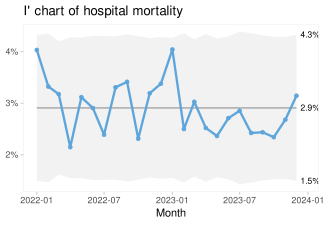
\includegraphics[width=0.5\linewidth]{_main_files/figure-latex/iprime-fig1-1} \includegraphics[width=0.5\linewidth]{_main_files/figure-latex/iprime-fig1-2} \caption{Comparing I' and P' charts}\label{fig:iprime-fig1}
\end{figure}

\subsection{Procedure for calculating centre line and control limits}\label{procedure-for-calculating-centre-line-and-control-limits}

We use the following symbols:

\begin{itemize}
\tightlist
\item
  \(n\) = numerators
\item
  \(d\) = denominators
\item
  \(o\) = number of data values (subgroups)
\item
  \(i\) = i\textsuperscript{th} data value
\end{itemize}

Values to plot:

\[
y = \frac{n}{d}
\]

Centre line:

\[
CL = \frac{\sum{n}}{\sum{d}}
\]

Standard deviation of i\textsuperscript{th} data point:

\[
s_i = \sqrt{\frac{\pi}{2}}\frac{\vert{}y_i-y_{i-1}\vert{}}{\sqrt{\frac{1}{d_i}+\frac{1}{d_{i-1}}}}
\]

Average standard deviation:

\[
\bar{s} = \frac{\sum{s}}{o}
\]

Control limits:

\[
\text{control limits} = CL \pm 3 \frac{\bar{s}}{\sqrt{d_i}}
\]

When subgroup sizes equals 1, the control limits simplify to: \(CL \pm 2.66\overline{MR}\) as in the original I chart.

As with the original I chart, qicharts2 screens the moving ranges of \(s_i\), removing ranges greater than the theoretical upper natural limit (= 3.2665) before calculating \(\bar{s}\).

\section{I' charts for measument data with variable subgroup sizes}\label{i-charts-for-measument-data-with-variable-subgroup-sizes}

Figure \ref{fig:iprime-fig1} demonstrates the use of an I' chart with count data. However, the I' chart was originally intended for use with measurement data where subgroup sizes vary. For example, due to privacy considerations, we may only have access to averaged patient data rather than individual records. Traditionally, such data would be plotted on an original I chart, but if the number of patients in each subgroup varies significantly, straight control limits may be suboptimal.

Figure \ref{fig:iprime-fig2} is an I chart of the monthly HbA1c averages from the \hyperref[diabetes-hba1c]{Diabetes HbA1c} dataset. Notice the data point above the upper control limit in April 2020 suggesting a special cause. However, when plotting aggregated measurement data, the I chart does not account for variations in subgroup size.

\begin{Shaded}
\begin{Highlighting}[]
\FunctionTok{qic}\NormalTok{(month, avg\_hba1c, }
    \AttributeTok{data  =}\NormalTok{ diabetes, }
    \AttributeTok{chart =} \StringTok{\textquotesingle{}i\textquotesingle{}}\NormalTok{,}
    \AttributeTok{title =} \ConstantTok{NULL}\NormalTok{,}
    \AttributeTok{ylab  =} \StringTok{\textquotesingle{}mmol / mol\textquotesingle{}}\NormalTok{,}
    \AttributeTok{xlab  =} \StringTok{\textquotesingle{}Month\textquotesingle{}}\NormalTok{)}
\end{Highlighting}
\end{Shaded}

\begin{figure}
\centering
\pandocbounded{\includesvg[keepaspectratio]{_main_files/figure-latex/iprime-fig2-1.svg}}
\caption{\label{fig:iprime-fig2}I chart of average HbA1c without denominator}
\end{figure}

The I' chart in Figure \ref{fig:iprime-fig3} takes the subgroup size (number of patients) into account and adjusts the control limits correspondingly.

\begin{Shaded}
\begin{Highlighting}[]
\FunctionTok{qic}\NormalTok{(month, avg\_hba1c }\SpecialCharTok{*}\NormalTok{ n, n, }
    \AttributeTok{data  =}\NormalTok{ diabetes, }
    \AttributeTok{chart =} \StringTok{\textquotesingle{}ip\textquotesingle{}}\NormalTok{,}
    \AttributeTok{title =} \ConstantTok{NULL}\NormalTok{,}
    \AttributeTok{ylab  =} \StringTok{\textquotesingle{}mmol / mol\textquotesingle{}}\NormalTok{,}
    \AttributeTok{xlab  =} \StringTok{\textquotesingle{}Month\textquotesingle{}}\NormalTok{)}
\end{Highlighting}
\end{Shaded}

\begin{figure}
\centering
\pandocbounded{\includesvg[keepaspectratio]{_main_files/figure-latex/iprime-fig3-1.svg}}
\caption{\label{fig:iprime-fig3}I prime chart of average HbA1c with denominator}
\end{figure}

April 2020 was the first month of lockdown during Covid-19 in Denmark, and the number of patients (the denominator) seen during this month was significantly lower than usual, which allowed for larger than usual common cause variation in measurements and consequently wider control limits this month. So, when the subgroup size is taken into account, the apparent special cause in Figure \ref{fig:iprime-fig2} is actually within the limits of the expected common cause variation.

Also, notice that the centre lines are a bit different (60.6 vs 60.3), because the I prime chart uses the weighted rather than the unweighted mean of the measurements.

Note that in order to plot the averages we need to multiply the numerators (avg\_hba1c, which are already averaged) by the denominators (n) to get the sum of individual measurements to use as the new numerator. Otherwise, the result would be a plot of averages of averages.

\section{One chart to rule them all?}\label{one-chart-to-rule-them-all}

The I' chart produces results that match the original I chart for individual measurements and P' and U' charts for proportion and count data.

If we accept Laney's claim that prime charts are valid -- or even better -- substitutes for their non-prime counterparts, it is tempting to conclude that the I' chart offers a universal solution to most, if not all, of our charting needs.

In conclusion, while the I' chart is a recent development, its versatility and ability to mimic the behaviour of traditional SPC charts make it a compelling alternative, that has the potential to streamline chart selection by serving as a single, robust option across various data types and scenarios. As the methodology continues to gain empirical support, the I' chart may well become the preferred tool for modern quality control.

\chapter{Funnel Plots for Categorical Subgroups}\label{funnel-plots-for-categorical-subgroups}

Funnel plots are SPC charts with categorical subgroups, which are often sorted after size to produce funnel shaped control limits. Funnel plots are useful for comparing indicator levels from different categories, for example complication rates from different hospitals.

Figure \ref{fig:funnel-fig0} compares the levels of some indicator across six organisational units. One unit (E) falls below the lower control limit, indicating that its data may reflect a fundamentally different process compared to the others.

\begin{figure}
\centering
\pandocbounded{\includesvg[keepaspectratio]{_main_files/figure-latex/funnel-fig0-1.svg}}
\caption{\label{fig:funnel-fig0}Funnel plot}
\end{figure}

Because funnel plots do not involve a natural time sequence, data points are not connected by lines, and run analysis is not applicable.

To demonstrate the construction of funnel plots we use data on urinary tract infections from the hospital\_infections dataset from qicharts2.

\begin{Shaded}
\begin{Highlighting}[]
\CommentTok{\# get urinary tract infections from hospital infections data}
\NormalTok{uti }\OtherTok{\textless{}{-}}\NormalTok{ hospital\_infections[hospital\_infections}\SpecialCharTok{$}\NormalTok{infection }\SpecialCharTok{==} \StringTok{\textquotesingle{}UTI\textquotesingle{}}\NormalTok{,]}

\CommentTok{\# plot U chart}
\FunctionTok{qic}\NormalTok{(month, n, days,}
    \AttributeTok{data     =}\NormalTok{ uti,}
    \AttributeTok{chart    =} \StringTok{\textquotesingle{}u\textquotesingle{}}\NormalTok{,}
    \AttributeTok{multiply =} \DecValTok{10000}\NormalTok{,}
    \AttributeTok{facets   =} \SpecialCharTok{\textasciitilde{}}\NormalTok{hospital,}
    \AttributeTok{ncol     =} \DecValTok{2}\NormalTok{,}
    \AttributeTok{title    =} \StringTok{\textquotesingle{}Hospital acquired urinary tract infections in six hospitals\textquotesingle{}}\NormalTok{,}
    \AttributeTok{ylab     =} \StringTok{\textquotesingle{}Infections per 10,000 risk days\textquotesingle{}}\NormalTok{,}
    \AttributeTok{xlab     =} \StringTok{\textquotesingle{}Month\textquotesingle{}}\NormalTok{)}
\end{Highlighting}
\end{Shaded}

\begin{figure}
\centering
\pandocbounded{\includesvg[keepaspectratio]{_main_files/figure-latex/funnel-fig1-1.svg}}
\caption{\label{fig:funnel-fig1}U chart of urinary tract infections}
\end{figure}

Figure \ref{fig:funnel-fig1} is a traditional U chart of infection rates in six hospital. There are signals of special cause variation in two hospitals (BOH, NOH), which makes direct comparison of infection rates between hospitals pointless -- it makes no sense to compare levels from data that are moving.

It is therefore important to select data from a recent and stable period of time before constructing funnel plots. In Figure \ref{fig:funnel-fig2} we have selected data from the most recent quarter and plotted them using hospital (rather than time) as the subgrouping variable.

\begin{Shaded}
\begin{Highlighting}[]
\CommentTok{\# filter data to latest quarter}
\NormalTok{uti\_2016q4 }\OtherTok{\textless{}{-}}\NormalTok{ uti[uti}\SpecialCharTok{$}\NormalTok{month }\SpecialCharTok{\textgreater{}=} \StringTok{\textquotesingle{}2016{-}10{-}01\textquotesingle{}}\NormalTok{, ]}

\CommentTok{\# plot "funnel" plot}
\FunctionTok{qic}\NormalTok{(hospital, n, days,}
    \AttributeTok{data     =}\NormalTok{ uti\_2016q4,}
    \AttributeTok{chart    =} \StringTok{\textquotesingle{}u\textquotesingle{}}\NormalTok{,}
    \AttributeTok{multiply =} \DecValTok{10000}\NormalTok{,}
    \AttributeTok{title    =} \StringTok{\textquotesingle{}Hospital acquired urinary tract infections in six hospitals\textquotesingle{}}\NormalTok{,}
    \AttributeTok{ylab     =} \StringTok{\textquotesingle{}Infections per 10,000 risk days\textquotesingle{}}\NormalTok{,}
    \AttributeTok{xlab     =} \StringTok{\textquotesingle{}Hospital\textquotesingle{}}\NormalTok{)}
\end{Highlighting}
\end{Shaded}

\begin{figure}
\centering
\pandocbounded{\includesvg[keepaspectratio]{_main_files/figure-latex/funnel-fig2-1.svg}}
\caption{\label{fig:funnel-fig2}Unordered `funnel' plot of urinary tract infections}
\end{figure}

By default the x-axis will be sorted alphabetically. To produce a funnel plot, we need to sort the subgroups by size as is shown in Figure \ref{fig:funnel-fig3}.

\begin{Shaded}
\begin{Highlighting}[]
\CommentTok{\# order hospitals by denominator (risk days) to produce funnel}
\FunctionTok{qic}\NormalTok{(}\FunctionTok{reorder}\NormalTok{(hospital, days), n, days,}
    \AttributeTok{data     =}\NormalTok{ uti\_2016q4,}
    \AttributeTok{chart    =} \StringTok{\textquotesingle{}u\textquotesingle{}}\NormalTok{,}
    \AttributeTok{multiply =} \DecValTok{10000}\NormalTok{,}
    \AttributeTok{title    =} \StringTok{\textquotesingle{}Hospital acquired urinary tract infections in six hospitals\textquotesingle{}}\NormalTok{,}
    \AttributeTok{ylab     =} \StringTok{\textquotesingle{}Infections per 10,000 risk days\textquotesingle{}}\NormalTok{,}
    \AttributeTok{xlab     =} \StringTok{\textquotesingle{}Hospital\textquotesingle{}}\NormalTok{)}
\end{Highlighting}
\end{Shaded}

\begin{figure}
\centering
\pandocbounded{\includesvg[keepaspectratio]{_main_files/figure-latex/funnel-fig3-1.svg}}
\caption{\label{fig:funnel-fig3}Ordered funnel plot of urinary tract infections}
\end{figure}

In summary, funnel plots are SPC charts with categorical subgroups. They are useful for comparing indicator levels across organisational units. To ensure valid comparisons, it is essential to use data from a recent, stable period that reflects only common cause variation before constructing a funnel plot.

\chapter{Pareto Charts for Ranking Problems}\label{pareto-charts-for-ranking-problems}

The Pareto chart, named after \href{https://en.wikipedia.org/wiki/Vilfredo_Pareto}{Vilfred Pareto}, was invented by \href{https://en.wikipedia.org/wiki/Joseph_M._Juran}{Joseph M. Juran} as a tool to identify the most important causes of a problem.

For this example, we use the dataset on \hyperref[adverse-events]{adverse events} causing harm to patients, collected using the Global Trigger Tool method (\citeproc{ref-plessen2012}{Plessen, Kodal, and Anhøj 2012}).

\begin{Shaded}
\begin{Highlighting}[]
\CommentTok{\# print structure of ae data}
\FunctionTok{str}\NormalTok{(ae)}
\end{Highlighting}
\end{Shaded}

\begin{verbatim}
## 'data.frame':    131 obs. of  2 variables:
##  $ severity: chr  "E" "F" "E" "F" ...
##  $ category: chr  "Pressure ulcer" "Gastrointestinal" "Infection" "Infection" ...
\end{verbatim}

The paretochart() function (from qicharts2) takes a categorical vector as argument and plots a Pareto chart as demonstrated in Figure \ref{fig:pareto-fig1}.

\begin{Shaded}
\begin{Highlighting}[]
\FunctionTok{paretochart}\NormalTok{(ae}\SpecialCharTok{$}\NormalTok{category)}
\end{Highlighting}
\end{Shaded}

\begin{figure}
\centering
\pandocbounded{\includesvg[keepaspectratio]{_main_files/figure-latex/pareto-fig1-1.svg}}
\caption{\label{fig:pareto-fig1}Pareto chart of patient harm.}
\end{figure}

The bars show the count in each category, and the curve shows the cumulated percentage over categories. Almost 80\% of harms come from 3 categories: gastrointestinal, infection, and procedure.

Figure \ref{fig:pareto-fig2} is a Pareto chart of harm severity demonstrating that nearly all events resulted in temporary harm (E-F).

\begin{Shaded}
\begin{Highlighting}[]
\FunctionTok{paretochart}\NormalTok{(ae}\SpecialCharTok{$}\NormalTok{severity)}
\end{Highlighting}
\end{Shaded}

\begin{figure}
\centering
\pandocbounded{\includesvg[keepaspectratio]{_main_files/figure-latex/pareto-fig2-1.svg}}
\caption{\label{fig:pareto-fig2}Pareto chart of harm severity: E-I, where E-F = temporary harm, G-H = permanent harm, and I = fatal harm.}
\end{figure}

The paretochart() function takes a character or factor vector, but often data have already been aggregated into tabular format:

\begin{Shaded}
\begin{Highlighting}[]
\NormalTok{ae.tbl}
\end{Highlighting}
\end{Shaded}

\begin{verbatim}
          category count
1             Fall     1
2 Gastrointestinal    40
3        Infection    34
4       Medication    18
5            Other     4
6   Pressure ulcer     5
7        Procedure    29
\end{verbatim}

To make a Pareto chart from tabular data, we first need to convert data back into a vector. This can be achieved with the rep() function repeating each category by its count:

\begin{Shaded}
\begin{Highlighting}[]
\CommentTok{\# make vector from counts}
\NormalTok{ae.cat }\OtherTok{\textless{}{-}} \FunctionTok{rep}\NormalTok{(ae.tbl}\SpecialCharTok{$}\NormalTok{category, ae.tbl}\SpecialCharTok{$}\NormalTok{count)}

\CommentTok{\# show first six rows of vector}
\FunctionTok{head}\NormalTok{(ae.cat)}
\end{Highlighting}
\end{Shaded}

\begin{verbatim}
## [1] Fall             Gastrointestinal Gastrointestinal Gastrointestinal
## [5] Gastrointestinal Gastrointestinal
## 7 Levels: Fall Gastrointestinal Infection Medication Other ... Procedure
\end{verbatim}

\begin{Shaded}
\begin{Highlighting}[]
\CommentTok{\# plot Pareto chart}
\FunctionTok{paretochart}\NormalTok{(ae.cat)}
\end{Highlighting}
\end{Shaded}

\begin{figure}
\centering
\pandocbounded{\includesvg[keepaspectratio]{_main_files/figure-latex/pareto-fig3-1.svg}}
\caption{\label{fig:pareto-fig3}Pareto chart constructed from tabular data.}
\end{figure}

In conclusion, the Pareto chart is useful for identifying the most common causes of a problem. Often most of the problems are caused by relatively few of the causes. In the example above eliminating gastrointestinal harm (most often obstipation) and hospital associated infections would more than half the rate of adverse events.

\part*{Part 5: Best Practices, Controversies, and Tips}\label{part-part-5-best-practices-controversies-and-tips}
\addcontentsline{toc}{part}{Part 5: Best Practices, Controversies, and Tips}

\chapter{Tips for Effective SPC Implementation}\label{tips-for-effective-spc-implementation}

\begin{itemize}
\tightlist
\item
  Automating production of SPC charts
\item
  Engaging stakeholders
\item
  Continuous monitoring and improvement.
\item
  Problems and challenges with SPC
\end{itemize}

\chapter{High Volume Data}\label{high-volume-data}

\chapter{Scaling Up Charts}\label{scaling-up-charts}

\begin{itemize}
\tightlist
\item
  technical issues
\item
  tabular charts
\item
  grids
\end{itemize}

\chapter{Common Pitfalls to Avoid}\label{common-pitfalls-to-avoid}

While SPC is a powerful framework for data-driven quality improvement, its effectiveness can be undermined by a range of common missteps. Misinterpretation of data, misuse of run and control charts, and faulty assumptions can lead to wasted effort or missed opportunities, and may ultimately erode trust in SPC itself.

This chapter outlines several common pitfalls to avoid.

\section{Data issues}\label{data-issues}

SPC charts are only as good as the data behind them. Poor data quality, including inaccurate measurements, inconsistent definitions or data collected under conditions that vary over time or between locations can significantly compromise their reliability.

How the subgroups are formed is especially important. Subgroups consist of the data elements included in each data point. The way data are sampled and grouped can greatly affect their ability to distinguish common cause variation from special cause variation. If subgrouping is not done properly, the SPC chart may generate false signals or obscure important ones. We have devoted a full chapter (\ref{subgrouping}) to \hyperref[subgrouping]{rational subgrouping}.

Time spend developing operational indicator definition and rational subgroups often yields significant returns. Investing effort upfront ensures that data are meaningful and comparable, enabling better decision-making.

\section{Signal fatigue from over-sensitive SPC rules}\label{signal-fatigue-from-over-sensitive-spc-rules}

Originally, control charts employed only one rule, the 3-sigma rule. However, to increase the chart's sensitivity to minor sustained shifts and other patterns of non-random variation, a plethora of supplementary rules have since been developed. To name a few, we have the Western Electric rules (four basic rules plus many more for specialised purposes), the Nelson rules (ten rules), and the Westgard rules (six rules). Most rules are based on identifying non-random patterns in the position of data points relative to the one-, two-, or three-sigma limits, each with different diagnostic properties.

Furthermore, several distinct sets of rules for runs analysis based on identifying non-random patterns relative the the centre line have been published (\citeproc{ref-anhoej2015}{Anhøj 2015}).

As discussed earlier in this book, it may seem tempting to apply as many rules as possible to increase the chance of detecting any signs of special cause variation. However, this strategy comes at a price. While additional rules do increase the sensitivity of SPC analysis, they also raise the risk of false alarms. This topic is further explored in Appendix \ref{diagnostics}, \hyperref[diagnostics]{Two Types of Errors When Using SPC}.

Apart from the risk of applying too many rules, the rules themselves may also be either overly sensitive or insufficiently sensitive. A prominent example is a commonly used set of runs rules -- including four tests for trends, shifts, and too many or too few runs respectively -- adopted by many healthcare organisations (\citeproc{ref-provost2011}{Provost and Murray 2011}; \citeproc{ref-perla2011}{Perla, Provost, and Murray 2011}). This particular set has been shown to produce a very high rate of false signals. For instance, in a run chart with 24 data points, the expected false positive rate is close to 50\% (\citeproc{ref-anhoej2015}{Anhøj 2015}). The main contributor appears to be the trend rule -- defined as five or more consecutive data points all increasing or decreasing. Short trends like this are very common, even in sequences of purely random numbers. Moreover, trend rules in general have been thoroughly studied and found to be, at best, unhelpful and, at worst, misleading (\citeproc{ref-davis1988}{Davis and Woodall 1988}).

To make matters worse, some practitioners deliberately tighten control limits in an attempt to increase the sensitivity of the sigma rule. This behaviour often stems from another common mistake: using the overall standard deviation to calculate control limits (\citeproc{ref-wheeler2010}{Wheeler 2010}, \citeproc{ref-wheeler2016}{2016}). As emphasised repeatedly throughout this book, the overall variation is not appropriate for this purpose, as it includes both common cause and special cause variation -- ultimately inflating the control limits. Inflated limits can, in turn, prompt misguided attempts to narrow them artificially. Instead, control limits, set at ±3-sigma from the centre line, should be based on the estimated within-subgroup standard deviation from rationally formed subgroups. This approach captures common cause variation and provides a sound basis for meaningful process monitoring and improvement.

To avoid signal fatigue -- which, at best, results in wasted effort from chasing false signals -- we recommend that practitioners select their rules carefully, focusing on capturing patterns that are most likely to signal special cause variation in their specific context. The three rules suggested in this book -- the two runs rules and the 3-sigma rule -- have been deliberately designed to detect patterns indicative of one or more of the types of variation most commonly encountered in healthcare improvement: freaks, shifts, trends or cycles, while keeping acceptable false alarm rates.

\section{Confusing the voice of the customer with the voice of the process}\label{confusing-the-voice-of-the-customer-with-the-voice-of-the-process}

``Hearing voices'' is essential to effective SPC implementation. Two voices demand close attention: the voice of the customer and the voice of the process. Both are important, but confusing one for the other can lead to misguided actions, wasted effort, and poor decision-making.

The voice of the customer refers to the expected or desired outcomes of the process, while the voice of the process reflects its actual capability and stability regardless of what the customer wants.

The voice of the customer is often expressed through specification limits that define the desired level of outcomes. These limits may take the form of an upper or lower acceptance threshold, or an interval specifying the acceptable range for a given outcome. For example, based on literature reviews or results from comparable units, it may be determined that an acute caesarean section should be completed within 30 minutes of the decision to operate. Any procedure taking longer than this would be considered unacceptable.

If we listen only to the voice of the customer, it may be tempting to treat any caesarean section taking longer than 30 minutes as a special cause -- and perhaps even initiate a root cause analysis in each case. However, without also considering the voice of the process -- which tells us whether the process is stable and what it is actually capable of, as indicated by the control limits -- such an approach is flawed.

Unacceptable outcomes may well arise from highly stable and predictable processes -- and conversely, acceptable outcomes may result from unstable ones. Before taking action based on specific outcomes, we must first determine whether they are the result of common cause or special cause variation. This distinction is crucial, as each type of variation calls for a fundamentally different approach to improvement.

As detailed in Chapter \ref{variation}, \hyperref[variation]{Understanding Variation}, addressing common cause variation requires a thorough redesign of the entire process, while addressing special cause variation involves identifying the root causes of the special cause(s) and either eliminating or reinforcing them, depending on whether they are undesirable or beneficial.

The long-term goal of any improvement initiative is to establish stable processes that consistently deliver acceptable results.

The two voices and the corresponding four appropriate actions are summarised in the table below:

\begin{longtable}[]{@{}
  >{\raggedright\arraybackslash}p{(\linewidth - 4\tabcolsep) * \real{0.2308}}
  >{\raggedright\arraybackslash}p{(\linewidth - 4\tabcolsep) * \real{0.3750}}
  >{\raggedright\arraybackslash}p{(\linewidth - 4\tabcolsep) * \real{0.3942}}@{}}
\caption{The interplay between the voice of the customer and the voice of the process, with the four appropriate actions for each scenario.}\tabularnewline
\toprule\noalign{}
\begin{minipage}[b]{\linewidth}\raggedright
\end{minipage} & \begin{minipage}[b]{\linewidth}\raggedright
\textbf{Process Stable}
\end{minipage} & \begin{minipage}[b]{\linewidth}\raggedright
\textbf{Process Unstable}
\end{minipage} \\
\midrule\noalign{}
\endfirsthead
\toprule\noalign{}
\begin{minipage}[b]{\linewidth}\raggedright
\end{minipage} & \begin{minipage}[b]{\linewidth}\raggedright
\textbf{Process Stable}
\end{minipage} & \begin{minipage}[b]{\linewidth}\raggedright
\textbf{Process Unstable}
\end{minipage} \\
\midrule\noalign{}
\endhead
\bottomrule\noalign{}
\endlastfoot
\textbf{Customer Satisfied} & OK -- hands off and continue to monitor & Trouble ahead -- stabilise the process \\
\textbf{Customer Unsatisfied} & Trouble now -- revise the process & Chaos -- revise and stabilise the process \\
\end{longtable}

\section{Automatic rephasing}\label{automatic-rephasing}

Rephasing involves splitting an SPC chart to recalculate the centre line and control limits after a sustained shift has been identified.

Figure \ref{fig:pitfalls-fig1} shows the number of hospital infections (C. diff.) before and after an intervention, which began after month 24.

\begin{Shaded}
\begin{Highlighting}[]
\FunctionTok{qic}\NormalTok{(month, n,}
    \AttributeTok{data  =}\NormalTok{ cdi,}
    \AttributeTok{chart =} \StringTok{\textquotesingle{}c\textquotesingle{}}\NormalTok{,}
    \AttributeTok{title =} \StringTok{\textquotesingle{}Hospital associated C. diff.{-}infections\textquotesingle{}}\NormalTok{,}
    \AttributeTok{ylab  =} \StringTok{\textquotesingle{}Count\textquotesingle{}}\NormalTok{,}
    \AttributeTok{xlab  =} \StringTok{\textquotesingle{}Month\textquotesingle{}}\NormalTok{)}
\end{Highlighting}
\end{Shaded}

\begin{figure}
\centering
\pandocbounded{\includesvg[keepaspectratio]{_main_files/figure-latex/pitfalls-fig1-1.svg}}
\caption{\label{fig:pitfalls-fig1}Hospital infections.}
\end{figure}

Figure \ref{fig:pitfalls-fig2} has been rephased following the start of the intervention and the subsequent shift. This correctly distinguishes two distinct periods, each with stable but differing levels of infections.

\begin{Shaded}
\begin{Highlighting}[]
\FunctionTok{qic}\NormalTok{(month, n,}
    \AttributeTok{data  =}\NormalTok{ cdi,}
    \AttributeTok{chart =} \StringTok{\textquotesingle{}c\textquotesingle{}}\NormalTok{,}
    \AttributeTok{part  =}\NormalTok{ period,}
    \AttributeTok{title =} \StringTok{\textquotesingle{}Hospital associated C. diff.{-}infections\textquotesingle{}}\NormalTok{,}
    \AttributeTok{ylab  =} \StringTok{\textquotesingle{}Count\textquotesingle{}}\NormalTok{,}
    \AttributeTok{xlab  =} \StringTok{\textquotesingle{}Month\textquotesingle{}}\NormalTok{)}
\end{Highlighting}
\end{Shaded}

\begin{figure}
\centering
\pandocbounded{\includesvg[keepaspectratio]{_main_files/figure-latex/pitfalls-fig2-1.svg}}
\caption{\label{fig:pitfalls-fig2}Hospital infections -- rephasing done right!}
\end{figure}

Automatic rephasing is when the centre line and control limits are recalculated \emph{automatically} after the software detects a shift -- typically triggered by a prolonged run of data points on one side of the centre line. Some software packages perform automatic rephasing by default (Reading et al. (\citeproc{ref-reading2021}{2021})).

Figure \ref{fig:pitfalls-fig3} has been automatically rephased following detection of the shift. Coincidentally, the run that signalled the shift began three months prior to the intervention. However, these months should correctly be considered part of the baseline period. As a result, the control limits and centre lines do not accurately reflect the distinct before-and-after periods. The centre lines are inflated, and a freak data point falsely suggests instability during the baseline period.

\begin{Shaded}
\begin{Highlighting}[]
\FunctionTok{qic}\NormalTok{(month, n,}
    \AttributeTok{data        =}\NormalTok{ cdi,}
    \AttributeTok{chart       =} \StringTok{\textquotesingle{}c\textquotesingle{}}\NormalTok{,}
    \AttributeTok{part        =} \DecValTok{22}\NormalTok{,}
    \AttributeTok{part.labels =} \FunctionTok{c}\NormalTok{(}\StringTok{\textquotesingle{}pre\textquotesingle{}}\NormalTok{, }\StringTok{\textquotesingle{}post\textquotesingle{}}\NormalTok{),}
    \AttributeTok{title       =} \StringTok{\textquotesingle{}Hospital associated C. diff.{-}infections\textquotesingle{}}\NormalTok{,}
    \AttributeTok{ylab        =} \StringTok{\textquotesingle{}Count\textquotesingle{}}\NormalTok{,}
    \AttributeTok{xlab        =} \StringTok{\textquotesingle{}Month\textquotesingle{}}\NormalTok{)}
\end{Highlighting}
\end{Shaded}

\begin{figure}
\centering
\pandocbounded{\includesvg[keepaspectratio]{_main_files/figure-latex/pitfalls-fig3-1.svg}}
\caption{\label{fig:pitfalls-fig3}Hospital infections -- rephasing done wrong!}
\end{figure}

We strongly discourage the use of automatic rephasing, as it can lead to misleading interpretations of process stability. By automating shift detection, automatic rephasing effectively removes the essential human insight into the process. Therefore, rephasing should be a deliberate decision made by individuals with a thorough understanding of the process and any associated interventions.

Rephasing \emph{may} be appropriate when the following conditions are met:

\begin{itemize}
\tightlist
\item
  there is a sustained shift in data,
\item
  the reason for the shift is known,
\item
  the shift is in the desired direction, and
\item
  the shift is expected to continue.
\end{itemize}

If any of these conditions is not met, we should rather seek to understand the nature and causes of any shift, following the strategy outlined in Chapter \ref{using}, \hyperref[using]{Using SPC in Healthcare}.

\section{The control chart vs run chart debate}\label{the-control-chart-vs-run-chart-debate}

It is a common and persistent misconception that control charts are inherently superior to run charts in detecting special cause variation (e.g. Carey (\citeproc{ref-carey2002b}{2002})). Similarly, run charts and control charts are often viewed as fundamentally different methods, warranting distinct terminologies (e.g. Perla, Provost, and Murray (\citeproc{ref-perla2011}{2011})). We disagree with both notions.

We refer to run charts and control charts collectively as SPC charts -- time series charts that use statistical tests to detect signs of special cause variation. These tests -- known as rules -- employ various techniques to identify patterns in data that are unlikely to arise in stable (i.e., purely random) processes.

All SPC rules share a common basis: they rely on the position of data points relative to the process centre and/or process spread. For a detailed discussion of these concepts, see Appendix \ref{diagnostics}, \hyperref[stat-concepts]{Basic Statistical Concepts}.

Traditionally, control charts use rules based on sigma limits, while run charts apply rules based on the centre line. However, combining rules based on both centre and spread -- as we advocate throughout this book -- is not a new practice. Consider Rule \#4 of the Western Electric rules -- a run of eight or more consecutive data points on the same side of the centre line. This rule, which is independent of sigma limits, is grounded in the same statistical principle as the two runs rules for unusually long or few runs.

Thus, run charts and control charts are two sides of the same coin, with the key difference being the presence or absence of control limits. These limits serve to quickly signal sudden, significant shifts in the data and to provide a visual representation of natural process variation. Runs analysis -- using rules for unusually long or few runs (or crossings) -- is more effective than control limits for detecting minor to moderate \emph{sustained} shifts or trends in data. Combining these two principles offers the best of both worlds.

Nonetheless, standalone run charts present some advantages over control charts. A key benefit is that run charts are a lot easier to construct than control charts using pen and paper only: plot the dots, and draw a horizontal line that splits data in half.

Additionally, using the median rather than the mean as the centre line effectively divides the data symmetrically, making the chart largely independent of distributional assumptions and less prone to misapplication. The latter being particularly important i healthcare were many practitioners lack formal statistical training.

Finally, because runs analysis is most effective for detecting minor to moderate sustained shifts, which is ultimately what we seek when aiming to improve processes, run charts may be all that is needed during the improvement phase. Once a satisfactory level of improvement has been achieved, control limits can be added -- along with switching to the mean as the centre line -- to monitor process stability and quickly detect sudden larger, and possibly transient, shifts in the data.

\section{Assuming a one-to-one link between PDSA cycles and data points}\label{assuming-a-one-to-one-link-between-pdsa-cycles-and-data-points}

While this issue may not result in faulty SPC analyses, it often causes confusion among practitioners. SPC is frequently taught alongside improvement work using PDSA cycles, which can lead to the mistaken belief that there must be a one-to-one correspondence between PDSA cycles and data points on an SPC chart. In other words, any detected freak, shift or trend is assumed to be directly linked to specific PDSA cycles testing particular actions. Conversely, the absence of signals may be misinterpreted as evidence that a PDSA cycle has failed.

This is, however, far from always the case. PDSA cycles tend to run quickly (minutes, hours, days), while SPC charts reflect changes more slowly (days, weeks, months).

Therefore, it is important for practitioners to recognise that SPC charts and PDSA cycles operate on different timescales and serve complementary but distinct purposes. SPC should be used as a broader monitoring tool to observe trends and shifts over time, while PDSA cycles focus on rapid, iterative testing and learning. Understanding this distinction helps ensure more effective use of both methods in quality improvement efforts.

\chapter{The Forgotten Art of Rational Subgrouping}\label{subgrouping}

A subgroup consists of the data elements that make up a single data point, for example, the waiting times used to calculate the average waiting time for a particular period.

Rational subgrouping is the intentional and intelligent sampling and grouping of data into data points for SPC charts with the aim of maximising the chances of detecting special cause variation while minimising the risk of false alarms. In other words, rational subgrouping is all about maximising the signal-to-noise ratio.

A rational subgroup consists of a set of measurements or counts that are:

\begin{itemize}
\tightlist
\item
  produced under conditions that are as similar as possible,
\item
  taken close together in time and space, and
\item
  likely to show only common cause variation.
\end{itemize}

The underlying logic is that when subgroups are rationally formed, variation within subgroups reflects common cause variation, whereas variation between subgroups that exceeds what is expected from within-subgroup variation indicates the presence of special causes.

In our experience -- particularly in healthcare -- rational subgrouping is something of a forgotten art. We often rely on whatever data are readily available, which are frequently pre-aggregated into monthly, quarterly, or even yearly time periods for administrative purposes rather than for quality improvement. This practice often leads to suboptimal use of data for driving improvement.

\section{Too large subgroups --- masking meaningful signals}\label{too-large-subgroups-masking-meaningful-signals}

A common mistake is forming subgroups across overly broad spans of time or space (e.g.~organisational units), which blends common and special cause variation and effectively obscures the latter.

As an example, figures \ref{fig:subgrouping-fig1} and \ref{fig:subgrouping-fig2} display the number of C. diff. infections subgrouped by monthly and two-monthly periods respectively.

\begin{Shaded}
\begin{Highlighting}[]
\FunctionTok{qic}\NormalTok{(month, infections, }
    \AttributeTok{data  =}\NormalTok{ cdiff, }
    \AttributeTok{chart =} \StringTok{\textquotesingle{}c\textquotesingle{}}\NormalTok{,}
    \AttributeTok{title =} \StringTok{\textquotesingle{}C. diff. infections\textquotesingle{}}\NormalTok{,}
    \AttributeTok{ylab  =} \StringTok{\textquotesingle{}Count\textquotesingle{}}\NormalTok{,}
    \AttributeTok{xlab  =} \StringTok{\textquotesingle{}Months\textquotesingle{}}\NormalTok{)}
\end{Highlighting}
\end{Shaded}

\begin{figure}
\centering
\pandocbounded{\includesvg[keepaspectratio]{_main_files/figure-latex/subgrouping-fig1-1.svg}}
\caption{\label{fig:subgrouping-fig1}Monthly C. diff. infections.}
\end{figure}

\begin{Shaded}
\begin{Highlighting}[]
\FunctionTok{qic}\NormalTok{(month, infections, }
    \AttributeTok{data     =}\NormalTok{ cdiff, }
    \AttributeTok{chart    =} \StringTok{\textquotesingle{}c\textquotesingle{}}\NormalTok{,}
    \AttributeTok{x.period =} \StringTok{\textquotesingle{}2 months\textquotesingle{}}\NormalTok{,}
    \AttributeTok{title    =} \StringTok{\textquotesingle{}C. diff. infections\textquotesingle{}}\NormalTok{,}
    \AttributeTok{ylab     =} \StringTok{\textquotesingle{}Count\textquotesingle{}}\NormalTok{,}
    \AttributeTok{xlab     =} \StringTok{\textquotesingle{}Two{-}months\textquotesingle{}}\NormalTok{)}
\end{Highlighting}
\end{Shaded}

\begin{figure}
\centering
\pandocbounded{\includesvg[keepaspectratio]{_main_files/figure-latex/subgrouping-fig2-1.svg}}
\caption{\label{fig:subgrouping-fig2}Two-monthly C. diff. infections.}
\end{figure}

By using larger subgoups, as shown in Figure \ref{fig:subgrouping-fig2}, we effectively mask the two signals -- a freak value and a sustained shift -- that suggest the process is trending downwards. Clearly, if the trend continues, it will eventually become apparent even with two-monthly data, but it will inevitably take longer to detect delaying any potential learning or intervention.

To avoid over-aggregating data by using excessively large subgroups, we need to record data at a temporal resolution that, at minimum, matches the expected rate of change we are trying to detect. High-resolution data can always be aggregated to a lower resolution if suitable (or necessary), but low-resolution data cannot be further resolved.

Note that the qic() function from qicharts2 includes an argument, x.period, which allows us to aggregate data into larger subgroups as demonstrated in the code producing Figure \ref{fig:subgrouping-fig2}.

\section{Too small subgroups --- revealing unimportant noise}\label{too-small-subgroups-revealing-unimportant-noise}

A less common -- but equally important -- mistake is to form subgroups that are too small, which fail to capture natural process noise and thus misinterpret it as special cause variation..

Imagine stepping on a scale three times each morning for a couple of weeks, and plotting the results on an X-bar chart, using the within-subgroup (within-day) variation as the basis for calculating control limits.

Figure \ref{fig:subgroups-fig3} illustrates this with simulated data. As expected, the variation within each daily subgroup is very low, while the variation between subgroups is noticeably higher suggesting that our body weight is highly unstable from day to day. However, this difference between within- and between-subgroup variation merely reflects natural physiological fluctuations and is irrelevant to our goal of monitoring long-term body weight trends.

\begin{Shaded}
\begin{Highlighting}[]
\CommentTok{\# lock random number generator for reproducibility}
\FunctionTok{set.seed}\NormalTok{(}\DecValTok{5}\NormalTok{)}

\CommentTok{\# subgroups, 12 subgroups of three values}
\NormalTok{x }\OtherTok{\textless{}{-}} \FunctionTok{rep}\NormalTok{(}\DecValTok{1}\SpecialCharTok{:}\DecValTok{12}\NormalTok{, }\AttributeTok{each =} \DecValTok{3}\NormalTok{)}

\CommentTok{\# random values, each repeated three times}
\NormalTok{y }\OtherTok{\textless{}{-}} \FunctionTok{rep}\NormalTok{(}\FunctionTok{rnorm}\NormalTok{(}\DecValTok{12}\NormalTok{, }\AttributeTok{mean =} \DecValTok{80}\NormalTok{, }\AttributeTok{sd =} \FloatTok{0.5}\NormalTok{), }\AttributeTok{each =} \DecValTok{3}\NormalTok{)}

\CommentTok{\# add a bit of random noise within subgroups}
\NormalTok{y }\OtherTok{\textless{}{-}} \FunctionTok{jitter}\NormalTok{(y, }\AttributeTok{amount =} \FloatTok{0.2}\NormalTok{)}

\CommentTok{\# plot Xbar{-}chart}
\FunctionTok{qic}\NormalTok{(x, y, }\AttributeTok{chart =} \StringTok{\textquotesingle{}xbar\textquotesingle{}}\NormalTok{)}
\end{Highlighting}
\end{Shaded}

\begin{figure}
\centering
\pandocbounded{\includesvg[keepaspectratio]{_main_files/figure-latex/subgroups-fig3-1.svg}}
\caption{\label{fig:subgroups-fig3}Xbar-chart from too small subgroups.}
\end{figure}

A better strategy would be to plot data using an I-chart of the daily averages. The I-chart uses the moving range between successive subgroups as a basis for calculating control limits, which is -- in this case -- a much better representation of the day-to-day variation, which is really what we want to monitor.

\begin{Shaded}
\begin{Highlighting}[]
\FunctionTok{qic}\NormalTok{(x, y, }\AttributeTok{chart =} \StringTok{\textquotesingle{}i\textquotesingle{}}\NormalTok{)}
\end{Highlighting}
\end{Shaded}

\begin{verbatim}
## Subgroup size > 1. Data have been aggregated using mean().
\end{verbatim}

\begin{figure}
\centering
\pandocbounded{\includesvg[keepaspectratio]{_main_files/figure-latex/subgroups-fig4-1.svg}}
\caption{\label{fig:subgroups-fig4}I-chart of average daily body weight.}
\end{figure}

Alternatively, we could devise a different sampling plan that produces subgroups better representing the process of interest -- for example, using weekly averages of daily measurements as subgroups.

Depending on our goal, different subgrouping strategies may be appropriate. If the aim is to monitor and maintain a stable body weight, weekly subgroups may be sufficient. However, if the objective is to support a weight-reduction plan expecting significant weekly decreases, daily measurements could prove more useful.

\section{Striking the balance}\label{striking-the-balance}

As the chapter title suggests, rational subgrouping is as much an art as it is a science. In fact, it remains one of the more complex and unresolved challenges in statistical process control: to understand a process, we need rational subgroups -- but to form rational subgroups, we need to understand the process.

In practice, we frequently need to try multiple approaches to subgrouping our data -- experimenting with different timeframes, organisational units or other dimensions -- before finding an approach that meaningfully reflects the underlying process behaviour.

That said, in healthcare -- in contrast to the production industry -- there is often far less flexibility to tailor data collection to the requirements of SPC. In a production setting, where outputs are counted in the thousands and inputs are largely under control, it is possible to design highly specific sampling plans aligned to precise time intervals and structured across machinery, personnel and organisational units.

In healthcare, by contrast, the smallest meaningful unit is typically the individual patient or procedure, situated within a specific organisational context or clinical pathway. Outcomes are shaped by a complex interplay of factors -- including clinical complexity, social determinants, people, and system-level variation. Unlike components in a production process, this variability cannot be standardised or controlled with the same degree of precision.

However, that does not mean that we should not care about rational subgrouping. Although we may have limited control over input variation we can still design sampling strategies that aim to minimise the impact of these sources of variation by carefully selecting patient groups, clinical pathways, organisational units and time periods that reliably reflect the processes we aim to understand. Doing so helps preserve an optimal signal-to-noise ratio, enhancing our ability to detect meaningful changes.

\section{A practical approach for rational subgrouping}\label{a-practical-approach-for-rational-subgrouping}

There is no single ideal procedure for designing rational subgroups. As noted previously, this often requires an iterative process involving trial and error: Plan-Do-Study-Act.

Here are a few suggestions to consider when designing rational subgroups:

\begin{enumerate}
\def\labelenumi{\arabic{enumi}.}
\item
  Consult individuals with expert knowledge of the process in question -- rational subgrouping is a collaborative effort, not merely a statistical exercise.
\item
  Develop a detailed model of the process -- including inputs, outputs, and factors that may influence either.
\item
  Consider whether your objective is monitoring or improving the process.
\item
  Consider the level of organisational granularity at which the data should be analysed, and whether aggregation or stratification is appropriate.
\item
  Consider the rate of change you aim to detect.
\item
  Choose a timeframe for sampling that is shorter than the expected rate of change.
\item
  For count data, select a timeframe for sampling long enough to capture at least five events or cases (numerator); for proportion data, ensure there are at least five additional opportunities (denominator).
\item
  Remain flexible and open to revising your sampling strategy as new insights emerge.
\end{enumerate}

Note that decisions about temporal and organisational granularity (\#4--6) may conflict with the requirement for sufficiently large subgroups (\#7) to ensure meaningful analysis. In such cases, it may be necessary to compromise or explore alternative methods to monitor the processes of interest -- for example using different indicators or charts better suited for rare events.

\section{Rational subgrouping ``in short''}\label{rational-subgrouping-in-short}

Despite the section header, there is no truly concise way to explain rational subgrouping. It is one of the most challenging aspects of SPC to understand and apply correctly -- not least because there is no single recipe for getting it right.

Still, there is no excuse -- getting rational subgrouping right is what separates meaningful SPC charts from those that mislead or fall short.

\part*{Part 6: Conclusion and Final Thoughts}\label{part-part-6-conclusion-and-final-thoughts}
\addcontentsline{toc}{part}{Part 6: Conclusion and Final Thoughts}

\appendix


\chapter{Data Sets}\label{data-sets}

Datasets for this book are provided as comma separated values (csv) in text files. For details on how to read data from csv-files, see the \hyperref[importing-data-from-text-files]{Importing data from text files} in Appendix \ref{r-notes}.

\subsection*{Adverse Events}\label{adverse-events}
\addcontentsline{toc}{subsection}{Adverse Events}

Patient harm found with the Global Trigger Tool

File: adverse\_events.csv

Variables:

\begin{itemize}
\tightlist
\item
  severity (character): Harm severity: E = minor transient, I = fatal
\item
  category (character): Harm category
\end{itemize}

\subsection*{Bacteremia}\label{bacteremia}
\addcontentsline{toc}{subsection}{Bacteremia}

Hospital acquired and all cause bacteremias and 30 days mortality

File: bacteremia.csv

Variables:

\begin{itemize}
\tightlist
\item
  month (date): month of infection
\item
  ha\_infections (numeric): number of hospital acquired infections
\item
  risk\_days (numeric): number of patient days without infection
\item
  deaths (numeric): 30-day mortality after all-cause infection
\item
  patients (numeric): number of patients with all-cause infection
\end{itemize}

\subsection*{Blood pressure}\label{blood-pressure}
\addcontentsline{toc}{subsection}{Blood pressure}

Daily measurements of blood pressure and resting pulse.

File: blood\_pressure.csv

Variables:

\begin{itemize}
\tightlist
\item
  date (date): date of measurement
\item
  systolic (numeric): systolic blood pressure (mm Hg)
\item
  diastolic (numeric): diastolic blood pressure (mm Hg)
\item
  pulse (numeric): resting pulse (beats per minute)
\end{itemize}

\subsection*{Clostridioides difficile infections}\label{clostridioides-difficile-infections}
\addcontentsline{toc}{subsection}{Clostridioides difficile infections}

Hospital acquired C. diff. infections

File: cdiff.csv

Variables:

\begin{itemize}
\tightlist
\item
  month (date): first day of month
\item
  cases (numeric): number of cases
\item
  risk\_days (numeric): number of patient days without infection
\end{itemize}

\subsection*{Ceasearian section delay}\label{ceasearian-section-delay}
\addcontentsline{toc}{subsection}{Ceasearian section delay}

Time to grade 2 C-section

File: csection\_delay.csv

Variables:

\begin{itemize}
\tightlist
\item
  datetime (datetime): date and time of delivery
\item
  month (date): first day of month
\item
  delay (numeric): time in minutes between decision and delivery
\end{itemize}

\subsection*{Diabetes HbA1c}\label{diabetes-hba1c}
\addcontentsline{toc}{subsection}{Diabetes HbA1c}

HbA1c measurements in children with diabetes

File: diabetes\_hba1c.csv

Variables:

\begin{itemize}
\tightlist
\item
  month (date): month of measurements
\item
  avg\_hba1c (numeric): average of HbA1c measurements
\item
  n (integer): number of patients who visited the clinic
\end{itemize}

\subsection*{Emergency admission mortality}\label{emergency-admission-mortality}
\addcontentsline{toc}{subsection}{Emergency admission mortality}

7-day mortality after emergency admission

File: emergency\_admission.csv

Variables:

\begin{itemize}
\tightlist
\item
  month (date): first day of month
\item
  deaths (numeric): number of deaths within 7 days after emergency admission
\item
  admissions (numeric): number of emergency admissions
\end{itemize}

\subsection*{On-time CT}\label{on-time-ct}
\addcontentsline{toc}{subsection}{On-time CT}

Patients with acute abdomen CT scanned within 3 hours after arrival

File: ontime\_ct.csv

Variables:

\begin{itemize}
\tightlist
\item
  month (date): first day of month
\item
  ct\_on\_time (numeric): number of patients scanned within 3 hours
\item
  cases (numeric): number of patients with acute abdomen
\end{itemize}

\subsection*{Radiation doses}\label{radiation-doses}
\addcontentsline{toc}{subsection}{Radiation doses}

Radiation doses used for renography

File: renography\_doses.csv

Variables:

\begin{itemize}
\tightlist
\item
  date (date): date of renography
\item
  week (date): first day of week
\item
  dose (numeric): radiation dose in megabequerel
\end{itemize}

\subsection*{Robson group 1 births}\label{robson-group-1-births}
\addcontentsline{toc}{subsection}{Robson group 1 births}

Outcomes and complications of Robson group 1 births: first time
pregnancy, single baby, head first, gestational age at least 37 weeks.

File: robson1\_births.csv

Variables:

\begin{itemize}
\tightlist
\item
  datetime (datetime): data and time of birth
\item
  biweek (date): first day of biweekly period
\item
  csect (logical): delivery by C-section
\item
  cup (logical): delivery by vacuum extraction
\item
  sex (character): sex of baby
\item
  length (numeric): baby length in cm
\item
  weight (numeric): baby weight in kg
\item
  apgar (numeric): apgar score at 5 minutes
\item
  ph (numeric): arterial umbilical chord pH
\item
  asphyxia (logical): ph \textless{} 7 or missing ph and apgar \textless{} 7
\end{itemize}

\chapter{Basic Statistical Concepts}\label{stat-concepts}

Understanding data is the cornerstone of effective decision-making in any quality improvement context. While this chapter is not intended as a comprehensive statistical tutorial, it introduces key concepts related to data types, basic statistical summaries, and visualisation techniques that support meaningful application of appropriate SPC charts and help ensure that valid data-driven conclusions can be drawn.

\section{Data types}\label{data-types}

Data can be classified into several types, with the most common being categorical and numerical data.

\subsection{Categorical data}\label{categorical-data}

Categorical data, also known as qualitative data, represent characteristics that cannot be meaningfully measured on a numerical scale, for example {[}red, green, blue{]}, {[}medicine, surgery, psychiatry{]} or {[}low, medium, high{]}. Categorical data cannot be directly analysed using arithmetic operations -- what is the sum of red, green and blue, for example?

Categorical data can be divided into:

\begin{itemize}
\item
  Nominal data: Categories without a natural order, e.g.~{[}red, green, blue{]} or {[}medicine, surgery, psychiatry{]}.
\item
  Ordinal data: Categories with a meaningful order, but without consistent intervals between them, e.g.~{[}low \textless{} medium \textless{} high{]}.
\end{itemize}

If categorical data consist of only two possible values -- such as yes/no, true/false or dead/alive -- they are referred to as binary or binomial data.

Categorical data can be transformed into numerical form by counting the number of observations in each category. In some (rare) cases, it may be appropriate to assign numerical values to ordinal data, such as school grades, thereby enabling the use of arithmetic operations. However, we should be careful not to impose numerical values on any ordinal data unless the intervals are consistent and well-defined. It may be tempting to converts, for instance, cancer stages {[}I, II, III{]} into numbers {[}1, 2, 3{]}. But this will only make sense, if cancer stage II is exactly twice as severe as stage I, and stage III three times as severe.

Note that some categorical data -- such as postal codes, insurance numbers and phone numbers -- may appear numerical but are actually categorical. To identify such cases, ask whether it makes sense to calculate a sum or an average. If not, the values should be treated as categories rather than numbers.

\subsection{Numerical data}\label{numerical-data}

Numerical data, also known as quantitative data, consist of values that represent measurable quantities. These data can be meaningfully analysed using arithmetic operations such as addition or subtraction.

Numerical data fall in two main subtypes:

\begin{itemize}
\item
  Discrete data: Distinct, separate values that result from counting and are always expressed as whole numbers (including zero). Examples include number of pregnancies, pressure ulcers and hospital admissions.
\item
  Continuous data: Values obtained through measurement that can take on any value within a given range, including decimals, fractions and negative numbers. Examples include height, weight, waiting time and blood pressure.
\end{itemize}

Just as categorical data can be converted into numbers through counting, numerical data can be transformed into categories by grouping values into defined ranges --- for example, converting exact blood pressure readings into hypertension categories such as normal, elevated, stage 1 hypertension, and stage 2 hypertension.

\section{Summarising categorical data}\label{summarising-categorical-data}

In this section we use the \hyperref[adverse-events]{Adverse events} dataset assigned to the variable ae.

As mentioned, categorical data are most commonly summarised by counting the number of observations in each category, typically presented as frequencies or proportions (or percentages). In R, this can be easily done using the table() function.

\begin{Shaded}
\begin{Highlighting}[]
\CommentTok{\# count number of adverse events in each category}
\NormalTok{(ae.tbl }\OtherTok{\textless{}{-}} \FunctionTok{table}\NormalTok{(ae}\SpecialCharTok{$}\NormalTok{category))}
\end{Highlighting}
\end{Shaded}

\begin{verbatim}
## 
##             Fall Gastrointestinal        Infection       Medication 
##                1               40               34               18 
##            Other   Pressure ulcer        Procedure 
##                4                5               29
\end{verbatim}

A useful visualisation of categorical data is the bar chart displaying either the frequencies or proportions in each category:

\begin{Shaded}
\begin{Highlighting}[]
\CommentTok{\# plot frequencies}
\FunctionTok{barplot}\NormalTok{(ae.tbl)}
\end{Highlighting}
\end{Shaded}

\begin{figure}
\centering
\pandocbounded{\includesvg[keepaspectratio]{_main_files/figure-latex/stat-bar1-1.svg}}
\caption{\label{fig:stat-bar1}Bar chart of adverse event frequencies}
\end{figure}

\begin{Shaded}
\begin{Highlighting}[]
\CommentTok{\# plot proportions}
\FunctionTok{barplot}\NormalTok{(}\FunctionTok{prop.table}\NormalTok{(ae.tbl))}
\end{Highlighting}
\end{Shaded}

\begin{figure}
\centering
\pandocbounded{\includesvg[keepaspectratio]{_main_files/figure-latex/stat-bar2-1.svg}}
\caption{\label{fig:stat-bar2}Bar chart of adverse event proportions.}
\end{figure}

The only difference between figures \ref{fig:stat-bar1} and \ref{fig:stat-bar2} is the y-axis scale.

For binary data, a summary may simply involve calculating the proportion or percentage of one category relative to the total, for example the proportion of adverse events with fatal outcome:

\begin{Shaded}
\begin{Highlighting}[]
\CommentTok{\# proportion of fatal adverse events (severity = \textquotesingle{}I\textquotesingle{}).}
\FunctionTok{mean}\NormalTok{(ae}\SpecialCharTok{$}\NormalTok{severity }\SpecialCharTok{==} \StringTok{\textquotesingle{}I\textquotesingle{}}\NormalTok{)}
\end{Highlighting}
\end{Shaded}

\begin{verbatim}
## [1] 0.007633588
\end{verbatim}

\section{Summarising numerical data}\label{summarising-numerical-data}

For this section we use the \hyperref[robson-group-1-births]{Robson group 1 births} and the \hyperref[renography-doses]{Renography doses} datasets assigned to the births and reno variables respectively.

Numerical data are commonly summarised using three key characteristics: central tendency, distribution shape and spread (variation). In R, the summary() function provides a quick overview of all three:

\begin{Shaded}
\begin{Highlighting}[]
\CommentTok{\# summarise the length of newborn babies}
\FunctionTok{summary}\NormalTok{(births}\SpecialCharTok{$}\NormalTok{length)}
\end{Highlighting}
\end{Shaded}

\begin{verbatim}
##    Min. 1st Qu.  Median    Mean 3rd Qu.    Max.    NA's 
##    35.0    50.0    52.0    51.7    53.0    60.0       3
\end{verbatim}

summary() is a generic function that behaves differently depending on the type of input. With numerical input, it returns a table displaying the minimum and maximum values, the three quartiles (1st, Median, 3rd), the mean and the number of NA values (if any).

Quartiles are the three values that divide a dataset into four equally sized parts. 25\% of the data values fall below the first quartile, 50\% fall below the second quartile (median), and 75\% fall below the third quartile.

A most useful visualisation of the distribution of continuous data is the histogram:

\begin{Shaded}
\begin{Highlighting}[]
\FunctionTok{hist}\NormalTok{(births}\SpecialCharTok{$}\NormalTok{length)}
\end{Highlighting}
\end{Shaded}

\begin{figure}
\centering
\pandocbounded{\includesvg[keepaspectratio]{_main_files/figure-latex/stat-hist1-1.svg}}
\caption{\label{fig:stat-hist1}Histogram of birth lengths.}
\end{figure}

A histogram groups data into intervals, called bins, and shows how many values fall within each interval. It is similar to a bar chart, but the bars are touching to reflect the fact that the data are continuous.

Note that there are much more to histograms than meets the eye. For a deeper understanding and additional options, read the documentation (\texttt{?hist}).

\subsection{Centre}\label{centre}

The central tendency of a dataset refers to the typical or central value around which the data points cluster. It represents the centre of the distribution. Common measures of central tendency include the mean and the median.

The \textbf{mean} is perhaps the better-known of the two. It is calculated by summing all the values and dividing by the total number of values. For example, the mean of the values {[}1, 2, 3{]} is (1 + 2 + 3) / 3 = 2.

The \textbf{median} -- often overlooked but equally important -- is the middle value when the data are sorted in order. For example, given the values {[}2, 1, 3{]}, the median is 2 (remember to sort first). If there is an even number of values, the median is the mean of the two central values; for instance, for {[}1, 2, 3, 4{]}, the median is 2.5.

In the previous examples, the mean and the median are identical. This occurs when the data are perfectly symmetrical. However, when the data are skewed -- that is, spread unevenly on either side of the centre -- the mean and median can differ significantly. For example, consider the values {[}1, 2, 999{]}. The mean is 334, heavily influenced by the extreme value, whereas the median remains 2, effectively splitting the dataset in halves.

Imagine a playground seesaw with a child and an adult seated at opposite ends. The mean corresponds to the balance point of the seesaw, shifting closer to the heavier adult, reflecting the weighted average of the two positions. In contrast, the median represents the midpoint of the plank itself, simply dividing the seesaw into halves regardless of weight.

The choice between using the mean or the median depends largely on the purpose of the analysis as well as the characteristics of the data distribution.

The mean is useful when we want to consider every value in the dataset and obtain a measure that reflects the overall average, especially when the data are symmetrically distributed without extreme outliers.

On the other hand, the median is often preferred when the data are skewed or contain outliers, as it provides a measure of central tendency that is resistant to extreme values and better represents the ``typical'' observation in such cases.
In SPC, the median is particularly useful for runs analysis with run charts. Because the median reflects the midpoint of the data, there is an equal probability -- fifty-fifty -- that any individual data point will fall above or below it. This balance is crucial for runs analysis, as it ensures that the number and length of runs (consecutive points above or below the median) can be assessed against expected probabilities under random variation. Consequently, using the median helps accurately detect non-random trends or shifts in the process regardless of the shape of data.

In our birth lengths data, the mean and the median are nearly identical: 51.7 vs 52.0.

Understanding the shape and spread of the data helps inform which measure will provide the most meaningful summary.

\subsection{Shape}\label{shape}

The shape of a dataset refers to the overall pattern or distribution of values. Two key features that describe the shape of data are symmetry and modality.

\textbf{Symmetry} describes how evenly the values are distributed around the centre. In a perfectly symmetrical distribution the left and right sides are mirror images and the mean and the median are identical.

When one side of the distribution extends further than the other, the data are said to be skewed. If the tail extends towards higher values, the distribution is right-skewed (positively skewed), and the mean is greater than the median. If it extends towards lower values, it is left-skewed (negatively skewed), and the mean is less than the median. Examples of data that are often right-skewed include waiting times and income, where most observations cluster around the lower end of the scale, while a few extreme values create a long tail extending towards higher values.

Symmetry is also characterised by the mean and median being approximately centred between the minimum and maximum values.

Because the mean and median of birth length are very close, we may assume that the data are approximately symmetrical. However, neither the mean nor the median is well centred between the minimum and maximum values, suggesting that the distribution may still be slightly skewed or influenced by outliers at one end.

The histogram in Figure \ref{fig:stat-hist1} provides a much clearer and more detailed picture of the shape of the data. The majority of values are symmetrically centred, but a few data points have unusually low values (birth length = 35 cm) suggesting a left-skew. However, these outliers appear unlikely for full-term babies and should be investigated further before proceeding with analysis.

\textbf{Modality} refers to the number of peaks or modes in a distribution. A unimodal distribution has one clear peak, bimodal has two peaks, and multimodal has more than two. Bi- or multimodal distributions indicate the presence of important subgroups in data that need to be taken into account when analysing data.

\begin{Shaded}
\begin{Highlighting}[]
\FunctionTok{hist}\NormalTok{(reno}\SpecialCharTok{$}\NormalTok{dose)}
\end{Highlighting}
\end{Shaded}

\begin{figure}
\centering
\pandocbounded{\includesvg[keepaspectratio]{_main_files/figure-latex/stat-hist2-1.svg}}
\caption{\label{fig:stat-hist2}Histogram of radiation doses used for renography.}
\end{figure}

Figure \ref{fig:stat-hist2} shows an example of bimodal data, suggesting the presence of two distinct groups of renography procedures -- each likely driven by a different underlying cause that is unknown to us. Before plotting these data -- as we did in Chapter \ref{limits} -- we should first seek an explanation for the observed pattern and consider stratifying the data according to the underlying procedural strategy.

\subsection{Spread}\label{spread}

The concept of spread in data is fundamental to SPC, as we have discussed numerous times throughout this book -- although the term ``spread'' itself has not been explicitly introduced until now. Spread refers to the variability or diversity within the data, indicating how much the values differ from each other.

When constructing control limits, we rely on the standard deviation (SD or sigma) of common cause variation as a primary measure of spread. However, standard deviation is not the only useful spread indicator. As demonstrated above, the summary() function provides additional measures that reflect the spread of data.

The range represents the distance between the highest and lowest values in a dataset, while the interquartile range (IQR) captures the spread of the middle 50\% of the data --- calculated as the difference between the third and first quartiles.

The \textbf{range} is easy to understand but has limited usefulness on its own, as it tends to increase with sample size. As the number of observations grows, so does the likelihood of including rare -- though not necessarily unusual -- values.

The \textbf{interquartile range} is a more robust measure of spread and can also offer some insight into the shape of the distribution through the position of the centre relative to the quartiles. However, it becomes unreliable with very small sample sizes. When fewer than five values are present -- at the very least -- calculating quartiles is effectively meaningless.

A simple, useful and compact alternative to histograms is the box plot, which provides a visual summary of the central tendency and spread of a dataset.

\begin{Shaded}
\begin{Highlighting}[]
\FunctionTok{boxplot}\NormalTok{(births}\SpecialCharTok{$}\NormalTok{length)}
\end{Highlighting}
\end{Shaded}

\begin{figure}
\centering
\pandocbounded{\includesvg[keepaspectratio]{_main_files/figure-latex/stat-box1-1.svg}}
\caption{\label{fig:stat-box1}Boxplot of birth lengths.}
\end{figure}

The box in a box plot represents the interquartile range (IQR), while the line inside the box indicates the median. The whiskers extend from either end of the box to the smallest and largest values that lie within 1.5 times the IQR from the quartiles. Any dots beyond the whiskers represent more extreme values -- often referred to as outliers, though there is often nothing truly outlandish about them.

As long as data have a unimodal shape, the box plot is a very effective visualisation of both the centre, shape and spread of a distribution.

Box plots are especially useful with grouped data as in Figure \ref{fig:stat-box2}, which compares the birth length of boys and girls, suggesting that, on average, boys are slightly longer than girls.

\begin{Shaded}
\begin{Highlighting}[]
\FunctionTok{boxplot}\NormalTok{(length }\SpecialCharTok{\textasciitilde{}}\NormalTok{ sex, births)}
\end{Highlighting}
\end{Shaded}

\begin{figure}
\centering
\pandocbounded{\includesvg[keepaspectratio]{_main_files/figure-latex/stat-box2-1.svg}}
\caption{\label{fig:stat-box2}Stratified boxplot.}
\end{figure}

The \textbf{standard deviation} is perhaps the most commonly used measure of spread in a dataset. It tells, on average, how far from the mean each data value lies.

To calculate SD we use

\[
SD = \sqrt{\frac{\sum_{i=1}^{n}(x_i-\bar{x})^2}{n-1}}
\]

That is, the square root of the sum of squared deviations from the mean divided by one less than the number of values.

SD can always be calculated, but its usefulness depends on the underlying distribution of the data. This is why we first introduced the range and interquartile range, which are reliable measures of spread regardless of the distribution.

When data follow a Gaussian (or normal) distribution -- which we will talk more about in the next section -- the standard deviation has some particularly useful properties:

Approximately

\begin{itemize}
\tightlist
\item
  68\% of data values fall within ±1 SD of the mean,
\item
  95\% fall within ±2 SD, and
\item
  99.7\% fall within ±3 SD.
\end{itemize}

The first two rules depend heavily on data's underlying distribution. However, the third rule -- that ``most'' data points fall within ±3 SD -- holds true for many common distributions. Without delving into technical details, it can be shown that for any unimodal distribution, at least 95\% of the data lie within three standard deviations of the mean. For many common unimodal distributions, especially those that are roughly symmetric, this proportion can rise to more than 98\%.

This fact supports the use of three-sigma limits in SPC charts regardless of the distribution of data and cautions against adopting tighter limits solely to increase sensitivity.

\section{Theoretical distributions}\label{theoretical-distributions}

So far we have mainly concerned ourselves with empirical distributions -- examining the centre, shape and spread of real-world datasets. In this section we will take a look at some important theoretical distributions.

A theoretical distribution is a mathematical model that describes the probabilities of different outcomes in a given situation. For instance, consider tossing a fair coin. While we cannot predict the outcome of any single toss, we know that the set of possible outcomes is {[}heads, tails{]}, each with a probability of 1/2. Similarly, when rolling a fair six-sided die, the possible outcomes are {[}1, 2, 3, 4, 5, 6{]}, each occurring with a probability of 1/6.

Given this type of information, we are able -- through the use of probability theory -- to predict the probability of any future outcome or combination of outcomes.

Numerous theoretical distributions have been described, but for our purposes in SPC, we are primarily concerned with three: the Poisson, the binomial, and the Gaussian (or normal) distribution. The Poisson and binomial distributions are used for count data, while the Gaussian distribution is applied to measurement data.

\subsection{Poisson distribution -- predicting the number of events}\label{poisson-distribution-predicting-the-number-of-events}

The Poisson distribution -- named after the French mathematician Siméon Poisson -- describes the probability of a given number of events occurring within a fixed time interval, assuming that the events happen independently of one another and at a constant average rate, commonly denoted by lambda (λ). It is used to estimate the control limits for C- and U-charts.

Based on the birth data, we estimate the expected birth rate to be approximately 2,200 births per year, averaging to about 6 births per day.

I R, we can use the dpois() function to calculate the probability (or density) of any given number of births in a day. For example, the probability of having exactly 9 births in one days is \texttt{dpois(9,\ lambda\ =\ 6)\ =} \texttt{0.0688385}. The standard deviation of a Poisson distribution conveniently equals the square root of lambda, \(SD = \sqrt{\lambda}\), in this case, approximately 2.45. When working with case rates, \(SD = \sqrt{\lambda / n_i}\), where n\textsubscript{i} is the size of i\textsuperscript{th} time interval (the area of opportunity).

To visualise discrete probability distributions, we use bar (or stick) charts as demonstrated in Figure \ref{fig:stat-dpois}.

\begin{Shaded}
\begin{Highlighting}[]
\CommentTok{\# plot Poisson probability}
\NormalTok{x }\OtherTok{\textless{}{-}} \DecValTok{0}\SpecialCharTok{:}\DecValTok{16} \CommentTok{\# x{-}axis values}
\FunctionTok{plot}\NormalTok{(x, }\FunctionTok{dpois}\NormalTok{(x, }\AttributeTok{lambda =} \DecValTok{6}\NormalTok{), }
     \AttributeTok{type =} \StringTok{\textquotesingle{}h\textquotesingle{}}\NormalTok{,}
     \AttributeTok{lwd  =} \DecValTok{2}\NormalTok{,}
     \AttributeTok{ylab =} \StringTok{\textquotesingle{}Probability\textquotesingle{}}\NormalTok{,}
     \AttributeTok{xlab =} \StringTok{\textquotesingle{}Number of births\textquotesingle{}}\NormalTok{)}
\end{Highlighting}
\end{Shaded}

\begin{figure}
\centering
\pandocbounded{\includesvg[keepaspectratio]{_main_files/figure-latex/stat-dpois-1.svg}}
\caption{\label{fig:stat-dpois}Poisson probability plot of the number of births in a day (mean = 6).}
\end{figure}

Note that the Poisson distribution is censored at zero -- it cannot produce negative counts -- but in principle, it extends towards infinity. As with all probability distributions, the sum of all probabilities is equal to 1.

For low values of lambda, the Poisson distribution is right-skewed; however, as lambda increases, the distribution becomes increasingly symmetric and begins to resemble the normal distribution.

\subsection{Binomial distribution -- predicting the number of cases of ``success'' or ``failure''}\label{binomial-distribution-predicting-the-number-of-cases-of-success-or-failure}

The binomial distribution describes the probability of obtaining a given number of cases -- often referred to as successes or failures -- in a fixed number of independent trials (or opportunities), each with two possible outcomes (such as yes/no or pass/fail), and a constant probability of success.

The standard deviation of a binomial distribution is \(SD = \sqrt{np(1-p)}\), where n is the sample size and p the success proportion. Often, we prefer to work with the proportion of cases rather than the count (as in P-charts). In this case, the standard deviation of the proportion is calculated as \(SD = \sqrt{p(1-p)/n}\)

For example, if we consider each birth as a trial (opportunity) and define a case as a caesarean section (C-section), the binomial distribution can be used to model the probability of observing a specific number of C-sections within a set number of births.

In R, the dbinom() function is used to calculate binomial probabilities. In addition to the number of cases of interest, the function requires the total number of opportunites (sample size) and the average probability of a case. Based on the birth data, we estimate there are approximately 42 births per week, with about 9\% resulting in a C-section. To calculate the probability of observing exactly 6 C-sections in a given week, we use the following command:
\texttt{dbinom(6,\ size\ =\ 42,\ prob\ =\ 0.09)\ =} \texttt{0.093488}.

\begin{Shaded}
\begin{Highlighting}[]
\CommentTok{\# plot binomial probability}
\NormalTok{x }\OtherTok{\textless{}{-}} \DecValTok{0}\SpecialCharTok{:}\DecValTok{12}
\FunctionTok{plot}\NormalTok{(x, }\FunctionTok{dbinom}\NormalTok{(x, }\AttributeTok{size =} \DecValTok{42}\NormalTok{, }\AttributeTok{prob =} \FloatTok{0.09}\NormalTok{), }
     \AttributeTok{type =} \StringTok{\textquotesingle{}h\textquotesingle{}}\NormalTok{, }
     \AttributeTok{lwd  =} \DecValTok{2}\NormalTok{,}
     \AttributeTok{ylab =} \StringTok{\textquotesingle{}Probability\textquotesingle{}}\NormalTok{,}
     \AttributeTok{xlab =} \StringTok{\textquotesingle{}Number of C{-}sections\textquotesingle{}}\NormalTok{)}
\end{Highlighting}
\end{Shaded}

\begin{figure}
\centering
\pandocbounded{\includesvg[keepaspectratio]{_main_files/figure-latex/stat-dbinom1-1.svg}}
\caption{\label{fig:stat-dbinom1}Binomial probability plot of the number of C-sections in a week (size = 42, prob = 0.09).}
\end{figure}

As with the Poisson distribution, the binomial distribution is censored at zero. However, unlike the Poisson, its upper limit is fixed and equal to the sample size, since it models a finite number of opportunities The shape of the binomial distribution is perfectly symmetric when the success probability is close to 50\% and grows increasingly skewed when this approaches 0\% (right-skew) or 100\% (left-skew). The degree of skewness depends largely on the sample size -- bigger samples, less skew and more symmetry.

These considerations are important when designing a sampling plan. To quickly gather enough data points for a control chart, smaller samples are preferable; however, to maintain symmetry -- which is important for the reliability of the P-chart -- larger samples are needed.

\subsection{Gaussian distribution -- predicting the probability of continuous outcomes}\label{gaussian-distribution-predicting-the-probability-of-continuous-outcomes}

The Gaussian distribution, named after the German mathematician Carl Gauss and often referred to as the normal distribution -- though there is nothing inherently ``normal'' about it -- is a continuous probability distribution widely used to model many real-world phenomena.

Figure \ref{fig:stat-hist3} shows a histogram of birth weights, where each bin represents the number of data points that fall within a specific range.

\begin{Shaded}
\begin{Highlighting}[]
\FunctionTok{hist}\NormalTok{(births}\SpecialCharTok{$}\NormalTok{weight, }\AttributeTok{breaks =} \DecValTok{20}\NormalTok{)}
\end{Highlighting}
\end{Shaded}

\begin{figure}
\centering
\pandocbounded{\includesvg[keepaspectratio]{_main_files/figure-latex/stat-hist3-1.svg}}
\caption{\label{fig:stat-hist3}Histogram of birth weights}
\end{figure}

Now, imagine gradually making the bins narrower and more numerous. As they become smaller, the tops of the bars would begin to blend together, eventually forming a smooth, continuous curve.

In Figure \ref{fig:stat-hist4}, we have overlaid a curve representing the theoretical Gaussian distribution, using the empirical mean and standard deviation of the birth weights.

\begin{Shaded}
\begin{Highlighting}[]
\NormalTok{avg\_w }\OtherTok{\textless{}{-}} \FunctionTok{mean}\NormalTok{(births}\SpecialCharTok{$}\NormalTok{weight)}
\NormalTok{std\_w }\OtherTok{\textless{}{-}} \FunctionTok{sd}\NormalTok{(births}\SpecialCharTok{$}\NormalTok{weight)}
\FunctionTok{hist}\NormalTok{(births}\SpecialCharTok{$}\NormalTok{weight, }\AttributeTok{breaks =} \DecValTok{20}\NormalTok{, }\AttributeTok{freq =}\NormalTok{ F)}
\FunctionTok{curve}\NormalTok{(}\FunctionTok{dnorm}\NormalTok{(x, }
            \AttributeTok{mean =}\NormalTok{ avg\_w,}
            \AttributeTok{sd   =}\NormalTok{ std\_w),}
      \AttributeTok{add =} \ConstantTok{TRUE}\NormalTok{)}
\end{Highlighting}
\end{Shaded}

\begin{figure}
\centering
\pandocbounded{\includesvg[keepaspectratio]{_main_files/figure-latex/stat-hist4-1.svg}}
\caption{\label{fig:stat-hist4}Histogram of birth weights with overlayed Gaussian density curve.}
\end{figure}

Note that the y-axis now represents density rather than frequency. In a histogram, density reflects the likelihood of values falling within a bin, with the total area summing to 1. The density curve, however, doesn't assign probabilities to individual points -- it represents the overall shape of the distribution, and probabilities are found by calculating the area under the curve over an interval. The total area under the curve -- which, in theory ranges from minus infinity to plus infinity -- also equals 1.

The Gaussian distribution has an associated density function in R, dnorm(), which returns the height of the density curve at a given value. For example, \texttt{dnorm(3500,\ mean\ =\ avg\_w,\ sd\ =\ std\_w} returns 0.000912. As mentioned, this value is not directly meaningful on its own -- it represents the curve's height at a point, not a probability.

To find the probability of a value being less than or equal to a given threshold, we use pnorm(), which returns the area under the curve up to that value. For instance, \texttt{pnorm(3500,\ mean\ =\ avg\_w,\ sd\ =\ std\_w)\ =} \texttt{0.5157967} indicates that approximately 51.6\% of birth weights are expected to be below 3500 grams.

Using pnorm(), we can calculate the probability of outcomes within any interval. To find the probability of data falling within ±3 SD from the mean, we calculate the area under the curve like this:

\begin{Shaded}
\begin{Highlighting}[]
\FunctionTok{pnorm}\NormalTok{(avg\_w }\SpecialCharTok{+} \DecValTok{3} \SpecialCharTok{*}\NormalTok{ std\_w,    }\CommentTok{\# area below mean + 3 SD}
      \AttributeTok{mean =}\NormalTok{ avg\_w,}
      \AttributeTok{sd   =}\NormalTok{ std\_w) }\SpecialCharTok{{-}} 
  \FunctionTok{pnorm}\NormalTok{(avg\_w }\SpecialCharTok{{-}} \DecValTok{3} \SpecialCharTok{*}\NormalTok{ std\_w,  }\CommentTok{\# aread below mean {-} 3 SD}
        \AttributeTok{mean =}\NormalTok{ avg\_w, }
        \AttributeTok{sd   =}\NormalTok{ std\_w)}
\end{Highlighting}
\end{Shaded}

\begin{verbatim}
## [1] 0.9973002
\end{verbatim}

\section{Basic statistical concepts in summary}\label{basic-statistical-concepts-in-summary}

In this chapter, we have explored several fundamental concepts essential for understanding data in general, and for applying SPC methods in particular.

We began by examining the two primary types of data: categorical and numerical. Understanding these distinctions is crucial, as they determine the appropriate methods for summarising and analysing information. We then discussed how to generate meaningful summaries of data using both numerical measures (such as the mean, median, interquartile range, and standard deviation) and graphical techniques (including bar charts, histograms and boxplots).

Before undertaking any detailed data analysis, it is good practice to create initial plots that illustrate key characteristics of the dataset -- specifically its centre, shape and spread. These visualisations can reveal important features such as skewness, the presence of outliers, or potential data quality issues, all of which may influence subsequent analysis and interpretation.

\chapter{Two Types of Errors When Using SPC}\label{diagnostics}

Classifying variation into common cause or special cause is the primary focus of statistical process control methodology. In practice, this classification is subject to two types of error which can be compared to an imperfect screening test that sometimes shows a patient has disease when in fact the patient is free from disease (false positive), or the patient is free from disease when in fact the patient has disease (false negative).

\begin{itemize}
\item
  False positive (type 1 error): Treating an outcome resulting from a common cause as if it were a special cause and (wrongly) seeking to find a special cause, when in fact the cause is the underlying process.
\item
  False negative (type 2 eroor): Treating an outcome resulting from a special cause as if it were a common cause and so (wrongly) overlooking the special cause.
\end{itemize}

Either mistake can cause losses. Treating all data as special cause variation maximises the losses from false positives; and treating all data as common cause variation maximises the losses from false negatives.

Unfortunately, in practice it is impossible to reduce both mistakes to zero. Shewhart sought a strategy to make either mistake only rarely and concluded that this depended largely upon the costs of looking unnecessarily for special cause variation. Using mathematical theory, empirical evidence, and pragmatism, he argued that setting control limits to three standard deviations below and above the mean provides a reasonable balance between making the two types of mistakes.

\section{Quantifying the diagnostic error of SPC charts}\label{quantifying-the-diagnostic-error-of-spc-charts}

\subsection{Average run length}\label{average-run-length}

Traditionally, the performance characteristics of SPC charts have been evaluated through the so-called average run length (ARL), that is, the average number of data points until a special cause is signalled (\citeproc{ref-montgomery2020}{Montgomery 2020, 186}):

\[ ARL_0=\frac{1}{\alpha} \]
for the in-control ARL, when no special cause is present, and

\[ ARL_1=\frac{1}{1-\beta} \]
for the out-of-control ARL, when a special cause is present, where

\[ \alpha=P\{\text{signal | common cause variation}\}=P\{\text{false positive}\}=P\{\text{type 1 error}\} \]

\[ \beta=P\{\text{no signal | special cause variation}\}=P\{\text{false negative}\}=P\{\text{type 2 error}\} \]

For example, in a common cause process with normal data the chance (\(\alpha\)) of a data point falling outside the 3-sigma limits is 0.0027 and \(ARL_0=1/0.0027=370\), meaning that we should expect to wait on average 370 data points between false alarms.

The out-of-control ARL depends on the false negative risk, \(\beta\), which in turn depends on the size of the shift (signal) relative to the size of the common cause variation (noise).

The ideal control charts would have \(ARL_0=\infty\) and \(ARL_1=1\). In practice, this is not possible because ARLs are linked -- if one goes up, the other goes up too.

ARLs are related to sensitivity and specificity, which may be more familiar to healthcare workers. In general, sensitivity and specificity tell how well a test is able to identify the presence or absence of a certain condition.

Specifically, regarding SPC charts:

\[ specificity=P\{\text{no signal | common cause variation}\}=P\{\text{true negative}\}=1-\alpha \]

\[ sensitivity=P\{\text{signal | special cause variation}\}=P\{\text{true positive}\}=1-\beta \]

\subsection{Likelihood ratios}\label{likelihood-ratios}

Sensitivity and specificity are, however, not that useful on their own -- they describe how a special cause predicts a signal, not how a signal predicts a special cause, which is what we really want to know.

Likelihood ratios are diagnostic measures designed to answer such questions. Assume that an SPC chart signals special cause variation. A perfect test would mean that the chart would certainly come from an unstable process (true positive, TP). However, some charts with only common cause variation also signals (false positive, FP). We therefore correct the true positive rate by the false positive rate by dividing one with the other. Likewise, if a chart does not signal it could be a false negative (FN) rather than a true negative (TN).

\[ LR+=TP/FP=sensitivity/(1-specificity) \]

\[ LR-=FN/TN=(1-sensitivity)/specificity \]

A likelihood ratio greater than 1 speaks in favour of the condition being tested for, which in our case is special cause variation, while a likelihood ratio less than 1 speaks against special cause variation. The further a likelihood ratio is from 1, the more or less likely is the presence of special cause variation.

As a rule of thumb, a positive likelihood ratio greater than 10 is considered strong evidence that the condition being tested for is present. A negative likelihood ratio smaller than 0.1 is considered strong evidence against the condition (\citeproc{ref-deeks2004}{Deeks and Altman 2004}).

Thus, likelihood ratios allow us to quantify the probability of special causes in data and are useful quality characteristics of SPC rules (\citeproc{ref-anhoej2015}{Anhøj 2015}). All else being equal, a ``good'' rule (or combination of rules) is one with a high positive likelihood ratio \emph{and} a low negative likelihood ratio.

A worked example is presented in the table below:

\begin{longtable}[]{@{}llrl@{}}
\caption{Results from runs analyses of 2000 simulated run charts with 24 data points. In half the simulations a shift of 2 SD was introduced in the last 12 subgroups. Shift +/-- indicates the presence or absence of true shifts in process mean. Signal +/-- indicates the result from the run chart analysis using the two runs analysis rules (\citeproc{ref-anhoej2015}{Anhøj 2015}).}\tabularnewline
\toprule\noalign{}
& Shift-- & Shift+ & Likelihood ratio \\
\midrule\noalign{}
\endfirsthead
\toprule\noalign{}
& Shift-- & Shift+ & Likelihood ratio \\
\midrule\noalign{}
\endhead
\bottomrule\noalign{}
\endlastfoot
\textbf{Signal--} & 927 & 115 & LR-- = 115 / 927 = 0.12 \\
\textbf{Signal+} & 73 & 885 & LR+ = 885 / 73 = 12 \\
\end{longtable}

Studies comparing different combination of rules using likelihood ratios (\citeproc{ref-anhoej2015}{Anhøj 2015}; \citeproc{ref-anhoej2018b}{Anhøj and Wentzel-Larsen 2018}) found that:

\begin{itemize}
\item
  The 3-sigma rule is effective (high LR+, low LR--) in signalling moderate to large possibly \emph{transient} shifts in data.
\item
  The 3-sigma rule looses specificity (more false positive signals) with increasing number of data points.
\item
  Runs analysis using the two rules proposed in Chapter \ref{testing} is effective in signalling minor to moderate \emph{sustained} shifts in data regardless of the number of data points.
\item
  Combining the 3-sigma rule with runs analysis and keeping the number of data points between 20 and 30 strikes a good balance between false positive and false negative signals.
\end{itemize}

\section{Conclusion: Keeping the balance}\label{conclusion-keeping-the-balance}

SPC charts, like any statistical or medical tests, can sometimes suggest a problem where none exists or fail to detect a real issue. This can result in losses -- either from wasted resources chasing false alarms or from harm caused by overlooked special causes. However, carefully selecting which rules to apply to SPC charts can help minimize losses in both cases.

Since Shewhart first introduced the control chart in 1924 -- using only the 3-sigma rule -- many additional rules and rule sets have been proposed to improve the sensitivity of SPC charts to special cause variation. However, increased sensitivity comes at the cost of reduced specificity, and applying too many or overly sensitive rules inevitably leads to wasted resources chasing false alarms. Our goal is to strike the right balance between sensitivity and specificity. Quantifying diagnostic errors using likelihood ratios is a valuable tool in achieving this.

The rules proposed in this book -- the two runs rules and the 3-sigma rule -- have been validated through careful studies and years of practical experience, demonstrating a useful balance between sensitivity and specificity.

\chapter{R Notes}\label{r-notes}

This is not an R tutorial. Rather, this appendix aims to explain and clarify some of the tools and techniques we use in this book to import and prepare data for plotting using only base R functions. We are very well aware of new and modern approaches to data manipulation from the tidyverse and data.table packages -- we use these tool ourselves every day -- but we find it valuable to be able to handle data in base R. Especially when sharing code or building R packages it is generally a good strategy to avoid unnecessary dependencies on external packages.

First, we will look at some data structures and types that are essential to this book. Next, we will discuss some principles for importing data from text files into data frames and how to manipulate these to make data ready for plotting. Finally, we give some useful tips and tricks

\section{Data structures and classes}\label{data-structures-and-classes}

The simplest data structure in R is the \textbf{vector}: zero or more data elements of the same type. Data come in several basic types (\textbf{classes}). We are mainly concerned with logical, numeric and character values. Date and datetime values, which are especially important in SPC, are basically just numeric values representing the number of days (dates) or seconds (datetimes) since the beginning of the year 1970.

The \textbf{data frame} is (for our purpose) probably the most important data structure in R. Data frames are collections of vectors that may be of different types but are all of the same length. Think matrix or table with rows and columns where each row represents an observation, each column represents a variable, and each cell represents a data value. All rows and all columns have the same length, and all cells have values (including NA for missing data).

\section{Plot-ready data frames}\label{plot-ready-data-frames}

When plotting time series data including spc data, R usually expects two vectors, one for the x axis representing the subgroups, which in its simplest form may be a sequence of numbers or dates and one for the y axis representing the indicator values to be plotted. To correctly calculate the control limits in spc charts, we often need a third variable representing the denominator of the count data in the y variable. Thus, a generic plot-ready data set for making an spc chart may look like this.

\begin{verbatim}
# A tibble: 12 x 3
   x              y     n
   <date>     <int> <int>
 1 2025-06-05    13    32
 2 2025-06-06    14    29
 3 2025-06-07    16    33
 4 2025-06-08    19    30
 5 2025-06-09    13    32
 6 2025-06-10    18    35
 7 2025-06-11    19    29
 8 2025-06-12    16    33
 9 2025-06-13    16    34
10 2025-06-14    11    27
11 2025-06-15    13    32
12 2025-06-16    12    26
\end{verbatim}

To plot a P chart from these data with the qic() function from the qicharts2 package, we may do this, where dta is the name of the data frame containing the three variables x, y, and n:

\begin{Shaded}
\begin{Highlighting}[]
\FunctionTok{qic}\NormalTok{(x, y, n, }
    \AttributeTok{data  =}\NormalTok{ d, }
    \AttributeTok{chart =} \StringTok{\textquotesingle{}p\textquotesingle{}}\NormalTok{)}
\end{Highlighting}
\end{Shaded}

\pandocbounded{\includesvg[keepaspectratio]{_main_files/figure-latex/unnamed-chunk-43-1.svg}}

Notice that to correctly plot dates or datetimes on the x axis, it is important that the x variable is of the correct class (Date for dates or POSIXct for datetimes).

\section{Importing data from text files}\label{importing-data-from-text-files}

When importing data from a text file into R using one of the base R read.*() functions, data are returned as a data frame.

For this book, we provide all data sets as comma separated values (csv) in text files that can be read using the read.csv() function. Each data file begins with a number of commented lines that explains the content and the variables in data. For example, the first 18 lines of the ``bacteremia.csv'' file looks like this:

\begin{verbatim}
# Bacteremia
# 
# Hospital acquired and all cause bacteremias and 30 days mortality
# 
# Variables:
#   month (date): month of infection
#   ha_infections (numeric): number of hospital acquired infections
#   risk_days (numeric): number of patient days without infection
#   deaths (numeric): 30-day mortality after all-cause infection
#   patients (numeric): number of patients with all-cause infection

month,ha_infections,risk_days,deaths,patients
2017-01-01,24,32421,23,100
2017-02-01,29,29349,22,105
2017-03-01,26,32981,13,99
2017-04-01,16,29588,14,85
2017-05-01,28,30856,17,98
2017-06-01,16,30544,15,85
...
\end{verbatim}

Lines beginning with a hash symbol (\#) are comments. The first non-blank line after the comments holds the variable names, and the the rest of the file contains the data values separated by commas (,).

Note how the dates in the first column are formatted using the only unmistakeable way of writing dates: year-month-day (yyyy-mm-dd). We highly recommend to always store dates in this format, which also happens to be the international ISO standard for writing dates. Also, ISO dates, when used in file names, sort correctly and also have the advantage of being easily recognised as dates by R (and other statistical software).

If dates are stored in any other format (e.g.~dd-mm-yyyy), we may need to import them as character values and later convert them to dates using the as.Date() function.

When reading data in R programmes for use in production environments, we recommend that you specify the data type (class) of each column using the colClasses argument.

\begin{Shaded}
\begin{Highlighting}[]
\CommentTok{\# read data from file and assign to variable named d}
\NormalTok{d }\OtherTok{\textless{}{-}} \FunctionTok{read.csv}\NormalTok{(}\StringTok{\textquotesingle{}data/bacteremia.csv\textquotesingle{}}\NormalTok{,}
              \AttributeTok{comment.char =} \StringTok{\textquotesingle{}\#\textquotesingle{}}\NormalTok{,}
              \AttributeTok{colClasses   =} \FunctionTok{c}\NormalTok{(}\AttributeTok{month         =} \StringTok{\textquotesingle{}Date\textquotesingle{}}\NormalTok{,}
                               \AttributeTok{ha\_infections =} \StringTok{\textquotesingle{}integer\textquotesingle{}}\NormalTok{,}
                               \AttributeTok{risk\_days     =} \StringTok{\textquotesingle{}integer\textquotesingle{}}\NormalTok{,}
                               \AttributeTok{deaths        =} \StringTok{\textquotesingle{}integer\textquotesingle{}}\NormalTok{,}
                               \AttributeTok{patients      =} \StringTok{\textquotesingle{}integer\textquotesingle{}}\NormalTok{))}

\CommentTok{\# print the first six lines of data}
\FunctionTok{head}\NormalTok{(d)}
\end{Highlighting}
\end{Shaded}

\begin{verbatim}
       month ha_infections risk_days deaths patients
1 2017-01-01            24     32421     23      100
2 2017-02-01            29     29349     22      105
3 2017-03-01            26     32981     13       99
4 2017-04-01            16     29588     14       85
5 2017-05-01            28     30856     17       98
6 2017-06-01            16     30544     15       85
\end{verbatim}

\begin{Shaded}
\begin{Highlighting}[]
\CommentTok{\# print the data structure}
\FunctionTok{str}\NormalTok{(d)}
\end{Highlighting}
\end{Shaded}

\begin{verbatim}
'data.frame':   24 obs. of  5 variables:
 $ month        : Date, format: "2017-01-01" "2017-02-01" ...
 $ ha_infections: int  24 29 26 16 28 16 14 18 27 30 ...
 $ risk_days    : int  32421 29349 32981 29588 30856 30544 26482 27637 30495 30600 ...
 $ deaths       : int  23 22 13 14 17 15 15 25 21 24 ...
 $ patients     : int  100 105 99 85 98 85 89 99 103 86 ...
\end{verbatim}

\section{Manipulating data frames}\label{manipulating-data-frames}

We will import the \hyperref[ceasearian-section-delay]{C-section} data set to demonstrate adding variables and aggregating data.

\begin{Shaded}
\begin{Highlighting}[]
\NormalTok{d }\OtherTok{\textless{}{-}} \FunctionTok{read.csv}\NormalTok{(}\StringTok{\textquotesingle{}data/csection\_delay.csv\textquotesingle{}}\NormalTok{,}
              \AttributeTok{comment.char =} \StringTok{\textquotesingle{}\#\textquotesingle{}}\NormalTok{,}
              \AttributeTok{colClasses   =} \FunctionTok{c}\NormalTok{(}\AttributeTok{datetime =} \StringTok{\textquotesingle{}POSIXct\textquotesingle{}}\NormalTok{,}
                               \AttributeTok{month    =} \StringTok{\textquotesingle{}Date\textquotesingle{}}\NormalTok{,}
                               \AttributeTok{delay    =} \StringTok{\textquotesingle{}integer\textquotesingle{}}\NormalTok{))}

\FunctionTok{head}\NormalTok{(d)}
\end{Highlighting}
\end{Shaded}

\begin{verbatim}
             datetime      month delay
1 2016-01-06 03:55:40 2016-01-01    22
2 2016-01-06 20:52:34 2016-01-01    22
3 2016-01-07 02:50:43 2016-01-01    29
4 2016-01-07 22:32:27 2016-01-01    28
5 2016-01-09 14:56:09 2016-01-01    22
6 2016-01-09 21:21:24 2016-01-01    20
\end{verbatim}

The C-section data contains 208 rows representing individual C-sections. Our aim for this exercise is to reduce data to a plot ready data frame with one row per month and the number of C-section that were on target and the total number of C-sections.

\subsection{Adding variables to data frames}\label{adding-variables-to-data-frames}

The delay variable is the number of minutes from decision to perform a C-section to delivery of the baby. The standard target value for grade 2 C-sections is less than 30 minutes. If we want to plot the proportion of C-sections that are on time (i.e.~less than 30 min.), we first need to dichotomise the delay variable into a logical variable, ontime, that is TRUE when delay is less than 30. We add this new variable to the data frame using the \$-notation.

\begin{Shaded}
\begin{Highlighting}[]
\NormalTok{d}\SpecialCharTok{$}\NormalTok{ontime }\OtherTok{\textless{}{-}}\NormalTok{ d}\SpecialCharTok{$}\NormalTok{delay }\SpecialCharTok{\textless{}} \DecValTok{30}  \CommentTok{\# Dichotomise delays.}

\FunctionTok{head}\NormalTok{(d)}
\end{Highlighting}
\end{Shaded}

\begin{verbatim}
             datetime      month delay ontime
1 2016-01-06 03:55:40 2016-01-01    22   TRUE
2 2016-01-06 20:52:34 2016-01-01    22   TRUE
3 2016-01-07 02:50:43 2016-01-01    29   TRUE
4 2016-01-07 22:32:27 2016-01-01    28   TRUE
5 2016-01-09 14:56:09 2016-01-01    22   TRUE
6 2016-01-09 21:21:24 2016-01-01    20   TRUE
\end{verbatim}

\subsection{Aggregating data frames}\label{aggregating-data-frames}

Then we aggregate data to one row per month. For this, we use the split-apply-combine strategy by first splitting the data frame into a list of data frames, one per month. Next, we apply the same summary function to all elements (months) of this list collapsing into a one-row data frame. Finally, we combine the elements back into a data frame again.

\begin{Shaded}
\begin{Highlighting}[]
\NormalTok{d2 }\OtherTok{\textless{}{-}} \FunctionTok{split}\NormalTok{(d, d}\SpecialCharTok{$}\NormalTok{month)                      }\CommentTok{\# Split data frame by month.}
\NormalTok{d2 }\OtherTok{\textless{}{-}} \FunctionTok{lapply}\NormalTok{(d2, }\ControlFlowTok{function}\NormalTok{(x) \{               }\CommentTok{\# Apply summaries to each group.}
  \FunctionTok{data.frame}\NormalTok{(}\AttributeTok{month     =}\NormalTok{ x}\SpecialCharTok{$}\NormalTok{month[}\DecValTok{1}\NormalTok{],}
             \AttributeTok{avg\_delay =} \FunctionTok{mean}\NormalTok{(x}\SpecialCharTok{$}\NormalTok{delay),}
             \AttributeTok{n         =} \FunctionTok{nrow}\NormalTok{(x),}
             \AttributeTok{n\_ontime  =} \FunctionTok{sum}\NormalTok{(x}\SpecialCharTok{$}\NormalTok{ontime))}
\NormalTok{\})}
\NormalTok{d2 }\OtherTok{\textless{}{-}} \FunctionTok{do.call}\NormalTok{(rbind,                          }\CommentTok{\# Combine groups into data frame.}
              \FunctionTok{c}\NormalTok{(d2, }\AttributeTok{make.row.names =} \ConstantTok{FALSE}\NormalTok{))}

\FunctionTok{head}\NormalTok{(d2)}
\end{Highlighting}
\end{Shaded}

\begin{verbatim}
       month avg_delay  n n_ontime
1 2016-01-01  23.85714  7        7
2 2016-02-01  24.45455 11        9
3 2016-03-01  22.45455 11       10
4 2016-04-01  22.66667  9        9
5 2016-05-01  22.50000  8        8
6 2016-06-01  22.00000  5        4
\end{verbatim}

\begin{Shaded}
\begin{Highlighting}[]
\FunctionTok{str}\NormalTok{(d2)}
\end{Highlighting}
\end{Shaded}

\begin{verbatim}
'data.frame':   24 obs. of  4 variables:
 $ month    : Date, format: "2016-01-01" "2016-02-01" ...
 $ avg_delay: num  23.9 24.5 22.5 22.7 22.5 ...
 $ n        : int  7 11 11 9 8 5 7 12 7 12 ...
 $ n_ontime : int  7 9 10 9 8 4 5 12 6 11 ...
\end{verbatim}

The three functions split(), lapply(), and do.call() may be unfamiliar to many R users, but it pays to get to know them -- read the documentation.

The split-apply-combine strategy may be performed a lot easier with functions from the tidyverse or table.table packages. But, as mentioned, we find it useful to know the base R ways of doing things, not the least to maintain independence from external packages when creating our own functions.

\section{Tips and tricks}\label{tips-and-tricks}

\subsection{Cutting dates and datetimes}\label{cutting-dates-and-datetimes}

In the C-section data set the month variable represents the time period of each delivery used for subgrouping data, that is counting events and cases per month. The month variable was created by ``cutting'' the datetime variable into monthly chunks.

Converting dates and datetimes into time period -- for example weeks, months or quarters -- is a common task, not the least in SPC. It is easily done using the cut() function, which is a generic function with many uses. However, the syntax for cutting dates is poorly documented. To cut dates we use two arguments: first, the vector of date(time)s to be cut; second, the interval we want.

\begin{Shaded}
\begin{Highlighting}[]
\CommentTok{\# R\textquotesingle{}s date of birth (using parentheses to print the result)}
\NormalTok{(x }\OtherTok{\textless{}{-}} \FunctionTok{as.Date}\NormalTok{(}\StringTok{\textquotesingle{}2000{-}02{-}29\textquotesingle{}}\NormalTok{))}
\end{Highlighting}
\end{Shaded}

\begin{verbatim}
[1] "2000-02-29"
\end{verbatim}

\begin{Shaded}
\begin{Highlighting}[]
\CommentTok{\# The first day of the month of R\textquotesingle{}s date of birth}
\FunctionTok{cut}\NormalTok{(x, }\AttributeTok{breaks =} \StringTok{\textquotesingle{}month\textquotesingle{}}\NormalTok{)}
\end{Highlighting}
\end{Shaded}

\begin{verbatim}
[1] 2000-02-01
Levels: 2000-02-01
\end{verbatim}

Notice that cut() returns a factor. We need to convert it back to a date:

\begin{Shaded}
\begin{Highlighting}[]
\FunctionTok{as.Date}\NormalTok{(}\FunctionTok{cut}\NormalTok{(x, }\AttributeTok{breaks =} \StringTok{\textquotesingle{}month\textquotesingle{}}\NormalTok{))}
\end{Highlighting}
\end{Shaded}

\begin{verbatim}
[1] "2000-02-01"
\end{verbatim}

The breaks argument accepts a character string that qualifies for a time period, for example:

\begin{Shaded}
\begin{Highlighting}[]
\CommentTok{\# Cutting to the first day of a week (monday)}
\FunctionTok{as.Date}\NormalTok{(}\FunctionTok{cut}\NormalTok{(x, }\AttributeTok{breaks =} \StringTok{\textquotesingle{}week\textquotesingle{}}\NormalTok{))}
\end{Highlighting}
\end{Shaded}

\begin{verbatim}
[1] "2000-02-28"
\end{verbatim}

\begin{Shaded}
\begin{Highlighting}[]
\CommentTok{\# Quarter}
\FunctionTok{as.Date}\NormalTok{(}\FunctionTok{cut}\NormalTok{(x, }\AttributeTok{breaks =} \StringTok{\textquotesingle{}quarter\textquotesingle{}}\NormalTok{))}
\end{Highlighting}
\end{Shaded}

\begin{verbatim}
[1] "2000-01-01"
\end{verbatim}

We can even specify multiples of time periods in the breaks argument:

\begin{Shaded}
\begin{Highlighting}[]
\CommentTok{\# The first day of biweekly periods}
\FunctionTok{as.Date}\NormalTok{(}\FunctionTok{cut}\NormalTok{(x, }\AttributeTok{breaks =} \StringTok{\textquotesingle{}2 weeks\textquotesingle{}}\NormalTok{))}
\end{Highlighting}
\end{Shaded}

\begin{verbatim}
[1] "2000-02-28"
\end{verbatim}

Cutting dates is such a common task that we may want to make our own function for the purpose:

\begin{Shaded}
\begin{Highlighting}[]
\NormalTok{cutdate }\OtherTok{\textless{}{-}} \ControlFlowTok{function}\NormalTok{(x, }\AttributeTok{breaks =} \StringTok{\textquotesingle{}month\textquotesingle{}}\NormalTok{) \{}
  \FunctionTok{as.Date}\NormalTok{(}\FunctionTok{cut}\NormalTok{(x, }\AttributeTok{breaks =}\NormalTok{ breaks))}
\NormalTok{\}}

\FunctionTok{cutdate}\NormalTok{(x)}
\end{Highlighting}
\end{Shaded}

\begin{verbatim}
[1] "2000-02-01"
\end{verbatim}

\begin{Shaded}
\begin{Highlighting}[]
\FunctionTok{cutdate}\NormalTok{(x, }\StringTok{\textquotesingle{}week\textquotesingle{}}\NormalTok{)}
\end{Highlighting}
\end{Shaded}

\begin{verbatim}
[1] "2000-02-28"
\end{verbatim}

\begin{Shaded}
\begin{Highlighting}[]
\FunctionTok{cutdate}\NormalTok{(x, }\StringTok{\textquotesingle{}quarter\textquotesingle{}}\NormalTok{)}
\end{Highlighting}
\end{Shaded}

\begin{verbatim}
[1] "2000-01-01"
\end{verbatim}

\subsection{Getting age from date of birth}\label{getting-age-from-date-of-birth}

In healthcare we often need to know the patient's age on a certain date. By ``age'' we usually mean a whole number of years since the patient's date of birth. However, year is not a well defined unit of time, and age is really a continuous variable. Therefore, we are usually better off knowing the patient's age in days, which in turn can always be converted to decimal or integer years if necessary.

How old is R today?

\begin{Shaded}
\begin{Highlighting}[]
\NormalTok{today }\OtherTok{\textless{}{-}} \FunctionTok{as.Date}\NormalTok{(}\StringTok{\textquotesingle{}2025{-}04{-}24\textquotesingle{}}\NormalTok{)}
\NormalTok{r\_dob }\OtherTok{\textless{}{-}} \FunctionTok{as.Date}\NormalTok{(}\StringTok{\textquotesingle{}2000{-}02{-}29\textquotesingle{}}\NormalTok{)}

\CommentTok{\# calculate age in days}
\NormalTok{(age\_in\_days }\OtherTok{\textless{}{-}}\NormalTok{ today }\SpecialCharTok{{-}}\NormalTok{ r\_dob)}
\end{Highlighting}
\end{Shaded}

\begin{verbatim}
Time difference of 9186 days
\end{verbatim}

When subtracting dates we get back a difftime object. Usually we want to convert this to an integer:

\begin{Shaded}
\begin{Highlighting}[]
\CommentTok{\# convert from difftime object to integer:}
\NormalTok{(age\_in\_days }\OtherTok{\textless{}{-}} \FunctionTok{as.integer}\NormalTok{(age\_in\_days))}
\end{Highlighting}
\end{Shaded}

\begin{verbatim}
[1] 9186
\end{verbatim}

A calendar year is on average a little less than 365.25 days. We can converts age in days to age in years:

\begin{Shaded}
\begin{Highlighting}[]
\NormalTok{(age\_in\_years }\OtherTok{\textless{}{-}}\NormalTok{ age\_in\_days }\SpecialCharTok{/} \FloatTok{365.25}\NormalTok{)}
\end{Highlighting}
\end{Shaded}

\begin{verbatim}
[1] 25.1499
\end{verbatim}

Putting everything together:

\begin{Shaded}
\begin{Highlighting}[]
\NormalTok{(age\_in\_years }\OtherTok{\textless{}{-}} \FunctionTok{as.integer}\NormalTok{(today }\SpecialCharTok{{-}}\NormalTok{ r\_dob) }\SpecialCharTok{/} \FloatTok{365.25}\NormalTok{)}
\end{Highlighting}
\end{Shaded}

\begin{verbatim}
[1] 25.1499
\end{verbatim}

Notice that this calculation may be off by up to one day depending on the number and position of leap years. However, this is far better than relying on age expressed in whole years.

\subsection{Naming files and variables}\label{naming-files-and-variables}

Book have been written about how to and how not to name variables and files. Here is our take on a minimal list of dos and don'ts. Feel free to make your own naming style -- and stick to it. Mixing styles is a source of confusion not only for others but also for your future self.

\textbf{Always}:

\begin{itemize}
\item
  use lower case ascii letters (a-z) and integers (0-9), e.g.~``myvariable'', ``myfile.R'';
\item
  separate words with ``-'', ``\_``, or''.'', e.g.: ``my\_variable'', ``my-variable'', ``my.variable'';
\item
  use ISO format (yyyy-mm-dd) for dates, e.g.: ``2001-02-03'';
\item
  when numbering files, use use a suitable number of leading zeros, e.g.~``myfile\_01'', ``myfile\_02'', \ldots{} ``myfile\_10'', ``myfile\_11''.
\end{itemize}

\textbf{Newer}:

\begin{itemize}
\item
  use spaces, e.g.: ``my variable'', ``my file.R'';
\item
  versionize files using words like ``final'', ``finalfinal'', ``new'', ``draft'', etc. Instead, use ISO dates, e.g.: ``my\_file\_2001-02-03.R''.
\end{itemize}

\chapter{Critical Values for Longest Runs and Number of Crossings}\label{runs-limits}

\begin{tabular}{r|r|r}
\hline
Number of useful observations & Upper limit for longest run & Lower limit for number of crossings\\
\hline
10 & 6 & 2\\
\hline
11 & 6 & 2\\
\hline
12 & 7 & 3\\
\hline
13 & 7 & 3\\
\hline
14 & 7 & 4\\
\hline
15 & 7 & 4\\
\hline
16 & 7 & 4\\
\hline
17 & 7 & 5\\
\hline
18 & 7 & 5\\
\hline
19 & 7 & 6\\
\hline
20 & 7 & 6\\
\hline
21 & 7 & 6\\
\hline
22 & 7 & 7\\
\hline
23 & 8 & 7\\
\hline
24 & 8 & 8\\
\hline
25 & 8 & 8\\
\hline
26 & 8 & 8\\
\hline
27 & 8 & 9\\
\hline
28 & 8 & 9\\
\hline
29 & 8 & 10\\
\hline
30 & 8 & 10\\
\hline
31 & 8 & 11\\
\hline
32 & 8 & 11\\
\hline
33 & 8 & 11\\
\hline
34 & 8 & 12\\
\hline
35 & 8 & 12\\
\hline
36 & 8 & 13\\
\hline
37 & 8 & 13\\
\hline
38 & 8 & 14\\
\hline
39 & 8 & 14\\
\hline
40 & 8 & 14\\
\hline
41 & 8 & 15\\
\hline
42 & 8 & 15\\
\hline
43 & 8 & 16\\
\hline
44 & 8 & 16\\
\hline
45 & 8 & 17\\
\hline
46 & 9 & 17\\
\hline
47 & 9 & 17\\
\hline
48 & 9 & 18\\
\hline
49 & 9 & 18\\
\hline
50 & 9 & 19\\
\hline
51 & 9 & 19\\
\hline
52 & 9 & 20\\
\hline
53 & 9 & 20\\
\hline
54 & 9 & 21\\
\hline
55 & 9 & 21\\
\hline
56 & 9 & 21\\
\hline
57 & 9 & 22\\
\hline
58 & 9 & 22\\
\hline
59 & 9 & 23\\
\hline
60 & 9 & 23\\
\hline
61 & 9 & 24\\
\hline
62 & 9 & 24\\
\hline
63 & 9 & 25\\
\hline
64 & 9 & 25\\
\hline
65 & 9 & 25\\
\hline
66 & 9 & 26\\
\hline
67 & 9 & 26\\
\hline
68 & 9 & 27\\
\hline
69 & 9 & 27\\
\hline
70 & 9 & 28\\
\hline
71 & 9 & 28\\
\hline
72 & 9 & 29\\
\hline
73 & 9 & 29\\
\hline
74 & 9 & 29\\
\hline
75 & 9 & 30\\
\hline
76 & 9 & 30\\
\hline
77 & 9 & 31\\
\hline
78 & 9 & 31\\
\hline
79 & 9 & 32\\
\hline
80 & 9 & 32\\
\hline
81 & 9 & 33\\
\hline
82 & 9 & 33\\
\hline
83 & 9 & 34\\
\hline
84 & 9 & 34\\
\hline
85 & 9 & 34\\
\hline
86 & 9 & 35\\
\hline
87 & 9 & 35\\
\hline
88 & 9 & 36\\
\hline
89 & 9 & 36\\
\hline
90 & 9 & 37\\
\hline
91 & 10 & 37\\
\hline
92 & 10 & 38\\
\hline
93 & 10 & 38\\
\hline
94 & 10 & 39\\
\hline
95 & 10 & 39\\
\hline
96 & 10 & 39\\
\hline
97 & 10 & 40\\
\hline
98 & 10 & 40\\
\hline
99 & 10 & 41\\
\hline
100 & 10 & 41\\
\hline
\end{tabular}

\chapter{Resources and Further Readings}\label{resources}

\begin{itemize}
\tightlist
\item
  books
\item
  websites
\item
  communities
\item
  R packages
\end{itemize}

\phantomsection\label{refs}
\begin{CSLReferences}{1}{0}
\bibitem[\citeproctext]{ref-anhoej2015}
Anhøj, Jacob. 2015. {``Diagnostic Value of Run Chart Analysis: Using Likelihood Ratios to Compare Run Chart Rules on Simulated Data Series.''} \emph{PLoS ONE}. \url{https://doi.org/10.1371/journal.pone.0121349}.

\bibitem[\citeproctext]{ref-anhoej2018a}
---------. 2018. {``{q}icharts2: Quality Improvement Charts for {R}.''} \emph{JOSS}. \url{https://doi.org/10.21105/joss.0069}.

\bibitem[\citeproctext]{ref-qicharts2}
---------. 2024. \emph{Qicharts2: Quality Improvement Charts}. \url{https://CRAN.R-project.org/package=qicharts2}.

\bibitem[\citeproctext]{ref-anhoej2014}
Anhøj, Jacob, and Anne Vingaard Olesen. 2014. {``Run Charts Revisited: A Simulation Study of Run Chart Rules for Detection of Non-Random Variation in Health Care Processes.''} \emph{PLoS ONE}. \url{https://doi.org/10.1371/journal.pone.0113825}.

\bibitem[\citeproctext]{ref-anhoej2018b}
Anhøj, Jacob, and Tore Wentzel-Larsen. 2018. {``Sense and Sensibility: On the Diagnostic Value of Control Chart Rules for Detection of Shifts in Time Series Data.''} \emph{BMC Medical Research Methodology}. \url{https://doi.org/10.1186/s12874-018-0564-0}.

\bibitem[\citeproctext]{ref-carey2002b}
Carey, Raymond G. 2002. {``How Do You Know That Your Care Is Improving? Part 2: Using Control Charts to Learn from Your Data.''} \emph{J Ambulatory Care Manage} 25(2): 78--88.

\bibitem[\citeproctext]{ref-chen2010}
Chen, Zhenmin. 2010. {``A Note on the Runs Test.''} \emph{Model Assisted Statistics and Applications} 5: 73--77. \url{https://doi.org/10.3233/MAS-2010-0142}.

\bibitem[\citeproctext]{ref-davis1988}
Davis, Robert B, and William H Woodall. 1988. {``Performance of the Control Chart Trend Rule Under Linear Shift.''} \emph{Journal of Quality Technology} 20: 260--62.

\bibitem[\citeproctext]{ref-deeks2004}
Deeks, Jonathan J, and Douglas G Altman. 2004. {``Diagnostic Tests 4: Likelihood Ratios.''} \emph{BMJ} 329: 168--69. \url{https://doi.org/10.1136/bmj.329.7458.168}.

\bibitem[\citeproctext]{ref-goldratt2022}
Goldratt, Eliyahu M., and Jeff Cox. 2022. \emph{The Goal: A Process of Ongoing Improvement, 3rd Edition}. Routledge.

\bibitem[\citeproctext]{ref-jeppegaard2023}
Jeppegaard, Maria, Steen C. Rasmussen, Jacob Anhøj, and Lone Krebs. 2023. {``Winter, Spring, Summer or Fall: Temporal Patterns in Placenta-Mediated Pregnancy Complications---an Exploratory Analysis.''} \emph{Gynecol Obstet} 309: 1991--98. https://doi.org/\url{https://doi.org/10.1007/s00404-023-07094-6}.

\bibitem[\citeproctext]{ref-koetsier2012}
Koetsier, A., S. N. van der Veer, K. J. Jager, N. Peek, and N. F. de Keizer. 2012. {``Control Charts in Healthcare Quality Improvement.''} \emph{Methods of Information in Medicine}. \url{https://doi.org/10.3414/ME11-01-0055}.

\bibitem[\citeproctext]{ref-laney2002}
Laney, David B. 2002. {``Improved Control Charts for Attributes.''} \emph{Quality Engineering} 14: 531--37.

\bibitem[\citeproctext]{ref-langley2009}
Langley, Gerald J, Ronald D Moen, Kevin M Nolan, Thomas W Nolan, Clifford L Norman, and Lloyd P Provost. 2009. \emph{The Improvement Guide}. San Fracisco, CA: Jossey-bass.

\bibitem[\citeproctext]{ref-lilford2004}
Lilford, Richard, Mohammed A Mohammed, David Spiegelhalter, and Richard Thomson. 2004. {``Use and Misuse of Process and Outcome Data in Managing Performance of Acute Medical Care: Avoiding Institutional Stigma.''} \emph{The Lancet} 363: 1147--54. https://doi.org/\url{https://doi.org/10.1016/S0140-6736(04)15901-1}.

\bibitem[\citeproctext]{ref-mohammed2024}
Mohammed, M A. 2024. \emph{Statistical Process Control}. Elements of Improving Quality and Safety in Healthcare. Cambridge University Press. \url{https://www.cambridge.org/core/elements/statistical-process-control/60B6025BF62017A9A203960A9E223C10}.

\bibitem[\citeproctext]{ref-mohammed2001}
Mohammed, M A, Rouse Cheng KK, and T Marshall. 2001. {``Bristol, Shipman, and Clinical Governance: Shewhart's Forgotten Lessons.''} \emph{Lancet} 357. \url{https://doi.org/10.1016/s0140-6736(00)04019-8}.

\bibitem[\citeproctext]{ref-mohammed2004}
Mohammed, M A, Anthony Rathbone, Paulette Myers, Divya Patel, Helen Onions, and Andrew Stevens. 2004. {``An Investigation into General Practitioners Associated with High Patient Mortality Flagged up Through the Shipman Inquiry: Retrospective Analysis of Routine Data.''} \emph{BMJ} 328 (7454): 1474--77. \url{https://doi.org/10.1136/bmj.328.7454.1474}.

\bibitem[\citeproctext]{ref-mohammed2008}
Mohammed, M A, P Worthington, and W H Woodall. 2008. {``Plotting Basic Control Charts: Tutorial Notes for Healthcare Practitioners.''} \emph{BMJ Qual Saf} 17 (2): 137--45. \url{https://doi.org/10.1136/qshc.2004.012047}.

\bibitem[\citeproctext]{ref-mohammed2013}
Mohammed, Mohammed A, Jagdeep S Panesar, David B Laney, and Richard Wilson. 2013. {``Statistical Process Control Charts for Attribute Data Involving Very Large Sample Sizes: A Review of Problems and Solutions.''} \emph{BMJ Quality \& Safety} 22 (4): 362--68. \url{https://doi.org/10.1136/bmjqs-2012-001373}.

\bibitem[\citeproctext]{ref-montgomery2020}
Montgomery, Douglas C. 2020. \emph{Introduction to Statistical Quality Control, Eighths Ed.} Wiley.

\bibitem[\citeproctext]{ref-nelson1982}
Nelson, Lloyd S. 1982. {``Control Charts for Individual Measurements.''} \emph{Journal of Quality Technology} 14 (3): 172--73. \url{https://doi.org/10.1080/00224065.1982.11978811}.

\bibitem[\citeproctext]{ref-neuburger2017}
Neuburger, Jenny, Kate Walker, Chris Sherlaw-Johnson, Jan van der Meulen, and David A Cromwell. 2017. {``Comparison of Control Charts for Monitoring Clinical Performance Using Binary Data.''} \emph{BMJ Quality \& Safety} 26 (11): 919--28. \url{https://doi.org/10.1136/bmjqs-2016-005526}.

\bibitem[\citeproctext]{ref-perla2011}
Perla, Rocco J, Lloyd P Provost, and Sandy K Murray. 2011. {``The Run Chart: A Simple Analytical Tool for Learning from Variation in Healthcare Processes.''} \emph{BMJ Qual Saf} 20: 46--51. \url{https://doi.org/10.1136/bmjqs.2009.037895}.

\bibitem[\citeproctext]{ref-plessen2012}
Plessen, Christian von, Anne Marie Kodal, and Jacob Anhøj. 2012. {``Experiences with Global Trigger Tool Reviews in Five Danish Hospitals: An Implementation Study.''} \emph{BMJ Open} 2 (5). \url{https://doi.org/10.1136/bmjopen-2012-001324}.

\bibitem[\citeproctext]{ref-provost2011}
Provost, Lloyd P, and Sandra K Murray. 2011. \emph{The Health Care Data Guide: Learning from Data for Improvement}. San Francisco: John Wiley \& Sons Inc.

\bibitem[\citeproctext]{ref-reading2021}
Reading, Christopher, Simon Wellesley-Miller, Zoë Turner, Tom Jemmett, Tom Smith, Chris Mainey, and John MacKintosh. 2021. \emph{NHSRplotthedots: Draw XmR Charts for NHSE/i 'Making Data Count' Programme}. \url{https://doi.org/10.32614/CRAN.package.NHSRplotthedots}.

\bibitem[\citeproctext]{ref-rogers2004}
Rogers, Chris A., Barnaby C. Reeves, Massimo Caputo, J. Saravana Ganesh, Robert S. Bonser, and Gianni D. Angelini. 2004. {``Control Chart Methods for Monitoring Cardiac Surgical Performance and Their Interpretation.''} \emph{The Journal of Thoracic and Cardiovascular Surgery} 128: 811--19. https://doi.org/\url{https://doi.org/10.1016/j.jtcvs.2004.03.011}.

\bibitem[\citeproctext]{ref-schilling2012}
Schilling, Mark F. 2012. {``The Surprising Predictability of Long Runs.''} \emph{Mathematics Magazine} 85: 141--49. \url{https://doi.org/10.4169/math.mag.85.2.141}.

\bibitem[\citeproctext]{ref-shewhart1931}
Shewhart, Walther A. 1931. \emph{Economic Control of Quality of Manufactured Product}. New York: D. Van Nostrand Company.

\bibitem[\citeproctext]{ref-taylor2018}
Taylor, Wayne. 2018. \emph{Normalized Individuals (IN) Control Chart}. \url{https://variation.com/normalized-individuals-control-chart/}.

\bibitem[\citeproctext]{ref-thor2007}
Thor, Johan, Jonas Lundberg, Jakob Ask, Jesper Olsson, Cheryl Carli, Karin Pukk Härenstam, and Mats Brommels. 2007. {``Application of Statistical Process Control in Healthcare Improvement: Systematic Review.''} \emph{BMJ Qual Saf} 16: 387--99. \url{https://doi.org/10.1136/qshc.2006.022194}.

\bibitem[\citeproctext]{ref-we1956}
Western~Electric~Company. 1956. \emph{Statistical Quality Control Handbook}. New York: Western Electric Company inc.

\bibitem[\citeproctext]{ref-wheeler2000}
Wheeler, Donald J. 2000. \emph{Understanding Variation -- the Key to Managing Chaos}. Knoxville, Tennessee: SPC Press.

\bibitem[\citeproctext]{ref-wheeler2010}
---------. 2010. {``The Right and Wrong Ways of Computing Limits.''} 2010. \url{https://www.spcpress.com/pdf/DJW205.pdf}.

\bibitem[\citeproctext]{ref-wheeler2016}
---------. 2016. {``The Levey-Jennings Chart -- How to Get the Most Out of Your Measurement System.''} 2016. \url{http://www.spcpress.com/pdf/DJW290.pdf}.

\end{CSLReferences}

\end{document}
